\documentclass[xetex,mathserif,serif]{beamer}

\usepackage{estilo}
\usetheme{Antibes}
\usecolortheme{beaver}

\title[Simulación de procesadores cuánticos] % (optional, only for long titles)
{Diseño y simulación de procesadores cuánticos que implementen algoritmos cuánticos de busqueda}
\author[M. Casanova] % (optional, for multiple authors)
{Miguel Casanova}
\institute[Universidad Simón Bolívar] % (optional)
{
  Coordinación de Tecnología e Ingeniería Electrónica\\
  Universidad Simón Bolívar
}
%\date[KPT 2004] % (optional)
%{Conference on Presentation Techniques, 2004}
%\subject{Computer Science}

\AtBeginSection[]
{
  \begin{frame}
    \frametitle{Table of Contents}
    \tableofcontents[currentsection]
  \end{frame}
}

\begin{document}

\frame{\titlepage}

  \begin{frame}
    \frametitle{This is the first slide}
    %Content goes here
  \end{frame}
  \begin{frame}
    \frametitle{This is the second slide}
    \framesubtitle{A bit more information about this}
    %More content goes here
  \end{frame}
% etc

\begin{frame}
\frametitle{Estructura de la presentación}
\tableofcontents
\end{frame}

\section{Objetivos}
\begin{frame}
    \frametitle{Objetivos}

    Objetivo General:
     Diseñar y simular PC que implementen los AC de Grover, Shor y Google
    Cuántico.

    Objetivos Específicos:
    \begin{enumerate}
        \item Construir la representación circuital cuántica de los AC de Grover, Shor y de Google Cuántico.
        \item Diseñar arquitecturas superconductoras controlables por microondas basadas en transmones.
        \item Hallar las respectivas secuencias de pulsos, que son necesarios para generar con transmones la representación circuital cuántica de los tres AC considerados.
        \item Simular en Mathematica, en forma algebraica, cada una de las arquitecturas de CC consideradas, permitiendo así obtener expresiones lo mas simplificadas posibles de los procesos cuánticos considerados.
        \item Simular en Python, de forma numérica, el operador evolución de cada una de los compuertas de los CC estudiados, y generalizar dicha simulación a cada una de las arquitecturas superconductoras.
        \item Analizar los resultados obtenidos, mostrando que ventajas ofrecen las mejoras consideradas en el diseño de los CC creados para cada uno de los AC estudiados en el presente trabajo.
    \end{enumerate}

\end{frame}

\section{Información cuántica}

\begin{frame}
    \frametitle{Espacios de Hilbert}

    Un espacio de Hilbert es un espacio lineal real o complejo con un producto interno que también define un espacio normado completo.

    \begin{enumerate}
        \item Producto interno
        \item Normado
        \item Completo: Todas las sucesiones de Cauchy convergen fuertemente.
            \begin{enumerate}
                \item Sucesiones de Cauchy: Aquellas en las que el ordenamiento no afecta la convergencia.
            \end{enumerate}
        \item Separable: Tiene bases contables.
    \end{enumerate}

\end{frame}

\begin{frame}
    \frametitle{Operadores}

    \begin{enumerate}
        \item Operadores hermíticos $U = U^\dagger$
            \begin{enumerate}
                \item Autovalores reales
                \item Diagonal real
                \item Diagonalizable
            \end{enumerate}

        \item Operadores unitarios: $U U^\dagger = \mathds{1}$
            \begin{enumerate}
                \item Determinante de módulo igual a la unidad
                \item Preserva normas y trazas
                \item Diagonalizable
            \end{enumerate}
    \end{enumerate}

\end{frame}

\begin{frame}
    \frametitle{Estados cuánticos}

    \begin{enumerate}
        \item Estados puros: $\ket{\psi}$
            \begin{enumerate}
                \item Vector unitario
            \end{enumerate}
        \item Estados mixtos: $\rho$
            \begin{enumerate}
                \item Matriz hermítica
                \item Traza igual a la unidad
                \item Autovalores no negativos
            \end{enumerate}
    \end{enumerate}

\end{frame}

\begin{frame}
    \frametitle{Sistemas multipartitos}

    \begin{align}
        \mathcal{H} &= \mathcal{H}_1 \otimes \mathcal{H}_2 \\
        \rho_B &= Tr_A(\rho_{AB})
    \end{align}


\end{frame}

\begin{frame}
    \frametitle{Qubits y esfera de Bloch}

    Los qubits son la unidad básica de información cuántica.

    \begin{align}
        \ket{0} &= \begin{pmatrix}1 \\ 0\end{pmatrix}, \quad \ket{1} = \begin{pmatrix}0 \\ 1\end{pmatrix} \\
        \ket{\psi} &= \alpha \ket{0} + \beta \ket{1}, \quad \alpha, \beta \in \mathds{C}
    \end{align}

    \begin{figure}[H]
        \center
        \begin{blochsphere}[radius=1.2cm,tilt=15,rotation=-20,opacity=0.05]
            \drawBallGrid[style={opacity=0.1}]{30}{30}

            \drawGreatCircle[style={dashed,opacity=0.5}]{0}{0}{0}
            \drawGreatCircle[style={dashed,opacity=0.5}]{90}{0}{0}
            \drawGreatCircle[style={dashed,opacity=0.5}]{90}{90}{0}
            \drawAxis{0}{0}
            \drawAxis{90}{0}
            \drawAxis{90}{90}

            %\drawRotationRight[scale=1.3,style={red}]{-90}{0}{0}{15}

            \labelLatLon{up}{90}{0};
            \labelLatLon{down}{-90}{90};
            \node[above] at (up) {{\tiny $\hat{z} = \ket{0}$ }};
            \node[below] at (down) {{\tiny $-\hat{z} = \ket{1}$}};

            \labelLatLon{yp}{0}{0};
            \labelLatLon{ym}{0}{180};
            \node[right] at (yp) {{\tiny $\hat{y} = \ket{\circlearrowleft} = \frac{\ket{0} + i \ket{1}}{\sqrt{2}}$ }};
            \node[left] at (ym) {{\tiny $-\hat{y} = \ket{\circlearrowright} = \frac{\ket{0} - i \ket{1}}{\sqrt{2}}$ }};

            \labelLatLon{xp}{0}{90};
            \labelLatLon{xm}{0}{-90};
            \node[below] at (xp) {{\tiny $\hat{x} = \ket{+} = \frac{\ket{0} + \ket{1}}{\sqrt{2}}$ }};
            \node[above] at (xm) {{\tiny $-\hat{x} = \ket{-} = \frac{\ket{0} - \ket{1}}{\sqrt{2}}$ }};

            \drawStateLatLon{psi}{20}{40}
            \node[right] at (psi) {{\tiny $\ket{\psi}$ }};
        \end{blochsphere}
        \caption{Esfera de Bloch}
        \label{fig:bloch}
    \end{figure}

\end{frame}

\begin{frame}
    \frametitle{Ecuación de Schrödinger}

    Esta ecuación describe la evolución de los estados cuánticos puros.

    \begin{equation}
        i \hbar \frac{d}{dt} \ket{\psi(t)} = \hat{H} \ket{\psi(t)}
    \end{equation}

    Para estados mixtos se utiliza la ecuación de Liouville-von Neumann.

    \begin{equation}
        i \hbar \dot{\rho}(t) = [\hat{H}, \rho(t)]
    \end{equation}

\end{frame}

\begin{frame}
    \frametitle{Postulados de la mecánica cuántica}

    \begin{enumerate}
        \item La descripción de un sistema físico en QM está dada en términos de los elementos de un espacio de Hilbert complejo separable asociado al sistema físico. En cada instante de tiempo $t$, un estado puro del sistema se representa por el vector unitario $\ket{\psi(t)}$ en el espacio de Hilbert correspondiente. Tal vector se llama vector de estado o ket.
        \item Todo observable de un sistema físico está representado en el formalismo de QM por un operador lineal hermítico el cual actúa en el espacio de Hilbert asociado con el sistema físico en consideración.
    \end{enumerate}
\end{frame}

\begin{frame}
    \frametitle{Postulados de la mecánica cuántica}

    \begin{enumerate}
        \setcounter{enumi}{2}
        \item Si un sistema físico está en un estado descrito por un vector normalizado $\ket{\psi}$ o una matriz densidad $\rho$, la probabilidad de obtener un valor $\lambda$ al medir un observable $\mathcal{A}$ está dada por 
            
            \begin{align}
                p(\lambda) &= \sum\limits_i^{g_n} \abs{\braket{\lambda_i}{\psi}}^2 \\
                p(\lambda) &= Tr(\Pi_\lambda \rho) ,
            \end{align}

            Donde $g_n$ es el grado de degeneración de $\hat{A}$ en $\lambda$, es decir, la cantidad de autoestados asociados a este mismo autovalores, $\ket{\lambda_i}$ son los autoestados asociados a $\lambda$ y el proyector $\Pi_\lambda$ es $\Pi_\lambda = \sum_i^{g_n} \ketbra{\lambda_i}$.
    \end{enumerate}
\end{frame}

\begin{frame}
    \frametitle{Postulados de la mecánica cuántica}

    \begin{enumerate}
        \setcounter{enumi}{3}
        \item Si un sistema físico está en el estado $\ket{\psi}$ o $\rho$, el estado resultante luego de una medida ideal del observable $\mathcal{A}$ está dado por

            \begin{align}
                \ket{\psi} &\rightarrow \frac{\Pi_\lambda \ket{\psi}}{\sqrt{\bra{\psi} \Pi_\lambda \ket{\psi}}} \\
                p(\lambda) &\rightarrow \frac{\mathcal{E}_\lambda(\rho)}{Tr(\Pi_\lambda \rho)} ,
            \end{align}

            Donde el mapa $\mathcal{E}_\lambda(\rho) = \sum_i^{g_n} \ketbra{\lambda_i} \rho \ketbra{\lambda_i}$.
    \end{enumerate}
\end{frame}

\begin{frame}
    \frametitle{Postulados de la mecánica cuántica}

    \begin{enumerate}
        \setcounter{enumi}{4}
        \item En un intervalo de tiempo entre dos medidas consecutivas, los estados puros de un sistema continuan siendo puros, y existen kets $\ket{\psi(t)}$ tales qeu la evolución del estado del sistema está dada por la ecuación de Schrödinger

            \begin{equation}
                i \hbar \frac{d}{dt} \ket{\psi(t)} = \hat{H}(t) \ket{\psi(t)} ,
            \end{equation}

            Donde $\hat{H}(t)$ es un observable llamado Hamiltoniano, el cual representa la energía del sistema. Los obervables del sistema se representan por operadores que son constantes en el tiempo, a menos que los dispositivos de medida cambien en el tiempo, en tal caso, los operadores deberán contener dichos cambios.
    \end{enumerate}
\end{frame}

\begin{frame}
    \frametitle{Postulados de la mecánica cuántica}

    \begin{enumerate}
        \setcounter{enumi}{5}
        \item Para un sistema físico en el cual las coordenadas cartesianas son $q_1, q_2, ... , q_N$, con los correspondientes momenta conjugados $p_1, p_2, ... , p_N$, los operadores $X$ y $P$, los cuales representan estos observables en QM, deben satisfacer las relaciones de conmutación

            \begin{equation}
                [X_r, X_a] = 0, [P_r, P_a] = 0, [X_r, P_a] = i \hbar \delta_{ra} .
            \end{equation}

            Si el sistema tiene un observable cuya expresión clásica es $A(q_1, ... , q_N, p_1, ... , p_N; t)$, la aplicación usual en QM del operador correspondiente se obtiene sustituyendo las variables $q_r$ y $p_a$ por los operadores $X_r$ y $P_a$, respectivamente.
    \end{enumerate}

\end{frame}

\begin{frame}
    \frametitle{Matrices de Pauli}

    \begin{align}
        \sigma_x &= \begin{pmatrix}0 & 1 \\ 1 & 0\end{pmatrix} \\
        \sigma_y &= \begin{pmatrix}0 & -i \\ i & 0\end{pmatrix} \\
        \sigma_z &= \begin{pmatrix}1 & 0 \\ 0 & -1\end{pmatrix}
    \end{align}

\end{frame}

\begin{frame}
    \frametitle{Circuitos cuánticos}

    \[
        \Qcircuit @C=1.4em @R=1.8em {
            \lstick{\ket{0}} & \gate{U}  & \ctrl{2} & \qw        & \gate{U}   & \qw & \qw    \\
            \lstick{\ket{0}} & \multigate{1}{U} & \qw      & \ctrlo{1}  & \ctrl{-1}  & \qw & \qw    \\
            \lstick{\ket{1}} & \ghost{U} & \gate{U} & \gate{U}   & \ctrlo{-1} & \meter & \cw \\
        }
    \]

\end{frame}

\begin{frame}
    \frametitle{Compuertas cuánticas}

    \begin{enumerate}
        \item Compuerta identidad
            
            \begin{minipage}{0.45\textwidth}
            \[
                \Qcircuit @C=1.4em @R=1.8em {
                & \gate{I} & \qw
                }
            \]
            \end{minipage}
            \begin{minipage}{0.45\textwidth}
            \[
                I = 
                \begin{pmatrix}
                1 & 0 \\
                0 & 1
                \end{pmatrix}
            \]
            \end{minipage}

        \item Compuerta X

            \begin{minipage}{0.45\textwidth}
            \[
                \Qcircuit @C=1.4em @R=1.8em {
                & \gate{X} & \qw
                }
            \]
            \end{minipage}
            \begin{minipage}{0.45\textwidth}
            \[
                X =
                \begin{pmatrix}
                0 & 1 \\
                1 & 0
                \end{pmatrix}
            \]
            \end{minipage}

        \item Compuerta Z

            \begin{minipage}{0.45\textwidth}
            \[
                \Qcircuit @C=1.4em @R=1.8em {
                & \gate{Z} & \qw
                }
            \]
            \end{minipage}
            \begin{minipage}{0.45\textwidth}
            \[
                Z =
                \begin{pmatrix}
                1 & 0 \\
                0 & -1
                \end{pmatrix}
            \]
            \end{minipage}

        \item Compuerta Y

            \begin{minipage}{0.45\textwidth}
            \[
                \Qcircuit @C=1.4em @R=1.8em {
                & \gate{Y} & \qw
                }
            \]
            \end{minipage}
            \begin{minipage}{0.45\textwidth}
            \[
                Y =
                \begin{pmatrix}
                0 & -i \\
                i & 0
                \end{pmatrix}
            \text{ ó }
                Y =
                \begin{pmatrix}
                0 & 1 \\
                -1 & 0
                \end{pmatrix}
            \]
            \end{minipage}
    \end{enumerate}

\end{frame}

\begin{frame}
    \frametitle{Compuertas cuánticas}

    \begin{enumerate}
        \item Compuerta de Hadamard

            \begin{minipage}{0.45\textwidth}
                \[
                    \Qcircuit @C=1.4em @R=1.8em {
                    & \gate{H} & \qw
                    }
                \]
            \end{minipage}
            \begin{minipage}{0.45\textwidth}
                \[
                    H = 
                    \frac{1}{\sqrt{2}}
                    \begin{pmatrix}
                        1 & 1 \\
                        1 & -1
                    \end{pmatrix}
                \]
            \end{minipage}

        \item Compuerta de cambio de fase

            \begin{minipage}{0.45\textwidth}
            \[
                \Qcircuit @C=1.4em @R=1.8em {
                & \gate{P_{\phi}} & \qw
                }
            \]
            \end{minipage}
            \begin{minipage}{0.45\textwidth}
            \[
                P_\phi =
                \begin{pmatrix}
                1 & 0 \\
                0 & e^{i \phi}
                \end{pmatrix}
            \]
            \end{minipage}

        \item Compuertas de rotación

            \[
            R(\theta,\hat{r}) = e^{i \frac{\theta}{2} \vec{\sigma} \cdot \hat{r}} =
            \begin{pmatrix}
            \cos(\frac{\theta}{2}) + i z \sin(\frac{\theta}{2}) & \sin(\frac{\theta}{2}) (i x + y) \\
            \sin(\frac{\theta}{2}) (i x - y) & \cos(\frac{\theta}{2}) - i z \sin(\frac{\theta}{2})
            \end{pmatrix}
            \]

    \end{enumerate}

\end{frame}

\begin{frame}
    \frametitle{Compuertas cuánticas}

    \begin{enumerate}
        \item Rotación en X
            \[
            R_x(\theta) =
            \begin{pmatrix}
            \cos(\frac{\theta}{2}) & i \sin(\frac{\theta}{2}) \\
            i\sin(\frac{\theta}{2}) & \cos(\frac{\theta}{2})
            \end{pmatrix}
            \]

        \item Rotación en Y
            \[
            R_y(\theta) =
            \begin{pmatrix}
            \cos(\frac{\theta}{2}) & \sin(\frac{\theta}{2}) \\
            -\sin(\frac{\theta}{2}) & \cos(\frac{\theta}{2})
            \end{pmatrix}
            \]

        \item Rotación en Z
            \[
            R_z(\theta) =
            \begin{pmatrix}
            e^{i \frac{\theta}{2}} & 0 \\
            0 & e^{-i \frac{\theta}{2}}
            \end{pmatrix}
            \]

    \end{enumerate}

\end{frame}

\begin{frame}
    \frametitle{Compuertas cuánticas}

    \begin{equation}
        R_x(\theta) = R_z(\frac{\pi}{2}) R_y(\theta) R_z(\frac{-\pi}{2})
    \end{equation}

    \begin{figure}[H]
        \centering
        \begin{subfigure}[m]{0.3\textwidth}
        \centering
            \begin{blochsphere}[radius=1cm,tilt=15,rotation=-20,opacity=0.05]
                \drawBallGrid[style={opacity=0.1}]{30}{30}

                \drawGreatCircle[style={dashed,opacity=0.5}]{0}{0}{0}
                \drawGreatCircle[style={dashed,opacity=0.5}]{90}{0}{0}
                \drawGreatCircle[style={dashed,opacity=0.5}]{90}{90}{0}
                \drawAxis{0}{0}
                \drawAxis{90}{0}
                \drawAxis[style={green}]{90}{90}

                \drawRotationRight[scale=1.3,style={red}]{90}{90}{0}{15}
            \end{blochsphere}
            \caption{Rx}
        \end{subfigure}
        \begin{subfigure}[m]{0.3\textwidth}
        \centering
            \begin{blochsphere}[radius=1cm,tilt=15,rotation=-20,opacity=0.05]
                \drawBallGrid[style={opacity=0.1}]{30}{30}

                \drawGreatCircle[style={dashed,opacity=0.5}]{0}{0}{0}
                \drawGreatCircle[style={dashed,opacity=0.5}]{90}{0}{0}
                \drawGreatCircle[style={dashed,opacity=0.5}]{90}{90}{0}
                \drawAxis{0}{0}
                \drawAxis[style={green}]{90}{0}
                \drawAxis{90}{90}

                \drawRotationRight[scale=1.3,style={red}]{90}{0}{0}{15}
            \end{blochsphere}
            \caption{Ry}
        \end{subfigure}
        \begin{subfigure}[m]{0.3\textwidth}
            \centering
            \begin{blochsphere}[radius=1cm,tilt=15,rotation=-20,opacity=0.05]
                \drawBallGrid[style={opacity=0.1}]{30}{30}

                \drawGreatCircle[style={dashed,opacity=0.5}]{0}{0}{0}
                \drawGreatCircle[style={dashed,opacity=0.5}]{90}{0}{0}
                \drawGreatCircle[style={dashed,opacity=0.5}]{90}{90}{0}
                \drawAxis[style={green}]{0}{0}
                \drawAxis{90}{0}
                \drawAxis{90}{90}

                \drawRotationRight[scale=1.3,style={red}]{0}{0}{0}{15}
            \end{blochsphere}
            \caption{Rz}
        \end{subfigure}
        \caption{Compuertas Rx, Ry y Rz en la esfera de Bloch}
        \label{fig:blochr}
    \end{figure}

\end{frame}

\begin{frame}
    \frametitle{Compuertas cuánticas}

    \begin{enumerate}
        \item Compuerta CNOT

            \begin{minipage}{0.45\textwidth}
            \[
            \Qcircuit @C=1.4em @R=1.8em {
            & \ctrl{1} & \qw \\
            & \targ & \qw \\
            }
            \]
            \end{minipage}
            \begin{minipage}{0.45\textwidth}
            \[
                CNOT =
                \begin{pmatrix}
                1 & 0 & 0 & 0 \\
                0 & 1 & 0 & 0 \\
                0 & 0 & 0 & 1 \\
                0 & 0 & 1 & 0
                \end{pmatrix}
            \]
            \end{minipage}

        \item Compuerta SWAP

            \begin{minipage}{0.45\textwidth}
            \[
                \Qcircuit @C=1.4em @R=1.8em {
                & \qswap & \qw \\
                & \qswap \qwx & \qw \\
                }
            \]
            \end{minipage}
            \begin{minipage}{0.45\textwidth}
            \[
                SWAP =
                \begin{pmatrix}
                1 & 0 & 0 & 0 \\
                0 & 0 & 1 & 0 \\
                0 & 1 & 0 & 0 \\
                0 & 0 & 0 & 1
                \end{pmatrix}
            \]
            \end{minipage}
    \end{enumerate}

\end{frame}

\begin{frame}
    \frametitle{Compuertas cuánticas}

    \begin{enumerate}
        \item Compuerta de Toffoli

            \begin{minipage}{0.45\textwidth}
            \[
            \Qcircuit @C=1.4em @R=1.8em {
            & \ctrl{1} & \qw \\
            & \ctrl{1} & \qw \\
            & \targ & \qw \\
            }
            \]
            \end{minipage}
            \begin{minipage}{0.45\textwidth}
            \[
            \begin{pmatrix}
            1 & 0 & 0 & 0 & 0 & 0 & 0 & 0 \\
            0 & 1 & 0 & 0 & 0 & 0 & 0 & 0 \\
            0 & 0 & 1 & 0 & 0 & 0 & 0 & 0 \\
            0 & 0 & 0 & 1 & 0 & 0 & 0 & 0 \\
            0 & 0 & 0 & 0 & 1 & 0 & 0 & 0 \\
            0 & 0 & 0 & 0 & 0 & 1 & 0 & 0 \\
            0 & 0 & 0 & 0 & 0 & 0 & 0 & 1 \\
            0 & 0 & 0 & 0 & 0 & 0 & 1 & 0
            \end{pmatrix}
            \]
            \end{minipage}
    \end{enumerate}

\end{frame}

\begin{frame}
    \frametitle{Criterios de Di Vincenzo}

    Di Vincenzo propuso los siguientes criterios para la construcción de un computador cuántico:

    \begin{enumerate}
        \item Un sistema físico escalable con qubits caracterizados.
        \item La habilidad de inicializar el estado de los qubits en un estado fiducial simples.
        \item Tiempos de coherencia relevantes largos.
        \item Un conjunto universal de compuertas cuánticas.
        \item La capacidad de medir qubits en específico.
    \end{enumerate}

\end{frame}

\begin{frame}
    \frametitle{Fidelidad}

    La fidelidad es una medida de distancia entre estados cuánticos. Dos estados idénticos tendrán una fidelidad igual a 1, mientras que dos estados ortogonales tendrán una fidelidad de 0.

    \begin{equation}
        F(\rho, \sigma) = Tr(\sqrt{\rho^{1/2} \sigma \rho^{1/2}})
    \end{equation}

\end{frame}

\begin{frame}
    \frametitle{Medidas proyectivas}

    \begin{equation}
        \begin{array}{r}
        MP_s = \{\hat{\Pi}_m: \mathcal{H} \rightarrow \mathcal{M}_{\lambda_m} \subseteq \mathcal{H} \text{ tal que } \hat{\Pi}_m \hat{\Pi}_n = \delta_{m,n} \hat{\Pi_m}, \\
        \sum\limits_m \hat{\Pi}_m = \mathds{1}, P_{\lambda_m}(\rho) = (\hat{\Pi}_m)_\rho \text{ y } \rho_{\lambda_m} \xrightarrow{\text{colapso}} \hat{\Pi}_m\} .
        \end{array}
    \end{equation}

\end{frame}

\begin{frame}
    \frametitle{Sistemas cuánticos abiertos}

    En la mecánica cuántica de sistemas abiertos con evolución markoviana, la ecuación de Schrödinger toma la siguiente forma más general, conocida como Lindbladiano.

    \begin{equation}
        \dot{\rho}(t) = -i [\hat{H}, \rho(t)] + \sum_k \gamma_k [V_k \rho(t) V_k^\dagger - \frac{1}{2} \{V_k^\dagger V_k, \rho(t)\}]
    \end{equation}

\end{frame}

\section{Superconductividad}

\begin{frame}
    \frametitle{Teorías BCS}

    \begin{enumerate}
        \item Los electrones cercanos al nivel de Fermi se acoplan en pares, debido a la interacción con la red cristalina. Esta interacción es una interacción atractiva electrón-fonón-electrón.
        \item Los pares de Cooper se comportan de una manera distina a los electrones individuales.
        \item Existe una banda de energía, la cual inhibe las interacciones de colisión que causan la resistencia eléctrica, siempre que la energía térmica sea menor a la banda prohibida.
    \end{enumerate}

\end{frame}

\begin{frame}
    \frametitle{Efecto Josephson}

    \justify
    Se tienen dos placas superconductoras A y B, separadas por un aislante. Las funciones de onda de las placas superconductoras son:
    $\psi_A = \sqrt{\rho_1} e^{i \phi_1}, \psi_B = \sqrt{\rho_2} e^{i \phi_2}$ 

    \justify
    Por el efecto tunel, una supercorriente (corriente sin disipación) de pares de Cooper (pares de electrones con spines opuestos) pueden pasar de una placa a la otra sin disipación.

    \begin{align}
        V_J &= \frac{\hbar}{2e} \frac{d\delta}{dt} \\
        I_J &= I_0 \sin(\delta)
    \end{align}

    \justify
    Donde $\delta=\phi_2-\phi_1$ es la diferencia de fase entre las dos placas superconductoras.

\end{frame}

\begin{frame}
    \frametitle{Efecto Josephson DC y AC}

    \begin{enumerate}
        \item Efecto Josephson DC
            Si las placas se encuentran sin alimentación, entonces correrá una supercorriente constante a través de ellas.

        \item Efecto Josephson AC
            Si las placas se alimentan con un voltaje DC externo, entonces la diferencia de fase entre ellas variará linealmente con el tiempo y habrá una corriente AC
a través de ellas.
    \end{enumerate}

\end{frame}

\begin{frame}
    \frametitle{Energía e inductancia de Josephson}

     \begin{align}
         E_J &= \int I_0 \sin(\delta) \frac{\hbar}{2e} \frac{d\delta}{dt} dt
         = \frac{\hbar I_0}{2e} \int \sin(\delta) dt
         = - \frac{\hbar I_0}{2e} \cos(\delta) \\
         \frac{dI_J}{dt} &= I_0 \cos(\delta) \frac{d \delta}{dt} = I_0 \cos(\delta)
          \frac{2e}{\hbar} V_J \\
         L_J &= \frac{\hbar}{2e I_0 \cos(\delta)} \\
         E_C &= \frac{(2e)^2}{2C} \\
         E_L &= \frac{\hbar^2}{(2e)^2L}
     \end{align}

\end{frame}

\begin{frame}
    \frametitle{Circuito LCJ}

\justify
Primero, reescribimos el Hamiltoniano del circuito LC en términos de la
cantidad de pares de Cooper y de la diferencia de fase en los extremos
del inductor, en lugar de la carga y el flujo

\begin{equation}
    \hat{H} = \frac{(2e)^2}{2C} \hat{n}^2 + \frac{\hbar^2}{(2e)^2L} 
 \frac{\hat{\delta^2}}{2}
\end{equation}

De aquí $\hat{q}=2e\hat{n}$ y $\hat{\phi}=\frac{\hbar}{2e}\hat{\delta}$

Ahora introducimos el término de la unión Josephson

\begin{equation}
    \begin{array}{r c l}
        \hat{H} &=& \frac{(2e)^2}{2C} (\hat{n}-n_g)^2 + \frac{\hbar^2}{(2e)^2L} 
 \frac{\hat{(\delta-\delta_e)^2}}{2} - \frac{\hbar I_0}{2e} \cos(\delta) \\
 &=& E_C (\hat{n}-n_g)^2 + E_L \frac{(\hat{\delta}-\delta_e)^2}{2}
 - E_{J0} \cos(\hat{\delta})
     \end{array}
\end{equation}

\end{frame}

\begin{frame}
    \frametitle{Ecuación de Schrödinger del circuito LCJ}

\justify
Para describir el sistema en términos de la ecuación de Schrödinger en
función de la diferencia de fase $\delta$, se introduce $\hat{n}=-i\hbar
\frac{\partial}{\partial \phi}$

$$E_C (-i\hbar \frac{\partial}{\partial\phi}-n_g)^2+U(\phi))\psi = E \psi$$
$$U(\phi) = -E_{J0} \cos(\phi)+E_L \frac{(\phi-\phi_e)^2}{2}$$

\end{frame}

\begin{frame}
    \frametitle{Arquetipos de qubits superconductores}

\justify
* Qubit de carga: Si $E_L$ tiende a cero, la carga almacenada en la isla 
    superconductora entre el capacitor y  la unión Josephson se puede usar 
    como qubit. El potencial de este tipo de qubit es de forma de coseno.

\justify
* Qubit de flujo: Si $E_L$ es comparable con $E_{J0}$, el flujo a través 
    del lazo formado por el inductor y la unión Josephson se puede usar como 
    qubit. El potencial de este tipo de qubit es de forma cuártica.

\justify
* Qubit de fase: Si se polariza la unión Josephson con una fuente de 
    corriente, la fase en ambos extermos de la unión Josephson se puede 
    usar como qubit. El potencial de este tipo de qubit es de forma cúbica.

\end{frame}

\begin{frame}
    \frametitle{Qubits de carga}

$[\hat{\delta},\hat{n}]=i \implies e^{\pm i \hat{\delta}} \ket{n} = \ket{n\pm 1}$

$\hat{H} = E_C (\hat{n}-n_g)^2 - E_{J0} \cos(\hat{\delta}) =
 E_C (\hat{n}-n_g)^2 - E_{J0} (e^{i \hat{\delta}} + e^{-i \hat{\delta}}) =
 \sum(E_C(N-N_g)^2 \ketbra{n}{n} - \frac{E_{J0}}{2}(\ketbra{n}{n+1}+
 \ketbra{n+1}{n}))$

\end{frame}
 
\begin{frame}
 \frametitle{Caja de pares de Cooper}

Dimensiones típicas de la isla: 1000nm x 50nm x 20nm

\begin{figure}[H]
\centering 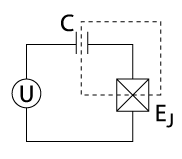
\includegraphics[width=0.3\linewidth]{md/Avance1/cooperpairbox.png}
\caption{Circuito de una caja de pares de Cooper}
\label{fig:cooperpairboxcircuit}
\end{figure}

\begin{figure}[H]
\centering 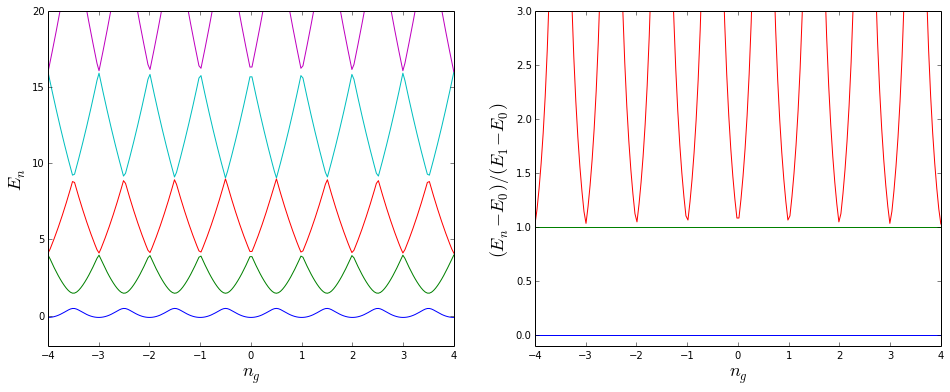
\includegraphics[width=0.3\linewidth]{md/Avance1/cooperenergy.png}
\caption{Niveles de energía de una caja de pares de Cooper}
\label{fig:cooperpairboxenergy}
\end{figure}

\end{frame}

\begin{frame}
    \frametitle{Transmon}

Intercambiamos anarmonicidad por independencia de $n_g$

\begin{figure}[H]
\centering 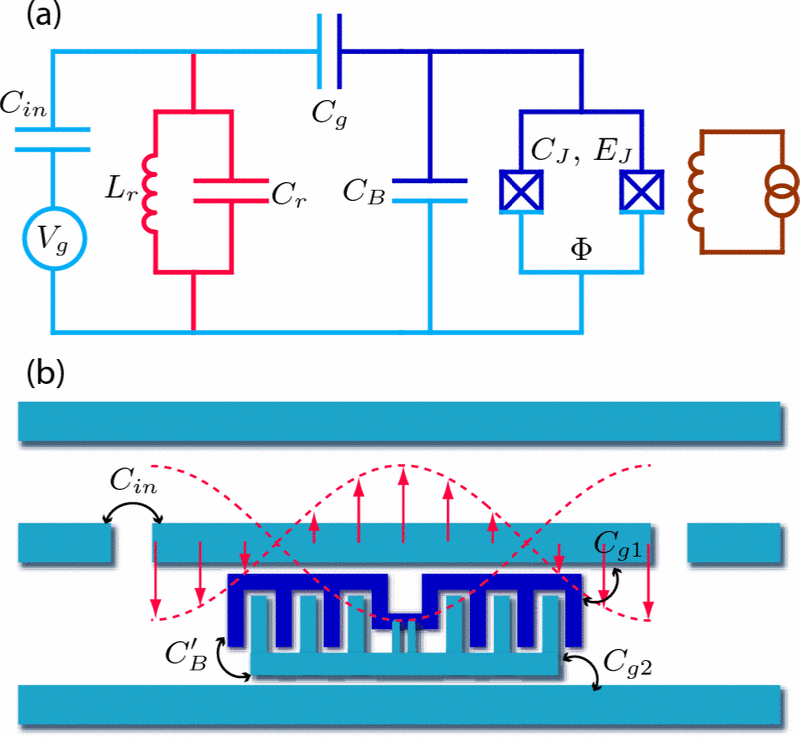
\includegraphics[width=0.3\linewidth]{md/Avance1/transmon.png}
\caption{Circuito de un transmon}
\label{fig:transmoncircuit}
\end{figure}

\begin{figure}[H]
\centering 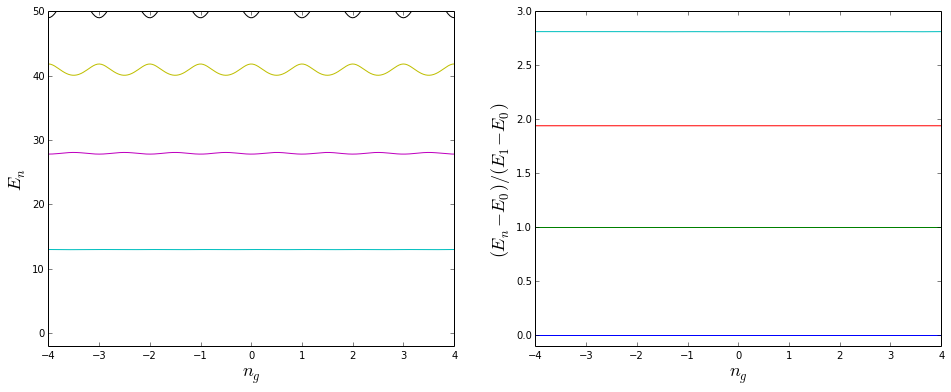
\includegraphics[width=0.3\linewidth]{md/Avance1/transmonenergy.png}
\caption{Niveles de energía de un transmon}
\label{fig:transmonenergy}
\end{figure}

\end{frame}

\begin{frame}
    \frametitle{Modelo de Jaynes-Cummings}

$$\hat{H} = \hat{H}_c + \hat{H}_q + \hat{H}_{qc} = \hbar \omega_c (a^\dag a + 
  \frac{1}{2}) + \frac{1}{2} \hbar \omega_q \sigma_z + \hbar g \sigma_x (a+a^\dag)$$

\justify
De ahora en adelante $\hbar = 1$ y despreciaré los términos constantes, pues 
sólo contribuyen en fases globales a la evolución del sistema.

\end{frame}

\begin{frame}
    \frametitle{Aproximación de onda rotacional}

$$\hat{H}_{qc} = \hat{H}_{qc}^{JC} + \hat{H}_{qc}^{AJC} = g(a \sigma_+ + 
  a^\dag\sigma_-) + g(a^\dag \sigma_+ + a \sigma_-)$$

$$\hat{H} = \hat{H}_c + \hat{H}_q + \hat{H}_{qc} = \omega_c a^\dag a +
  \frac{1}{2} \omega_q \sigma_z + g(a \sigma_+ + a^\dag \sigma_-)$$

  \end{frame}
  
  \begin{frame}
      \frametitle{Hamiltoniano multiquibit}

$$\hat{H} = \hat{H}_q + \hat{H}_{qc} = \frac{1}{2} \sum\limits_i \omega_{qi} 
  \sigma_{zi} + \sum\limits_i g_i (a \sigma_{+ i} + a^\dagger \sigma_{- i})$$

  \end{frame}
  
  \begin{frame}
      \frametitle{Pulsos de microondas}

$$\hat{H}_d = \sum\limits_k (a+a^\dagger) (\xi_k e^{-i\omega_d^{(k)}t} + 
  \xi_k^*e^{i\omega_d^{(k)}t})$$

RWA: $$\hat{H}_d=\sum\limits_k a\xi_k^*e^{i\omega_d^{(k)}t}+
  a^\dagger\xi_ke^{-i\omega_d^{(k)}t}$$

  \end{frame}
  
  \begin{frame}
      \frametitle{Régimen rotacional del pulso}

\justify
Trabajando con un sólo modo a la vez, se aplica la siguiente transformación $U(t) 
= exp[-i \omega_d t(a^\dagger a + \sum\limits_i \sigma_{z i})]$ para entrar en 
el régimen rotacional del pulso de control.

$$\hat{H} = U^\dagger (\hat{H}_{syst} + \hat{H}_d) U - i U^\dagger \dot{U}$$
$$ \hat{H} = \Delta_c a^\dagger a + \frac{1}{2} \sum\limits_i \Delta_{qi} 
  \sigma_{zi} + \sum\limits_i g_i (a \sigma_{+ i} + a^\dagger \sigma_{- i}) + 
  (a\xi^*e^{i\omega_d t}+a^\dagger\xi e^{-i\omega_d t})$$

$\Delta_c = \omega_c - \omega_d \qquad \quad \Delta_{qi} = \omega_{qi} - \omega_d$

\end{frame}

\begin{frame}
    \frametitle{Efecto del pulso sobre el qubit}

\justify
Luego se aplica el operador de desplazamineto $D(\alpha) = exp[\alpha a^\dagger - 
\alpha^* a]$ sobre el campo $a$ con $\dot{\alpha} = -i \Delta_c \alpha -i \xi 
e^{-i \omega_d t}$ para eliminar el efecto directo del pulso sobre la cavidad.

$$\hat{H} = D^\dagger (\alpha) \hat{H}_{old} D(\alpha) -i D^\dagger(\alpha) \dot{D}(\alpha)$$

$$\hat{H} = \Delta_c a^\dagger a + \frac{1}{2} \sum\limits_i \Delta_{qi} 
  \sigma_{zi} + \sum\limits_i g_i (a \sigma_{+i} + a^\dagger \sigma_{-i})$$
$$ + \sum\limits_i g_i (\alpha \sigma_{+i} + \alpha^* \sigma_{-i}) - \Delta_c
  \alpha \alpha^* $$

El término $-\Delta_c \alpha \alpha^*$ se desprecia, ya que sólo representa 
una fase global en la evolución del sistema.

\end{frame}

\begin{frame}
    \frametitle{Régimen dispersivo}

\justify
Finalmente, aplicamos la transformación $U = exp[\sum\limits_i \frac{g_i}
{\Delta_i} (a^\dagger \sigma_{-i} - a \sigma_{+i})]$, donde $\Delta_i = 
\omega_{qi} - \omega_c$ y realizamos la aproximación de segundo grado sobre
los términos $\frac{g_i}{\Delta_i} \ll 1$.

$$\hat{H} = U^\dagger \hat{H}_{old} U$$
$$\hat{H} \approx \tilde{\Delta}_c a^\dagger a + \frac{1}{2} \sum\limits_i
  \tilde{\Delta}_{qi} \sigma_{zi} + \sum\limits_i (\Omega_i \sigma_{+i} +
  \Omega_i^* \sigma_{-i})$$
$$+ \sum\limits_{i \neq j} \frac{g_i g_j}{2 \Delta_i} 
  (\sigma_{-i} \sigma_{+j}+\sigma_{+i} \sigma_{-j})$$

$\tilde{\Delta}_c = (\omega_c + \sum\limits_i \chi_i \sigma_{zi}) - \omega_d
 \qquad
 \tilde{\Delta}_{qi} = (\omega_{qi} + \chi_i) - \omega_d
 \qquad
 \chi_i = \frac{g_i^2}{\Delta_i}$

 \end{frame}
 
 \begin{frame}
     \frametitle{Rotaciones X-Y}

\justify
Tomando $\Omega(t) = \Omega^x(t) \cos(\omega_d t) + \Omega^y \sin(\omega_d t)$,
donde $\omega_d$ es igual a la frecuencia de resonancia de uno de los qubits
logramos rotaciones sobre los ejes X e Y. Las amplitudes de estas rotaciones
vienen dadas por $\int_0^{t_0} \Omega^x(t) dt$ y $\int_0^{t_0} \Omega^y(t)
dt$, respectivamente, donde $t_0$ es la duración del pulso.

$$\hat{H} \approx \tilde{\Delta}_c a^\dagger a + \frac{1}{2} \tilde{\Delta}_q 
  \sigma_z + \frac{1}{2} (\Omega^x(t) \sigma_x + \Omega^y(t) \sigma_y)$$

  \end{frame}
  
\begin{frame}
  \frametitle{Compuerta de entrelazamiento}

Ejemplo con sólo dos qubits

$$\hat{H} \approx \frac{1}{2} \tilde{\Delta}_{q_1} \sigma_{z_1} + 
  \frac{1}{2} \tilde{\Delta}_{q_2} \sigma_{z_2} + 
  \frac{g_1 g_2 (\Delta_1 + \Delta_2)}{2 \Delta_1 \Delta_2} 
  (\sigma_{-_1} \sigma_{+_2} + \sigma_{+_1} \sigma_{-_2})$$

Variando la frecuencia de resonacia de los qubit, se puede variar el 
acoplamiento entre estos. 

\end{frame}

\section{Simulador}

\begin{frame}
    \frametitle{Parámetros de los sistemas simulados}

    \begin{enumerate}
        \item Frecuencias de resonancia:
            \begin{enumerate}
                \item Resonador: 10GHz
                \item Qubit 0: 5GHz
                \item Qubit 1: 6GHz
                \item Qubit 2: 7GHz
                \item Qubit 3: 8GHz
                \item *Qubit 4: 11GHz
                \item *Qubit 5: 12GHz
                \item *Qubit 6: 13GHz
                \item *Qubit 7: 14GHz
            \end{enumerate}
        \item Constante de acoplamiento: Todas iguales a 0.1GHz
        \item Tasas de relajación: Todas iguales a 25KHz
        \item Tiempo de relajación: Todos iguales a $40 \mu s$
        \item Frecuencia de resonancia para iSWAP: 9GHz
    \end{enumerate}

    *Sólo aplica para el caso del sistema de 8 qubits

\end{frame}

\begin{frame}
    \frametitle{Compuertas compuestas}

\end{frame}

\section{Algoritmo de Grover}

\begin{frame}
    \frametitle{Operadores de reflexión}

    \begin{align}
        \Pi_\mathcal{W} &= \sum_k \ketbra{\omega_k} \\
        \ket{\psi} &= \sin(\theta) \ket{\psi_1} + \cos(\theta) \ket{\psi_0}
    \end{align}

    \begin{align}
        U_\mathcal{W} &= 2 \mathds{1} - 2 \Pi_\mathcal{W}\\
        U_\psi &= 2 \ketbra{\psi} - \mathds{1}
    \end{align}
\end{frame}

\begin{frame}
    \frametitle{Algoritmo de Grover}

\begin{figure}[H]
\[ \Qcircuit @C=1.4em @R=1.8em {
\lstick{\ket{0}} & {/^n} \qw & \gate{H^{\otimes n}} & \gate{U_{\omega}} & \gate{U_s} & \meter & \cw \\
& & & \rstick{\hspace{-13pt} k_{max} \text{ veces}}
\gategroup{1}{4}{1}{5}{1.5em}{_\}}
} \]
\caption{Circuito del algoritmo de Grover, $k_{max}$ desconocido.}
\end{figure}

\begin{figure}[H]
\centering 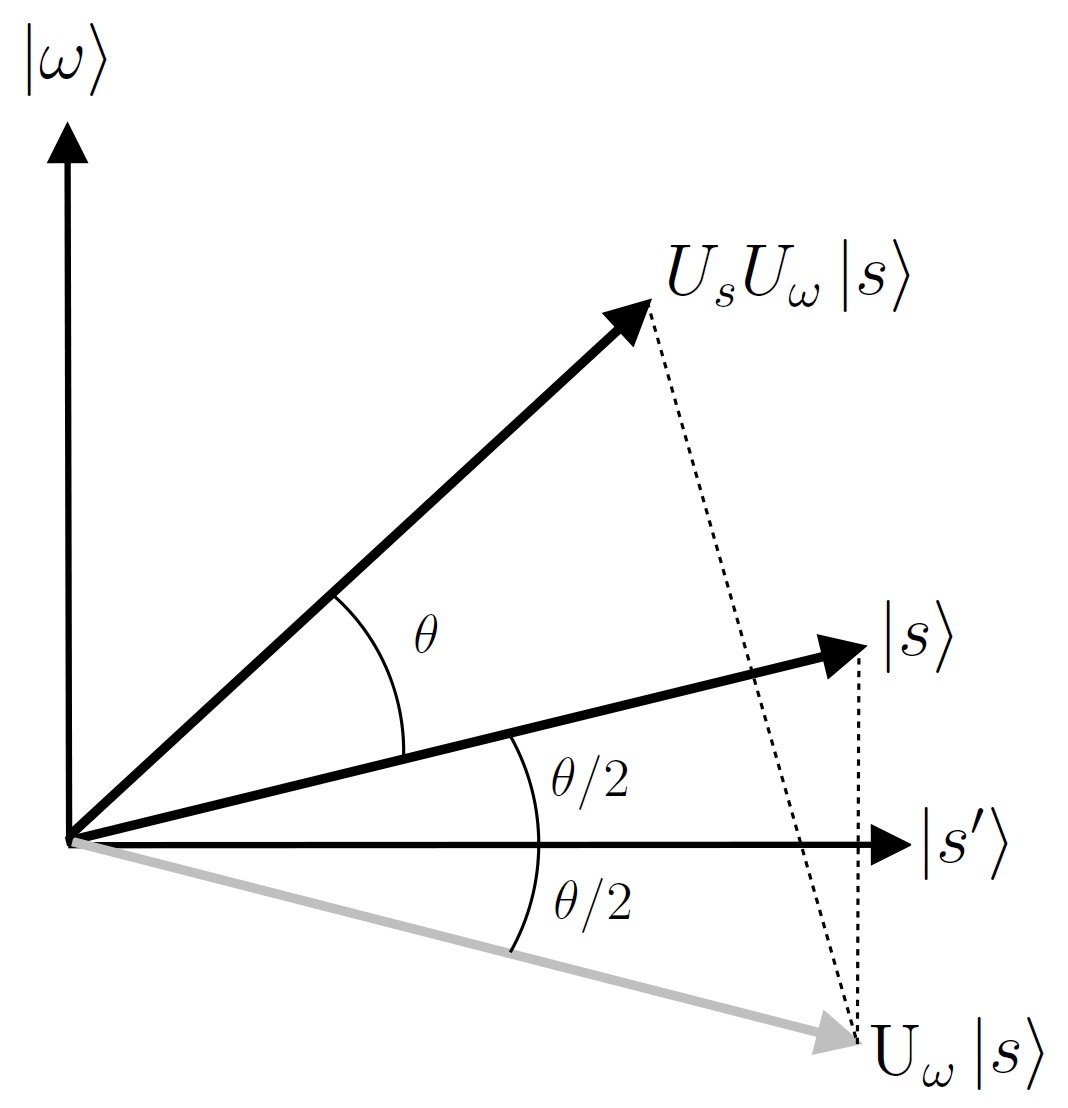
\includegraphics[width=0.3\linewidth]{img/grover_geometry.png}
\caption{Interpretación geométrica del operador difusión}
\label{fig:groverdifusion}
\end{figure}


El circuito cuántico asociado al algoritmo de Grover tiene la siguiente representación:

\begin{figure}[H]
\[ \Qcircuit @C=1.4em @R=1.8em {
\lstick{\ket{0}} & {/^n} \qw & \gate{H^{\otimes n}} & \gate{U_{\omega}} & \gate{U_s} & \meter & \cw \\
& & & \rstick{\hspace{-13pt} \lfloor\frac{\pi \sqrt{N}}{4}\rfloor \text{ veces}}
\gategroup{1}{4}{1}{5}{1.3em}{_\}}
} \]
\caption{Circuito del algoritmo de Grover.}
\end{figure}

Dicho algoritmo se puede describir detalladamente en los siguientes pasos:

\begin{enumerate}
    \item Preparar el estado fiducial.
    \item Aplicar la transformada de Walsh-Hadamard.
    \item Realizar la iteración de Grover $\lfloor \frac{\pi}{4} \sqrt{N} \rfloor$ veces.
    \begin{enumerate}
        \item Aplicar $U_{\omega}$.
        \item Aplicar $U_s$.
    \end{enumerate}
    \item Realizar la medida $\Omega$.
\end{enumerate}

\end{frame}

\begin{frame}
    \frametitle{Variaciones del algoritmo de Grover}

    \begin{enumerate}
        \item Algoritmo de amplificación de amplitud:
            Esta es una generalización del algoritmo de Grover, que permite utilizar un estado inicial genérico $\ket{\psi}$ y bases de datos con más de un estado deseado $\ket{\omega}$.
        \item Algoritmo de Grover en un paso:
            En lugar de realizar repetidas iteraciones del algoritmo, se realiza una sóla iteración, pero se ejecuta el algoritmo en varios sistemas simultáneamente.
        \item Optimización del algoritmo de Grover:
            Se ejecuta el algoritmo en varios sistemas simultáneamente, pero se realizan varias iteraciones.
    \end{enumerate}

\end{frame}

\begin{frame}
    \frametitle{Simulaciones del algoritmo de Grover}

\begin{figure}[H]
    \centering
    \begin{subfigure}[m]{0.49\textwidth}
        \centering
        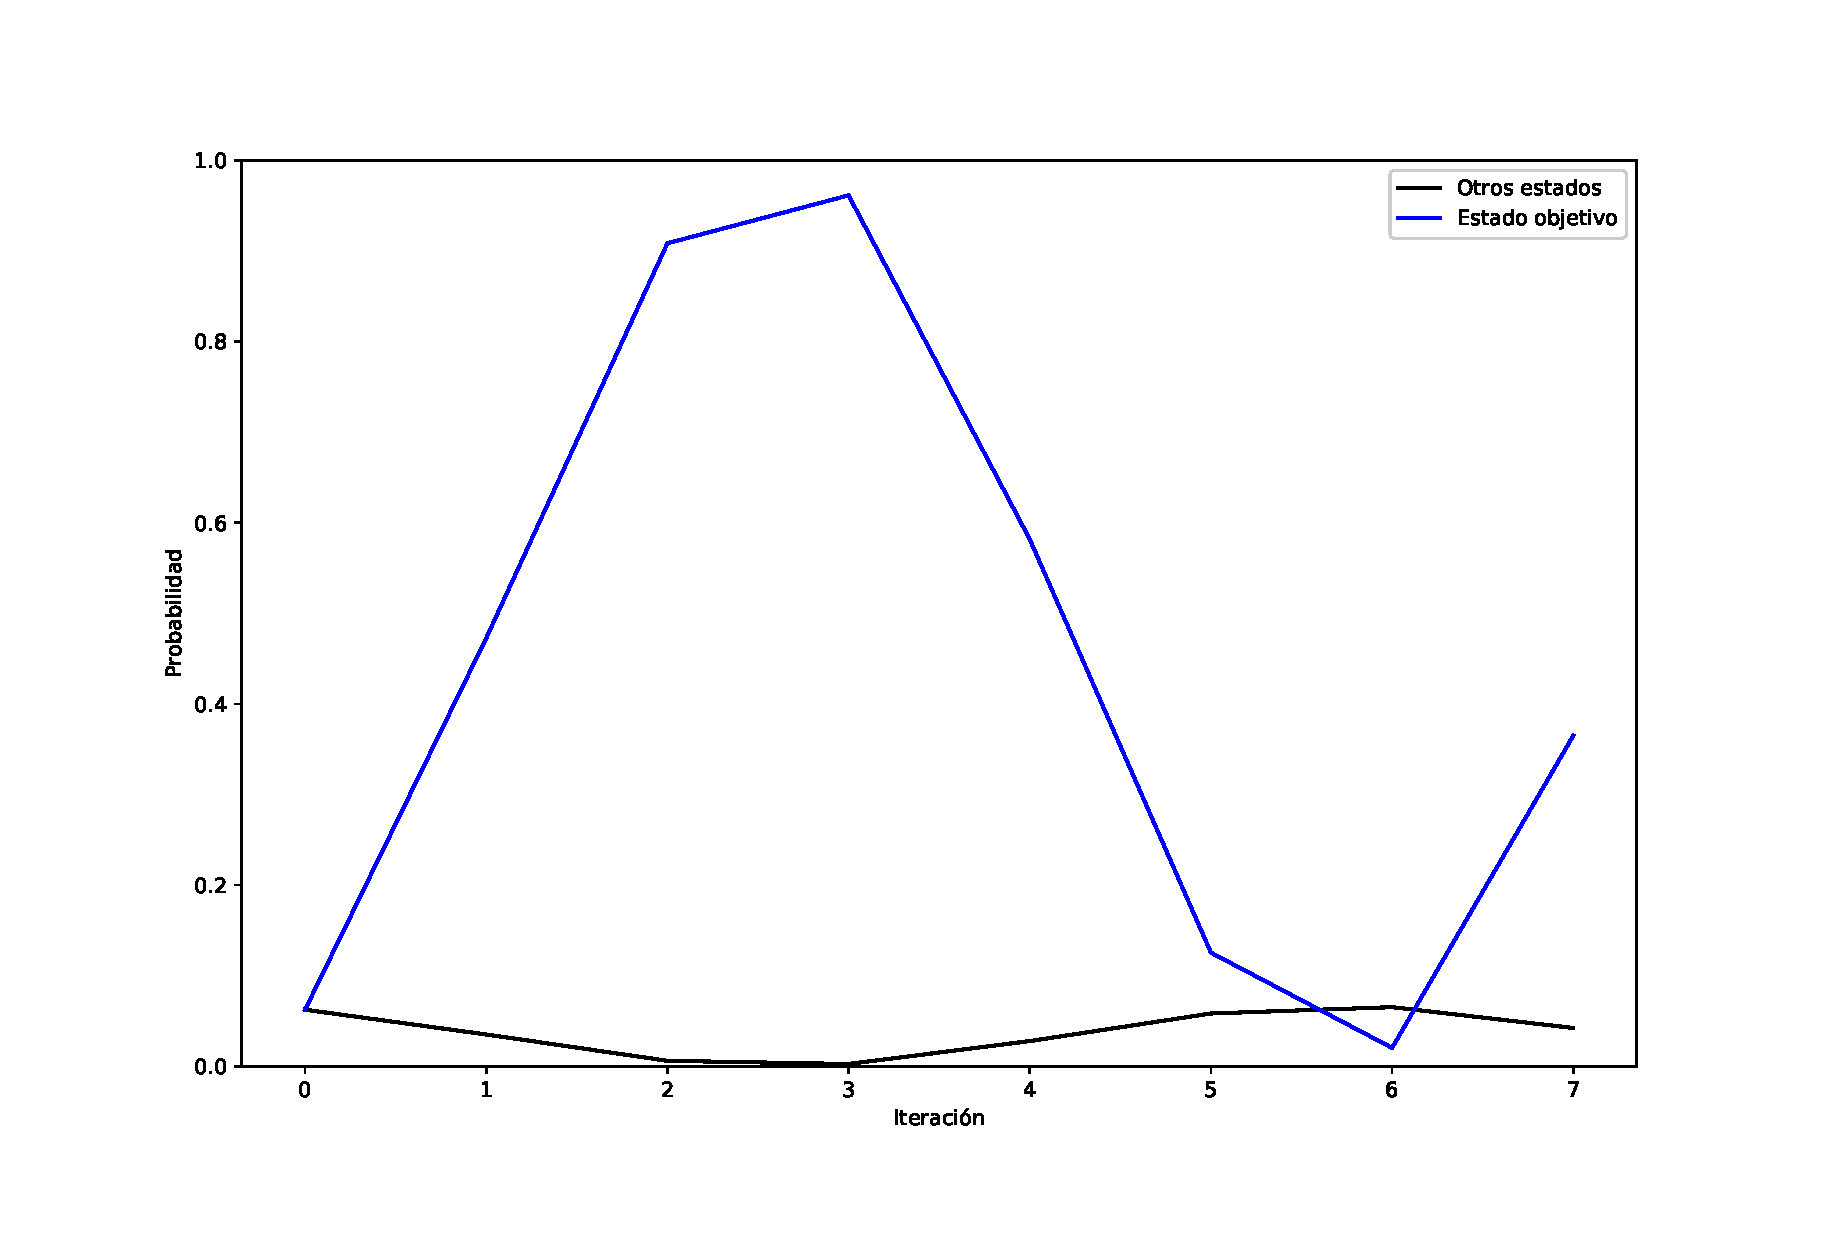
\includegraphics[width=0.9\linewidth]{img/groverallM.eps}
        \caption{Wolfram Mathematica}
    \end{subfigure}
    \begin{subfigure}[m]{0.49\textwidth}
        \centering
        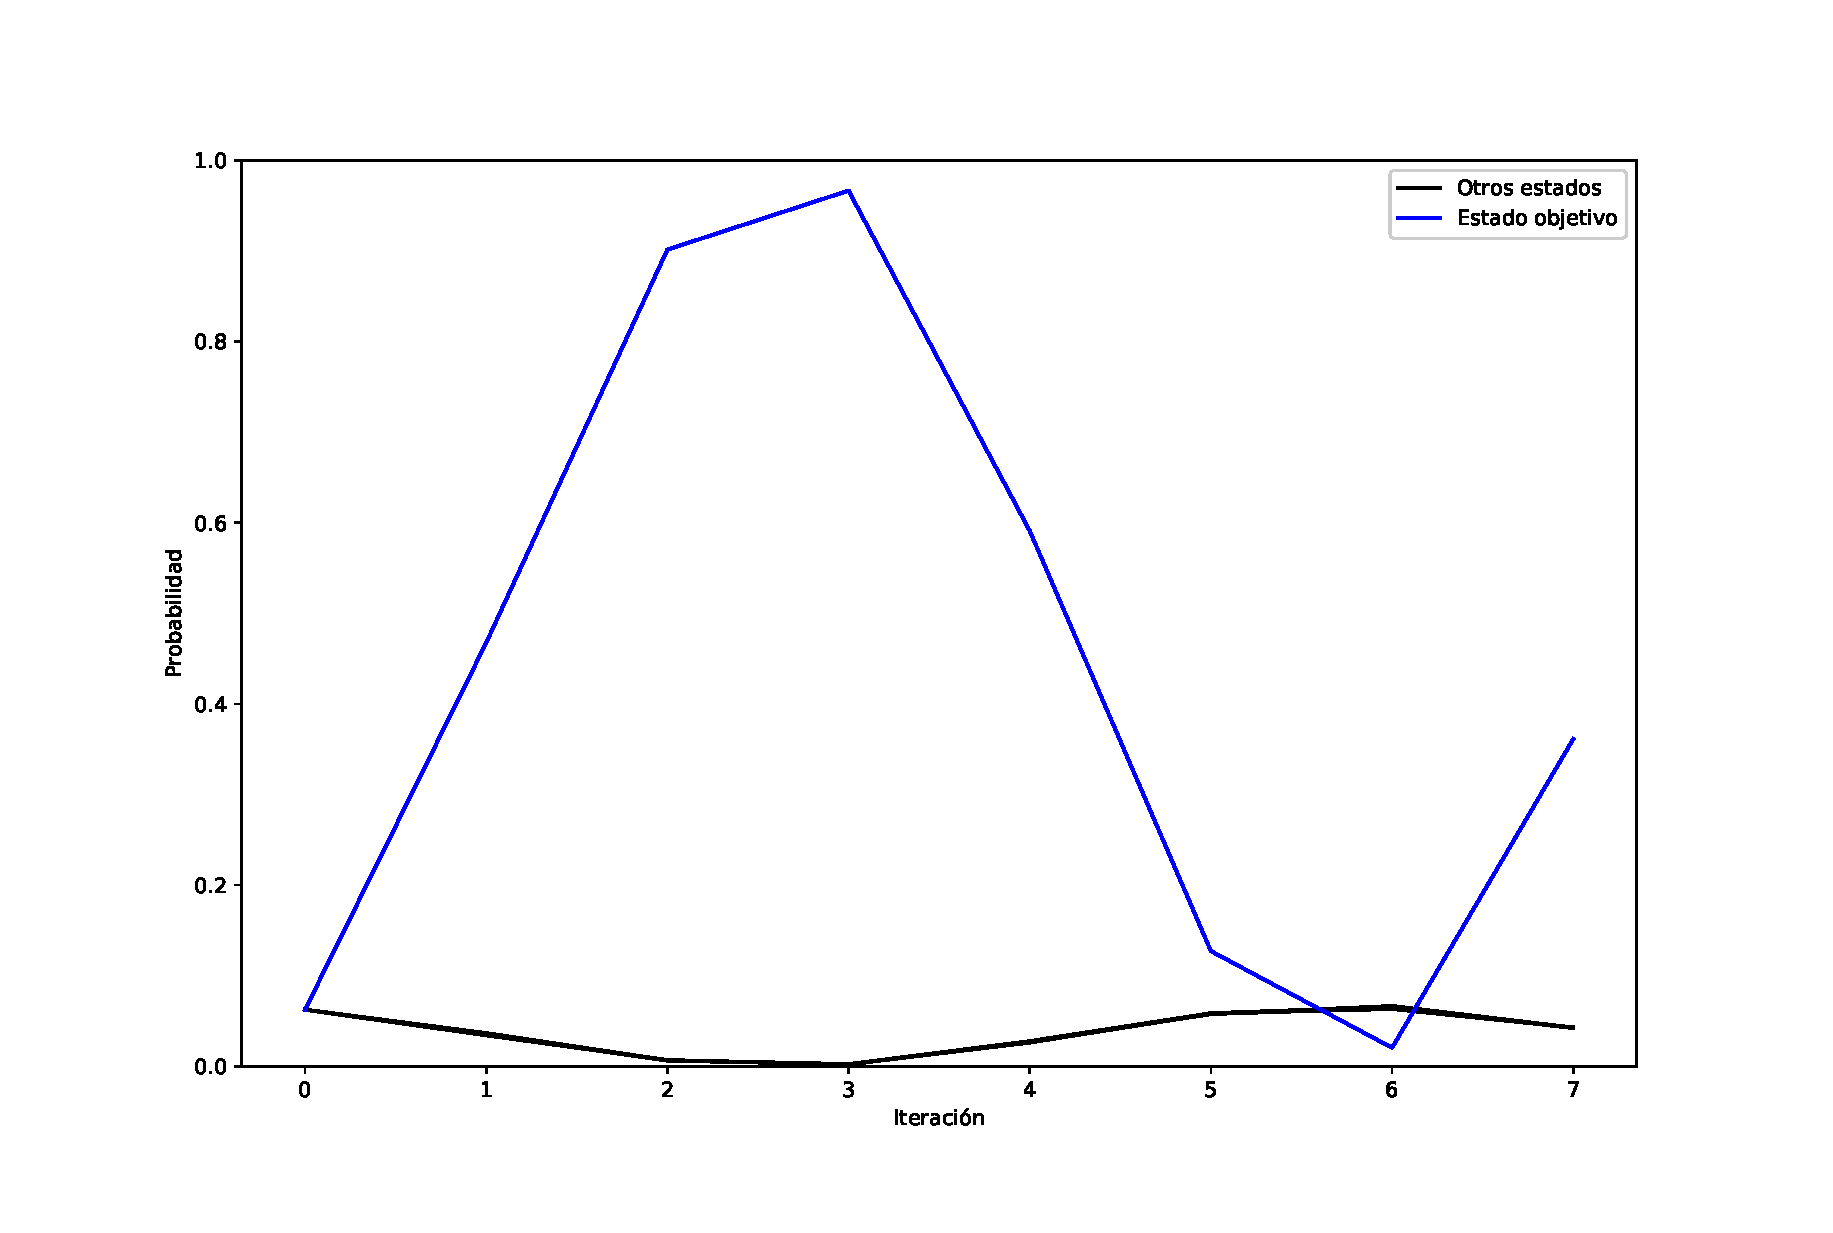
\includegraphics[width=0.9\linewidth]{img/groveralllossless.eps}
        \caption{Python}
    \end{subfigure}
    \caption[Evolución de las probabilidades en el algoritmo de Grover sin relajación]{Evolución de las probabilidades en el algoritmo de Grover sin relajación}
    \label{fig:groverlosslesscomp1111}
\end{figure}


\begin{figure}[H]
    \centering
    \begin{subfigure}[m]{0.49\textwidth}
        \centering
        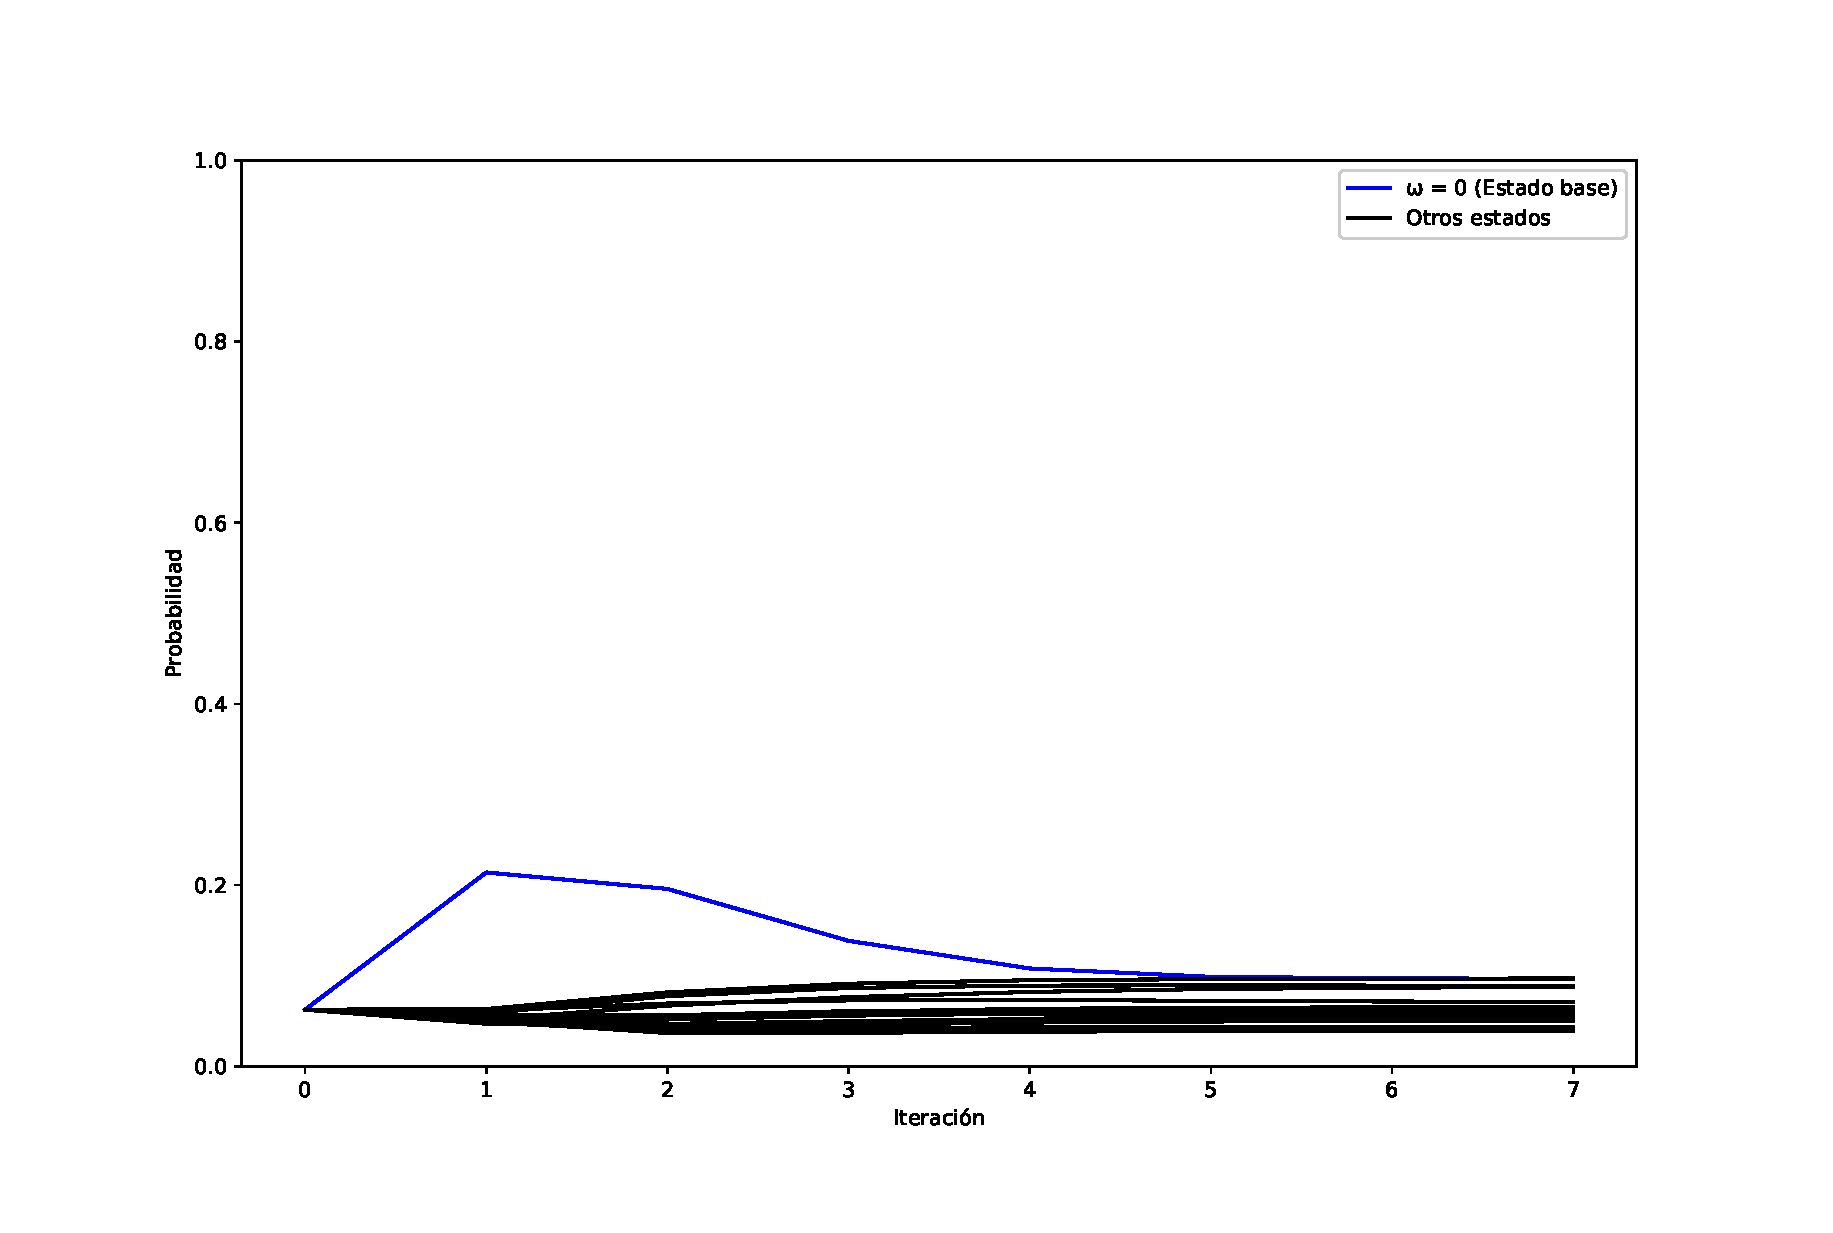
\includegraphics[width=0.99\linewidth]{img/grover0000loss.eps}
        \caption{$\omega = 0$}
        \label{fig:groverloss0000}
    \end{subfigure}
    \begin{subfigure}[m]{0.49\textwidth}
        \centering
        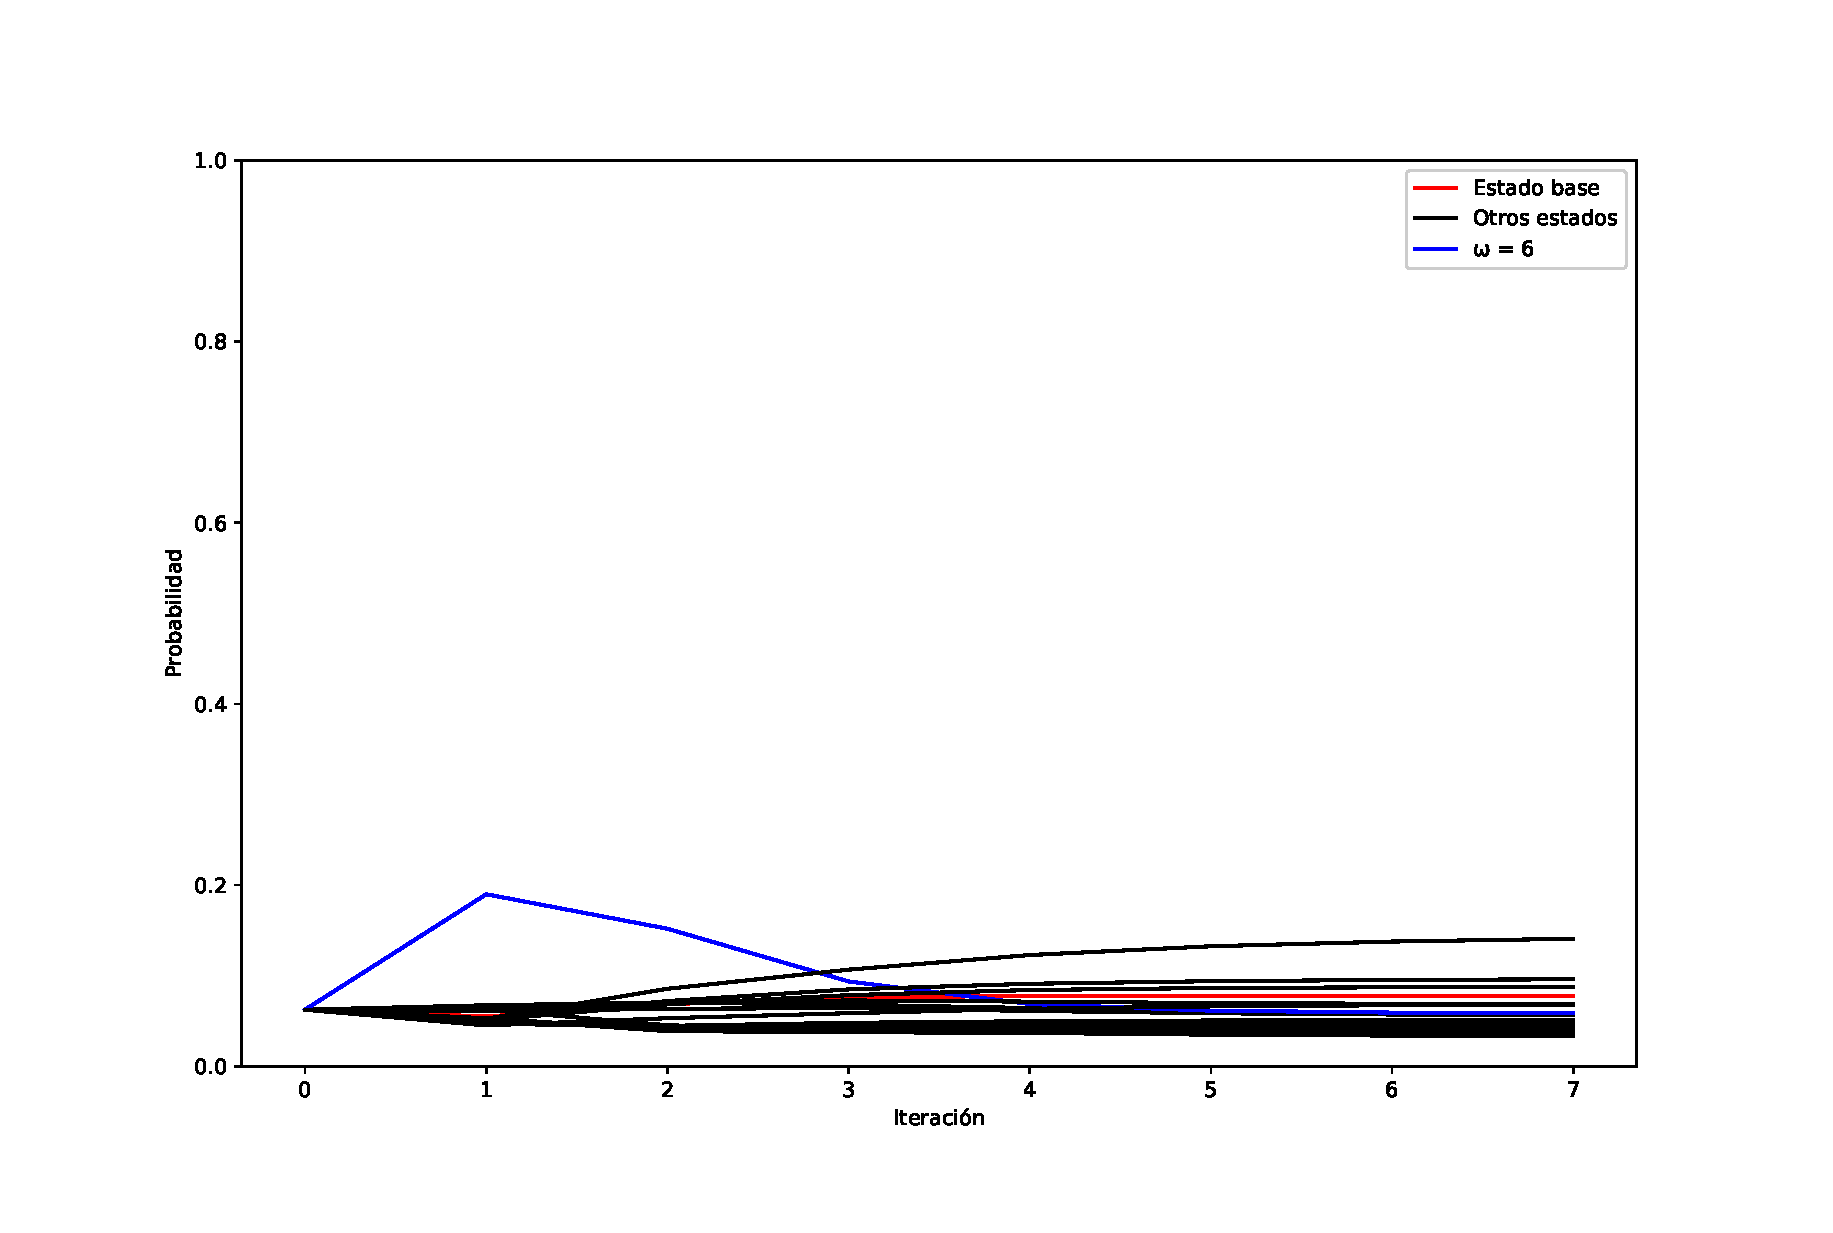
\includegraphics[width=0.99\linewidth]{img/grover0110loss.eps}
        \caption{$\omega = 6$}
        \label{fig:groverloss0110}
    \end{subfigure}
    \begin{subfigure}[m]{0.49\textwidth}
        \centering
        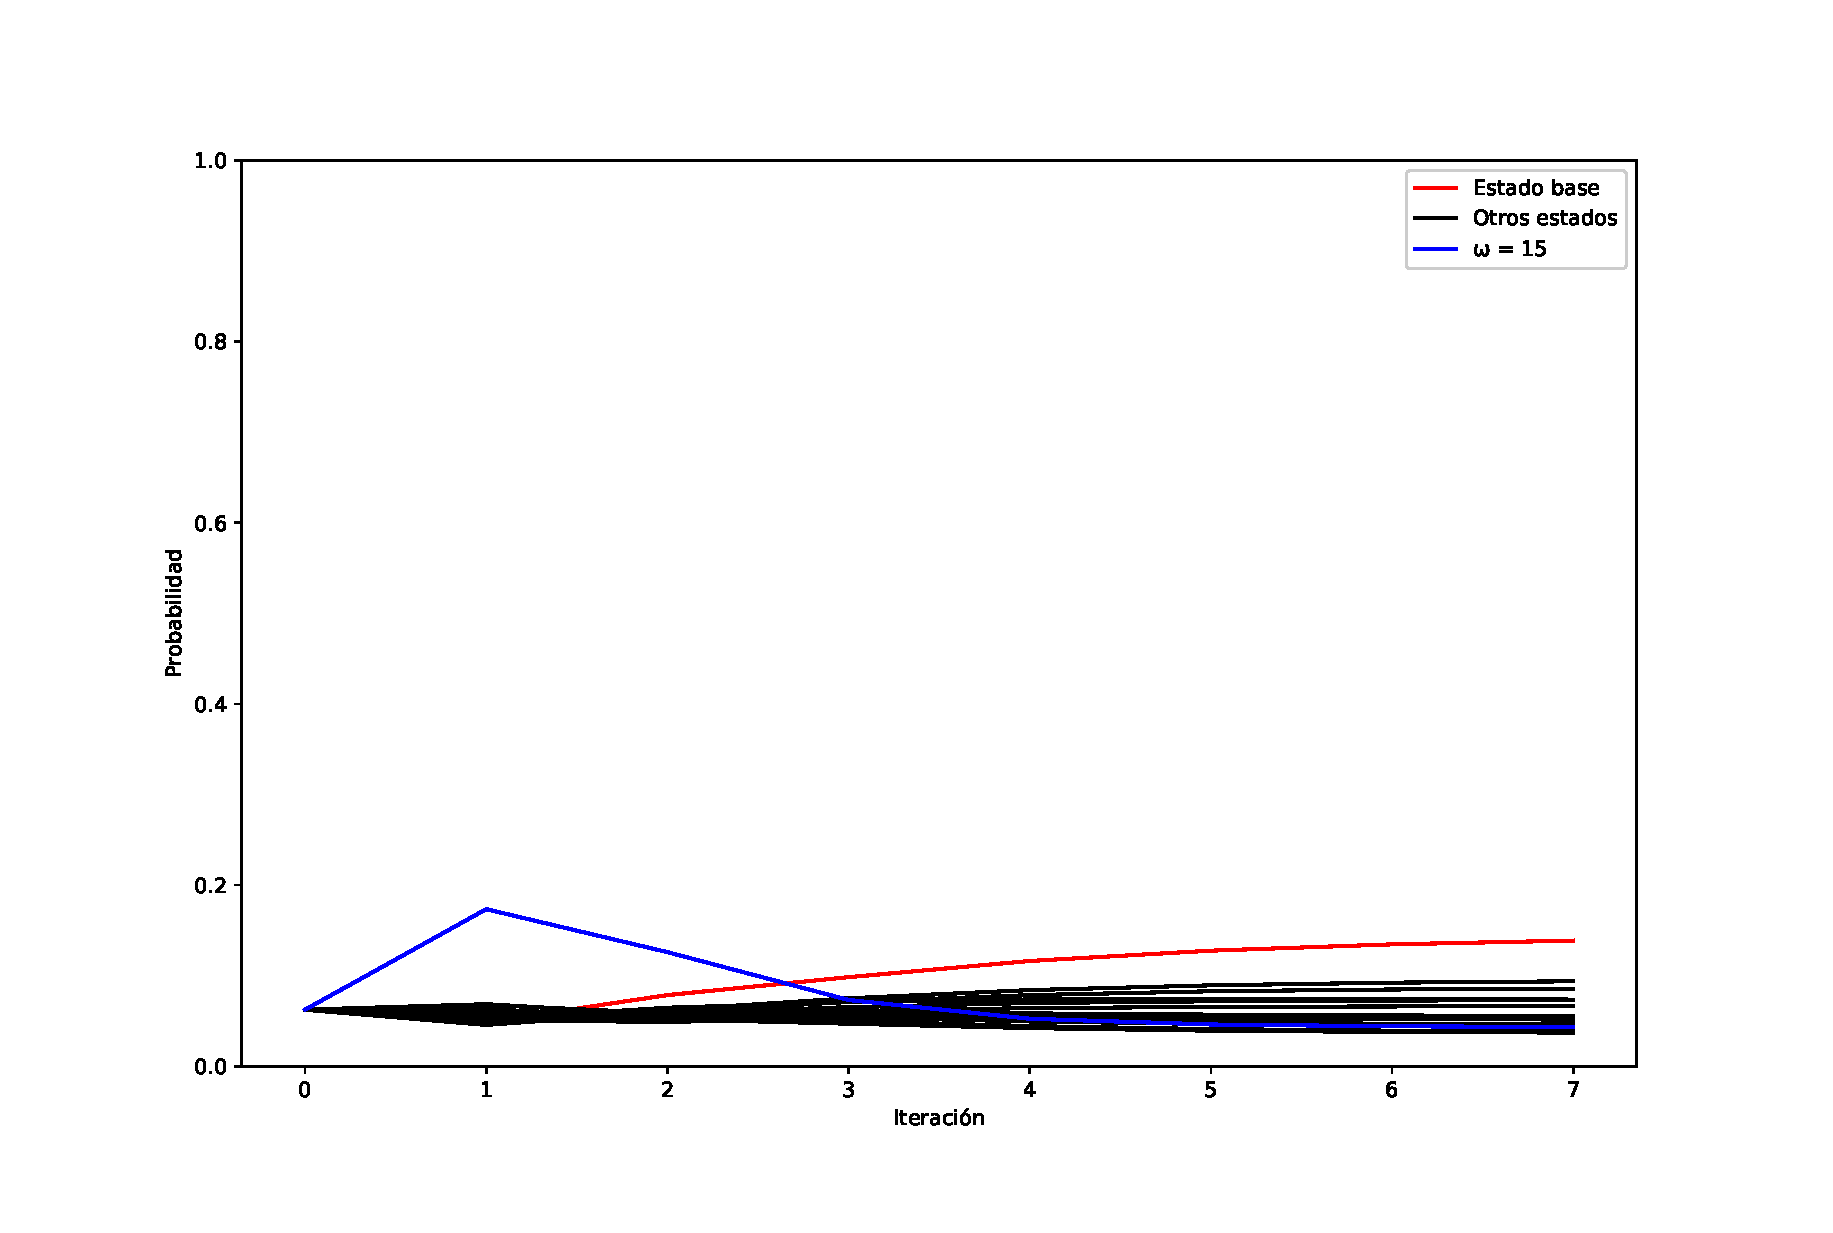
\includegraphics[width=0.99\linewidth]{img/groverallloss.eps}
        \caption{$\omega = 15$}
        \label{fig:groverloss1111}
    \end{subfigure}
    \caption[Evolución de las probabilidades en el algoritmo de Grover con relajación, $\mathcal{W} = \{0\}$]{Evolución de las probabilidades en el algoritmo de Grover con relajación. En (a) se tiene $\mathcal{W} = \{0\} = \{0000_2\}$, este es el caso que se ve menos afectado por el decaimiento de los qubits. En (b) se tiene $\mathcal{W} = \{6\} = \{0110_2\}$. En (c) se tiene $\mathcal{W} = \{15\} = \{1111_2\}$, este es el caso que se ve más afectado por el decaimiento de los qubits.}
    \label{fig:groverloss}
\end{figure}

\begin{figure}[H]
    \centering
    \begin{subfigure}[m]{0.49\textwidth}
        \centering
        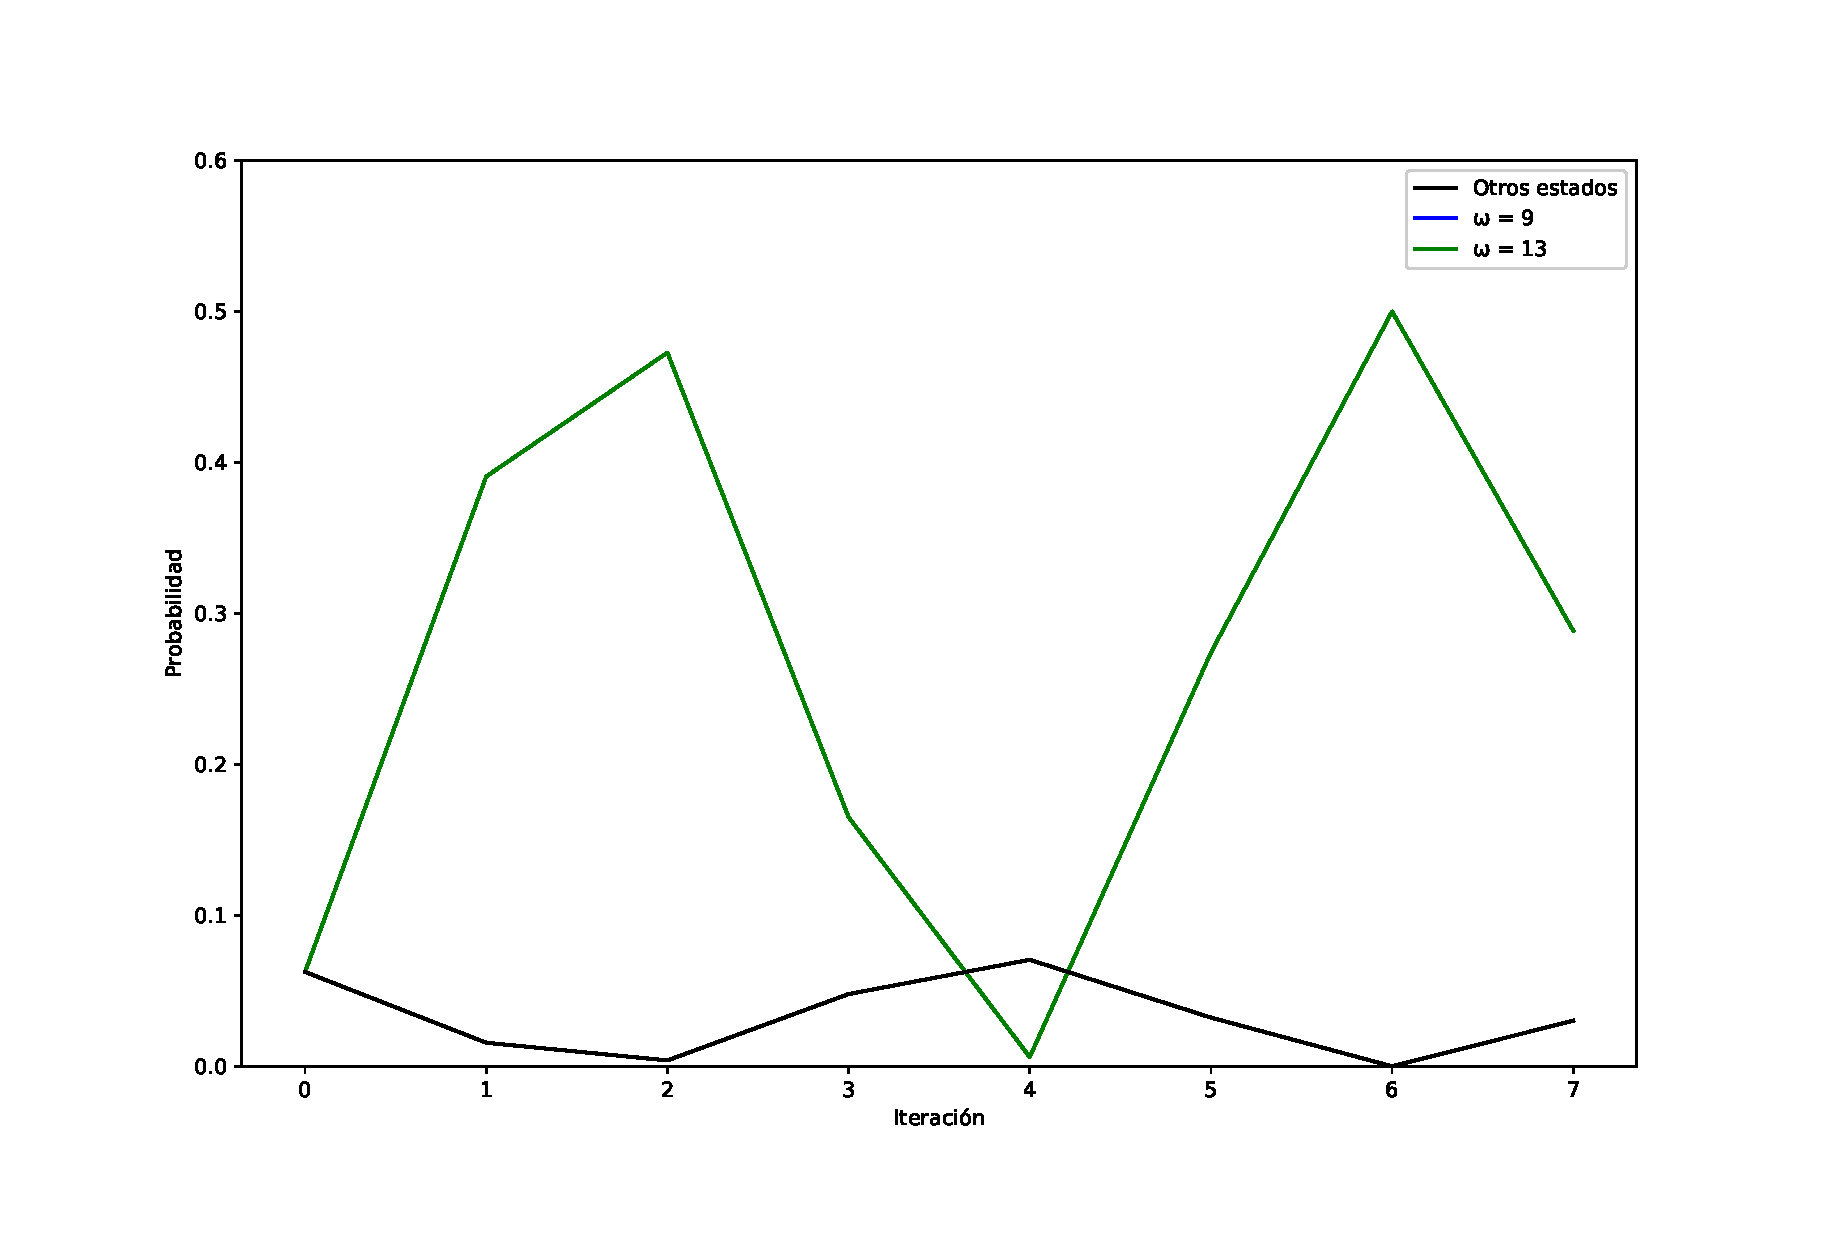
\includegraphics[width=0.9\linewidth]{img/grover2M.eps}
        \caption{Wolfram Mathematica}
    \end{subfigure}
    \begin{subfigure}[m]{0.49\textwidth}
        \centering
        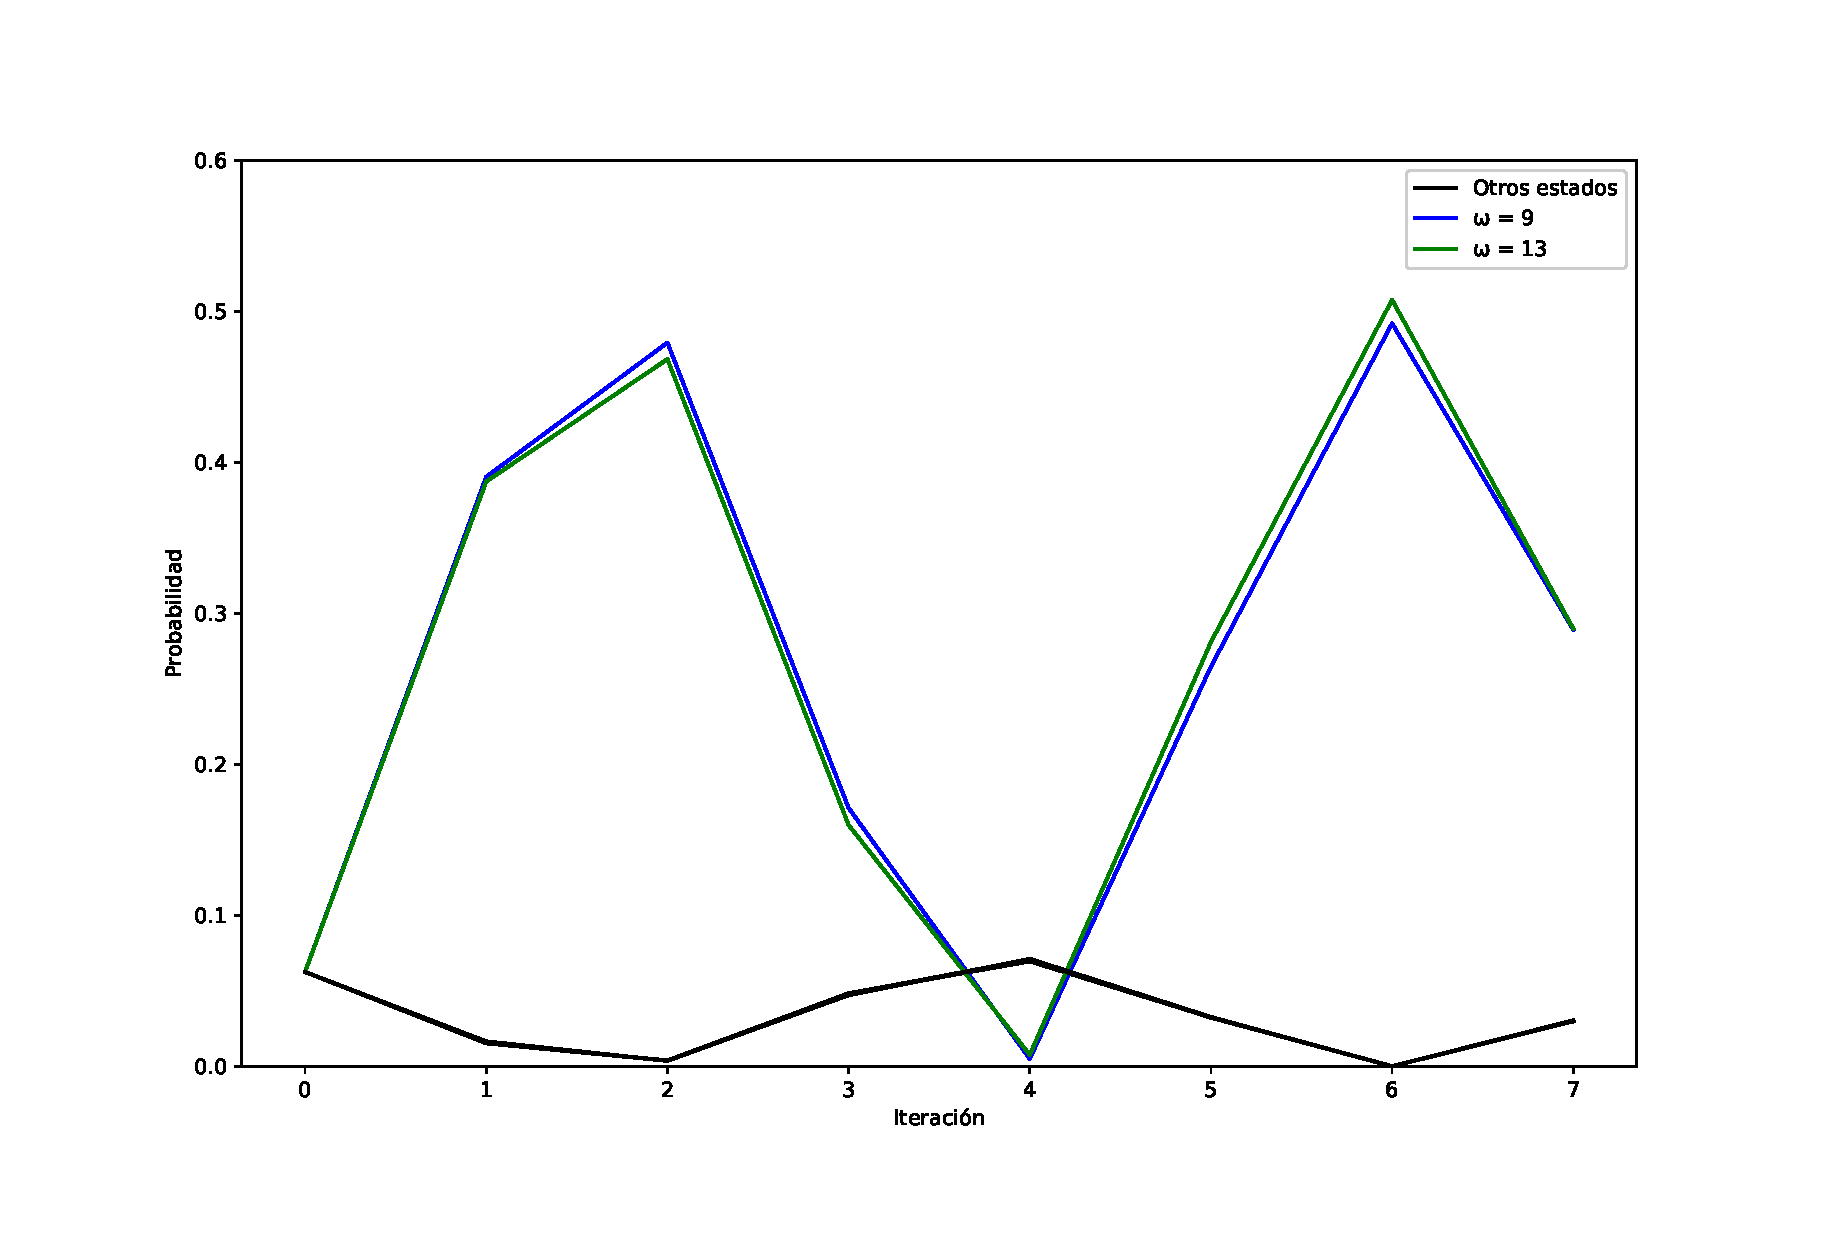
\includegraphics[width=0.9\linewidth]{img/grover2lossless.eps}
        \caption{Python}
    \end{subfigure}
    \caption[Evolución de las probabilidades en el algoritmo de amplificación de amplitud sin relajación, $\mathcal{W} = \{9, 13\}$]{Evolución de las probabilidades en el algoritmo de amplificación de amplitud sin relajación, $\mathcal{W} = \{9, 13\} = \{1001_2, 1101_2\}$}
    \label{fig:groverlosslesscomp2}
\end{figure}

\begin{figure}[H]
    \centering
    \begin{subfigure}[m]{0.49\textwidth}
        \centering
        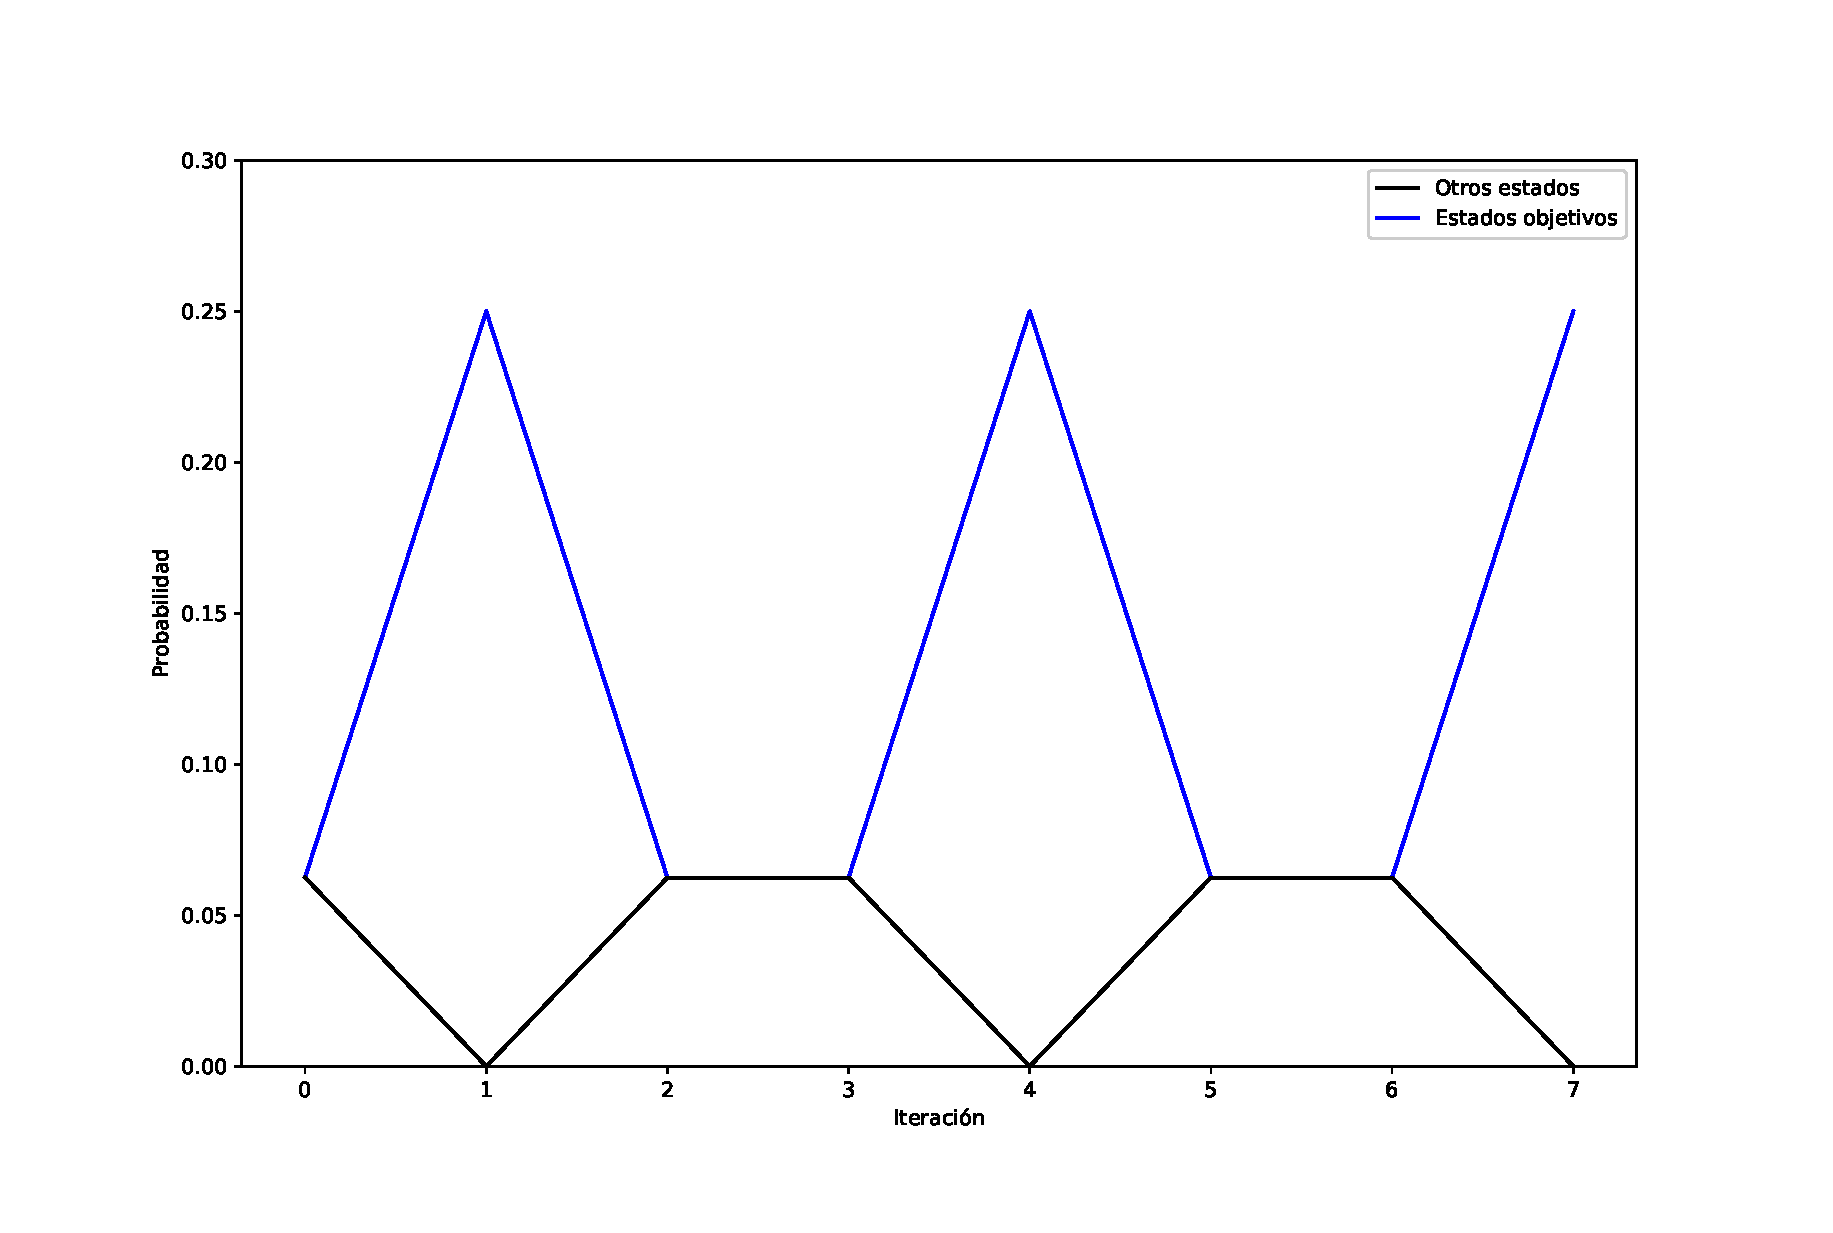
\includegraphics[width=0.9\linewidth]{img/grover3M.eps}
        \caption{Wolfram Mathematica}
    \end{subfigure}
    \begin{subfigure}[m]{0.49\textwidth}
        \centering
        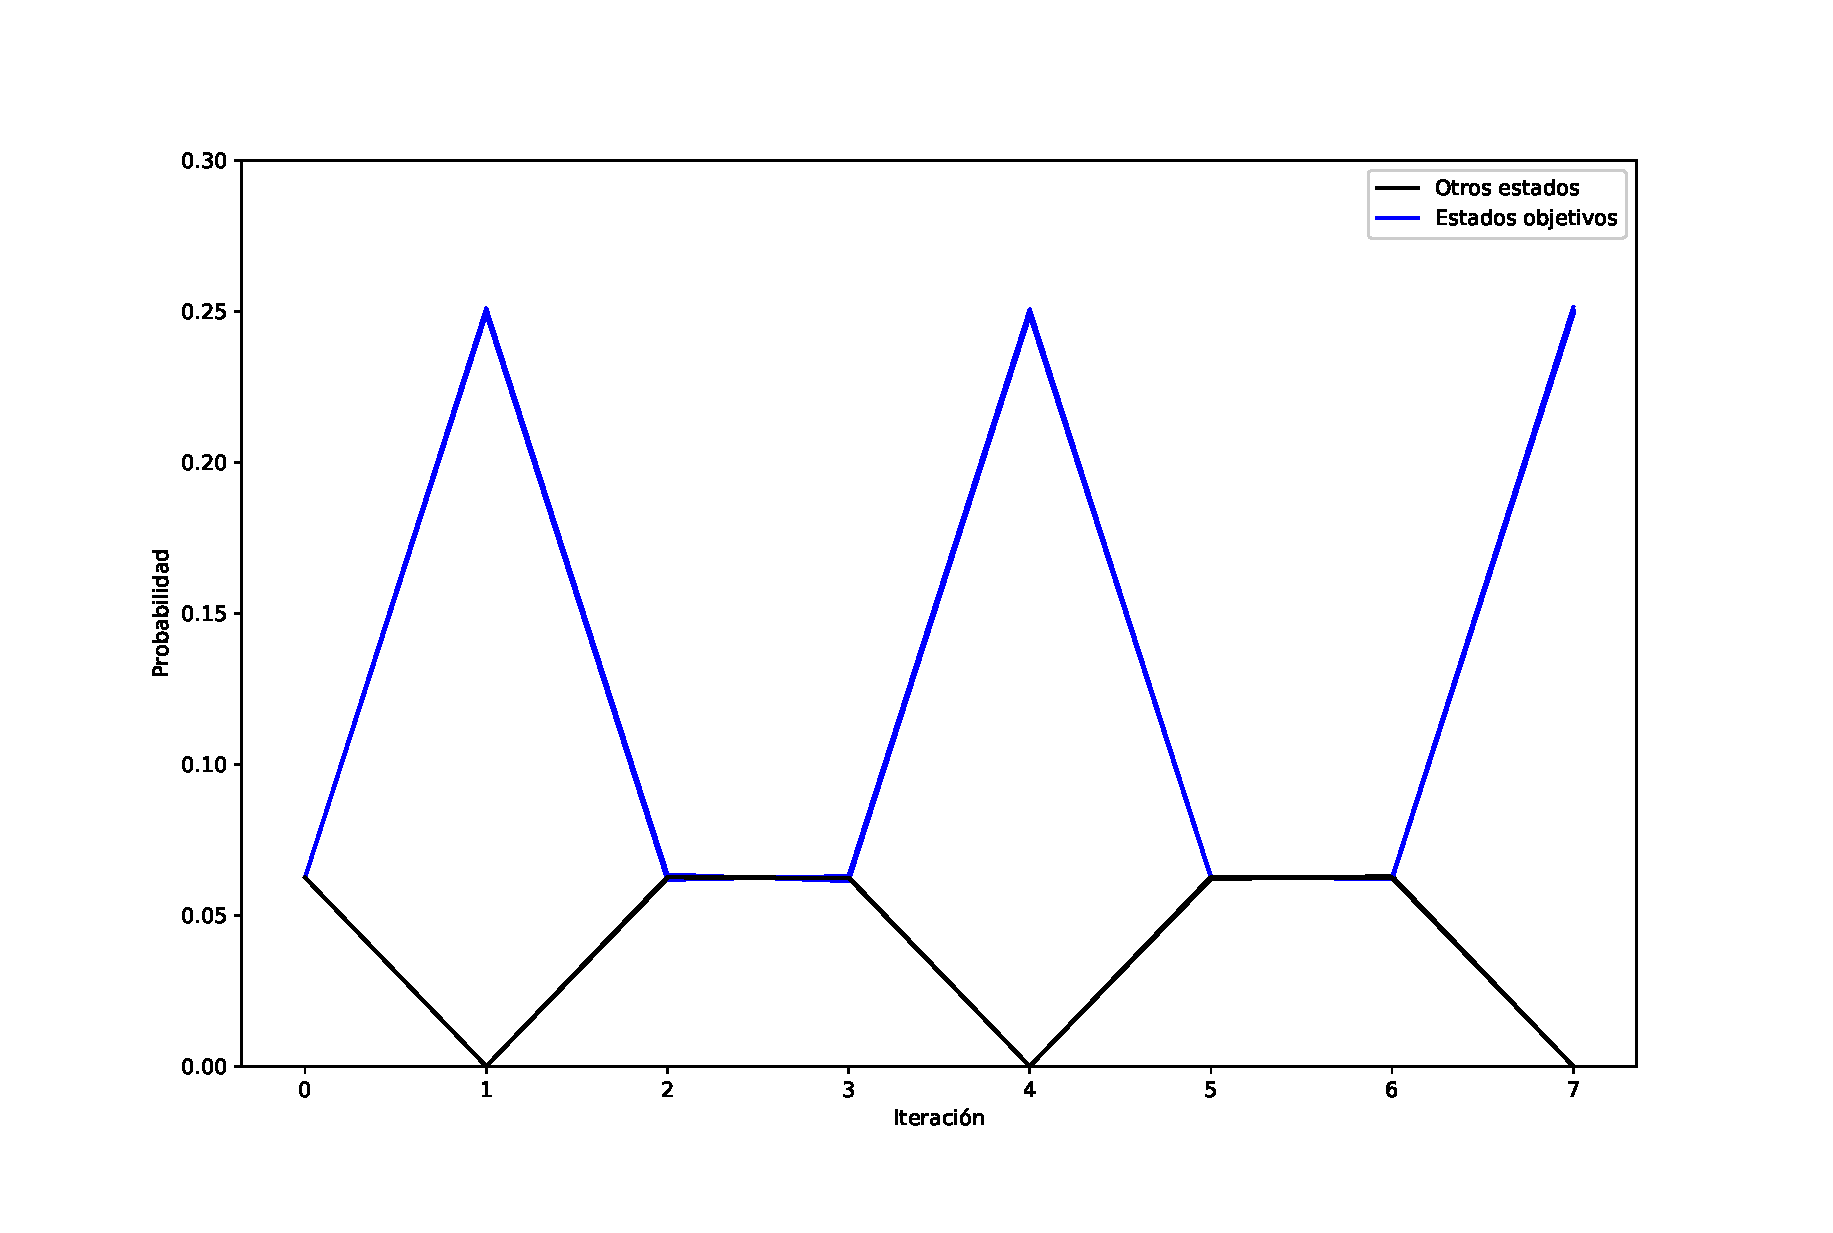
\includegraphics[width=0.9\linewidth]{img/grover3lossless.eps}
        \caption{Python}
    \end{subfigure}
    \caption[Evolución de las probabilidades en el algoritmo de amplificación de amplitud sin relajación, $\mathcal{W} = \{4, 5, 12, 13\}$]{Evolución de las probabilidades en el algoritmo de amplificación de amplitud sin relajación, $\mathcal{W} = \{4, 5, 12, 13\} = \{0100_2, 0101_2, 1100_2, 1101_2\}$}
    \label{fig:groverlosslesscomp3}
\end{figure}

\begin{figure}[H]
    \centering
    \begin{subfigure}[m]{0.49\textwidth}
        \centering
        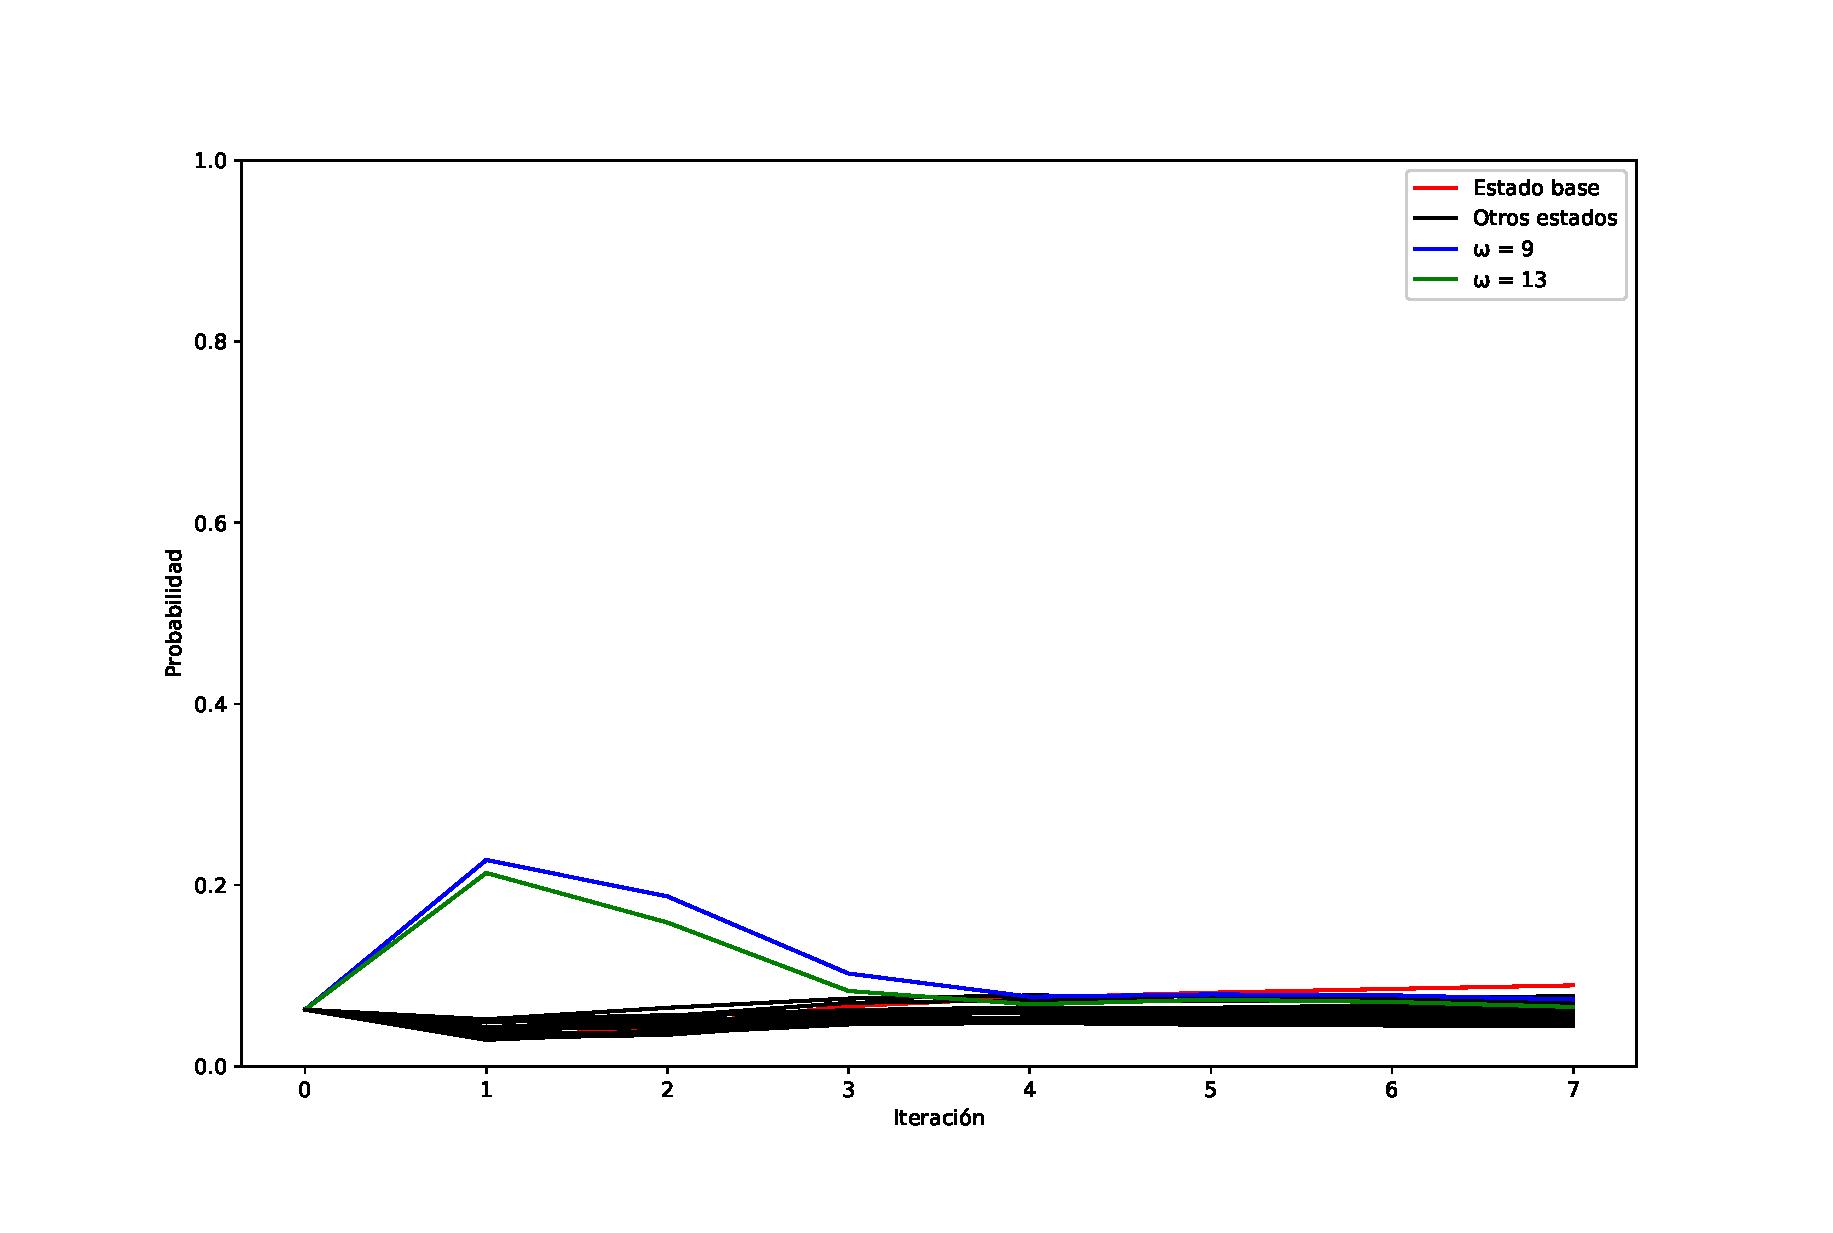
\includegraphics[width=0.99\linewidth]{img/grover2loss.eps}
        \caption{$\mathcal{W} = \{9, 13\}$}
    \end{subfigure}
    \begin{subfigure}[m]{0.49\textwidth}
        \centering
        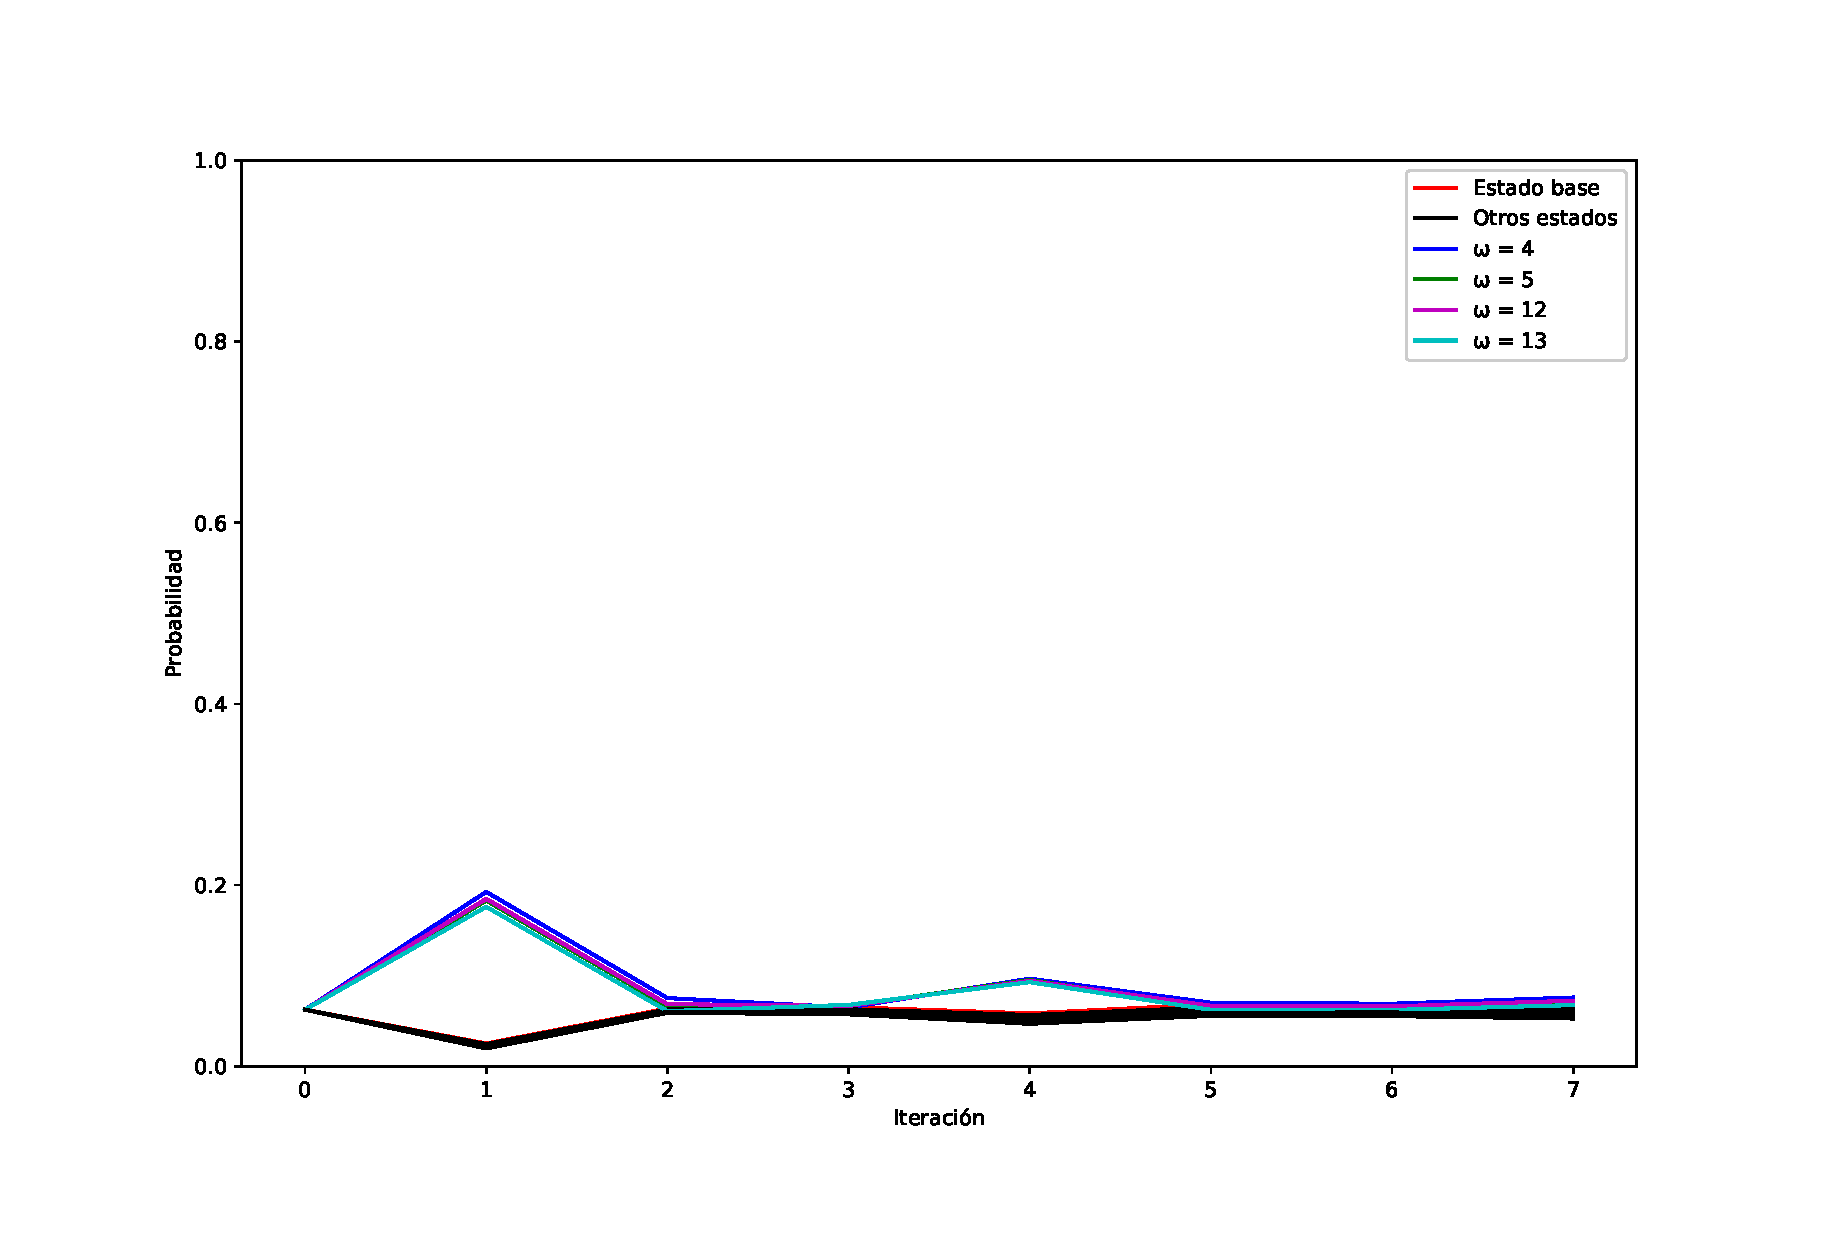
\includegraphics[width=0.99\linewidth]{img/grover3loss.eps}
        \caption{$\mathcal{W} = \{4, 5, 12, 13\}$}
    \end{subfigure}
    \caption[Evolución de las probabilidades en el algoritmo de amplificación de amplitud con relajación]{Evolución de las probabilidades en el algoritmo de amplificación de amplitud con relajación. En (a) se tiene $\mathcal{W} = \{9, 13\} = \{1001_2, 1101_2\}$, en (b) se tiene $\mathcal{W} = \{4, 5, 12, 13\} = \{0100_2, 0101_2, 1100_2, 1101_2\}$}
    \label{fig:groverlosscomp2}
\end{figure}

\end{frame}

\section{Algoritmo de Shor}

\begin{frame}
    \frametitle{Transformada cuántica de Fourier}

\begin{equation}
    QFT^\dagger = \frac{1}{\sqrt{N}} \sum_x \sum_k e^{-2 \pi i k x / N} \ketbra{x}{k}
\end{equation}

\end{frame}

\begin{frame}
    \frametitle{Estimación de fase y de orden}

\[\Qcircuit @C=1.4em @R=1.8em {
\lstick{\ket{0}^{\otimes K}}& {/^K}\qw & \gate{H^{\otimes K}} & \ctrl{1}   & \gate{QFT^\dagger} & \meter & \cw \\
\lstick{\ket{u} \quad}      & {/^L}\qw & \qw                  & \gate{U^j} & \qw                & \qw    & \qw \\
& \rstick{\hspace{10pt} \text{Front-end}} & & & \rstick{\hspace{-10pt} \text{Back-end}}
\gategroup{1}{2}{2}{4}{1em}{_\}}
\gategroup{1}{5}{2}{6}{2.45em}{_\}}
} 
\]

\end{frame}

\begin{frame}
    \frametitle{Algoritmo de Shor}

    Se asume que el número de entrada $N$ es un número compuesto. El algoritmo de Shor halla dos factores de este número. El algoritmo es el siguiente:

    \begin{enumerate}
        \item Si es $N$ es par, el número 2 es un es un factor no trivial de $N$ y se ha hallado una factorización. Fin del algoritmo.
        \item Evaluar $\sqrt{N}$. Si $N$ es un cuadrado perfecto, ya se ha hallado la factorización. Fin del algoritmo.
        \item Elegir un número aleatorio $a < N$.
        \item Si $GCD(a,N) \neq 1$, entonces este número es un factor no trivial de N y se ha hallado una factorización. Fin del algoritmo.
        \item Si $a$ es par, volver al paso 3.
        \item Si no, usar el algoritmo de estimación de orden para hallar el período $r$ de $f(x) = a^x mod N$.
        \item Si r es impar, volver al paso 3.
        \item Si $a^{r} \not\equiv 1 \mod N$, ir al paso 3.
        \item Si $a^{r/2} \equiv -1 \mod N$, ir al paso 3.
        \item Finalmente, $GCD(a^{r/2} + 1, N)$ y $GCD(a^{r/2} - 1, N)$ son factores de $N$. Fin del algoritmo.
    \end{enumerate}

\end{frame}

\begin{frame}
    \frametitle{Simulaciones del algoritmo de Shor}

\begin{figure}[H]
    \centering
    \begin{subfigure}[m]{0.45\textwidth}
        \centering
        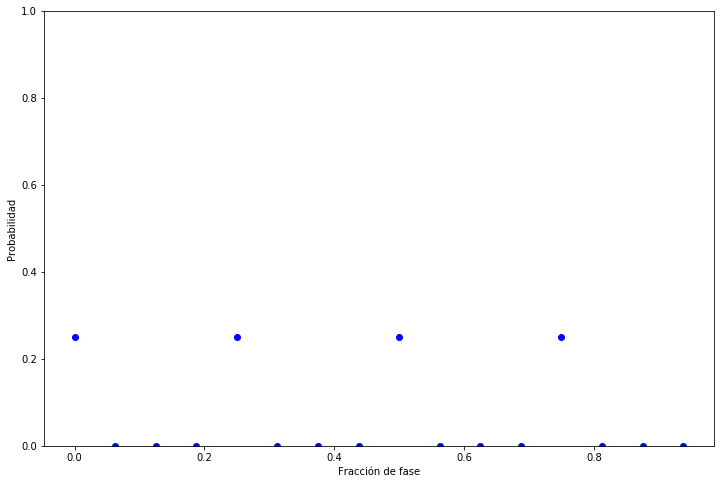
\includegraphics[width=0.9\linewidth]{img/ShorM15.png}
        \caption{Wolfram Mathematica}
    \end{subfigure}
    \begin{subfigure}[m]{0.45\textwidth}
        \centering
        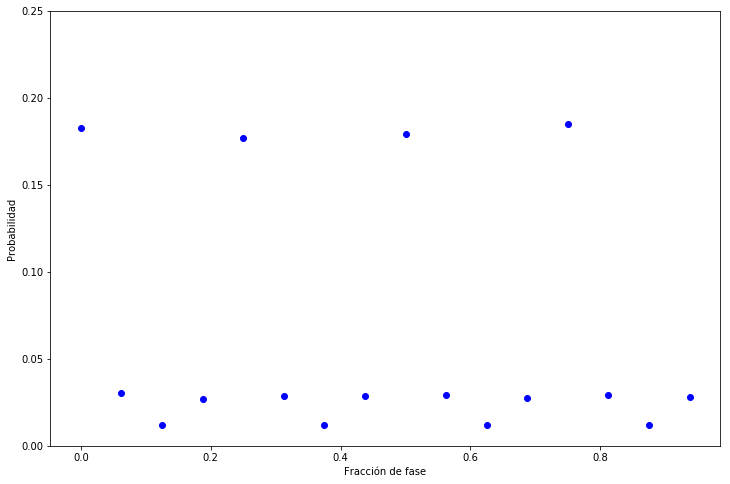
\includegraphics[width=0.9\linewidth]{img/shorlossless.png}
        \caption{Python}
    \end{subfigure}
    \caption[Distribución de probabilidad en la estimación de fase del algoritmo de Shor sin pérdidas]{Distribución de probabilidad en la estimación de fase del algoritmo de Shor sin pérdidas}
    \label{fig:shor15}
\end{figure}

\begin{figure}[H]
    \centering
    \begin{subfigure}[m]{0.45\textwidth}
        \centering
        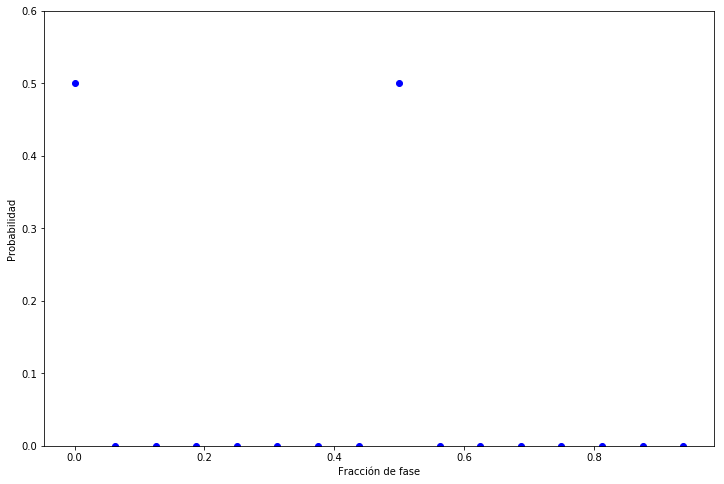
\includegraphics[width=0.9\linewidth]{img/ShorM8.png}
        \caption{Wolfram Mathematica}
    \end{subfigure}
    \begin{subfigure}[m]{0.45\textwidth}
        \centering
        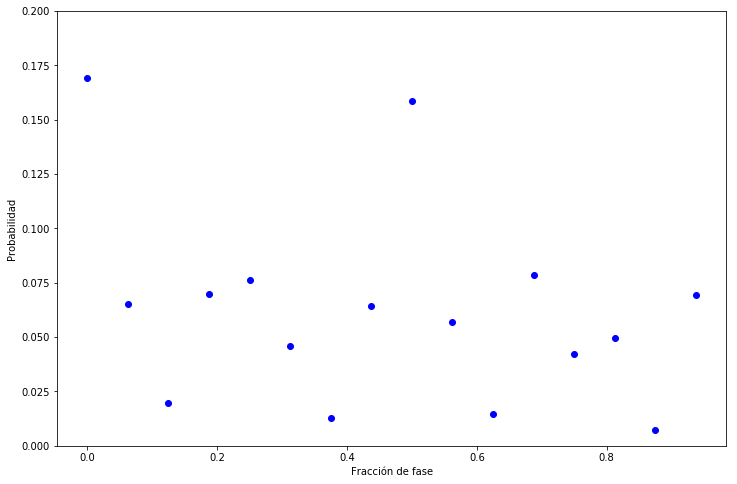
\includegraphics[width=0.9\linewidth]{img/shor2lossless.png}
        \caption{Python}
    \end{subfigure}
    \caption[Distribución de probabilidad en la estimación de fase del algoritmo de Shor sin pérdidas]{Distribución de probabilidad en la estimación de fase del algoritmo de Shor sin pérdidas}
    \label{fig:shor8}
\end{figure}

\end{frame}

\section{PageRank}

\begin{frame}
    \frametitle{PageRank}

    \begin{figure}[H]
    \begin{center}
    \begin{tabular}{c c c}
     \begin{tikzpicture}[->,>=stealth',shorten >=1pt,thick]
    \tikzset{VertexStyle/.style = {draw,circle,thick,
                                   minimum size=0.5cm,
                                   font=\bfseries},thick} 
    \Vertex[a = 90, d = 2.75]{1}  \Vertex[a = 162, d = 2.75]{2}
    \Vertex[a = 234, d = 2.75]{3} \Vertex[a = 306, d = 2.75]{4}
    \Vertex[a = 18, d = 2.75]{5}
    \Edge[label=$1$](2)(1)
    \Edge[label=$1$](1)(5)
    \Edge[label=$\frac{1}{2}$](3)(1)
    \Edge[label=$\frac{1}{2}$](3)(4)
    \Edge[label=$1$](4)(5)
    \tikzset{EdgeStyle/.style = {->, bend left}}
    \Edge[label=$1$](1)(3)
    \end{tikzpicture} 
    & \begin{tikzpicture}[->,>=stealth',shorten >=1pt,thick]
    \tikzset{VertexStyle/.style = {draw,circle,thick,
                                   minimum size=0.5cm,
                                   font=\bfseries},thick} 
    \Vertex[a = 90, d = 2.75]{1}  \Vertex[a = 162, d = 2.75]{2}
    \Vertex[a = 234, d = 2.75]{3} \Vertex[a = 306, d = 2.75]{4}
    \Vertex[a = 18, d = 2.75]{5}
    \Edge[label=$\frac{1}{10}$](5)(4)
    \Edge[label=$\frac{1}{10}$](4)(3)
    \Edge[label=$\frac{1}{10}$](3)(2)
    \Edge[label=$\frac{3}{5}$](2)(1)
    \Edge[label=$\frac{3}{5}$](1)(5)
    \Edge[label=$\frac{1}{10}$](1)(4)
    \Edge[label=$\frac{1}{10}$](4)(2)
    \Edge[label=$\frac{1}{10}$](2)(5)
    \Edge[label=$\frac{1}{10}$](5)(3)
    \Edge[label=$\frac{7}{20}$](3)(1)
    \Loop[dist=1cm,dir=NO,label=$\frac{1}{10}$,labelstyle=above](1)  
    \Loop[dist=1cm,dir=NOWE,label=$\frac{1}{10}$,labelstyle=above left](2)  
    \Loop[dist=1cm,dir=SOWE,label=$\frac{1}{10}$,labelstyle=below left](3)  
    \Loop[dist=1cm,dir=SOEA,label=$\frac{1}{10}$,labelstyle=below right](4)  
    \Loop[dist=1cm,dir=NOEA,label=$\frac{1}{10}$,labelstyle=above right](5)  
    \tikzset{EdgeStyle/.style = {->, bend right}}
    \Edge[label=$\frac{1}{10}$,labelstyle=above left](1)(2)
    \Edge[label=$\frac{1}{10}$,labelstyle=below left](2)(3)
    \Edge[label=$\frac{7}{20}$,labelstyle=below](3)(4)
    \Edge[label=$\frac{3}{5}$,labelstyle=below right](4)(5)
    \Edge[label=$\frac{1}{10}$,labelstyle=above right](5)(1)
    \Edge[label=$\frac{3}{5}$](1)(3)
    \Edge[label=$\frac{1}{10}$](3)(5)
    \Edge[label=$\frac{1}{10}$](5)(2)
    \Edge[label=$\frac{1}{10}$](2)(4)
    \Edge[label=$\frac{1}{10}$](4)(1)
    \end{tikzpicture} 
     \\
    (a) & (b)
    \end{tabular}
    \caption[Transformación de un grafo al crear la matriz de Google con $\alpha = \frac{1}{2}$]{Transformación de un grafo al crear la matriz de Google con $\alpha = \frac{1}{2}$: Grafo correspondiente a la matriz de adyacencia (a) de la red E (b) remendada de Google G con $\alpha=\frac{1}{2}$}
    \end{center}
    \end{figure}

\end{frame}

\begin{frame}
    \frametitle{Caminatas cuánticas}

    \begin{figure}[H]
    \begin{tabular}{c c}
    \begin{tikzpicture}[,>=stealth',shorten >=1pt,thick]
    \tikzset{VertexStyle/.style = {draw,circle,thick,
                                   minimum size=1cm,
                                   font=\bfseries},thick} 
    \Vertex[x = -3, y = 0]{-2}  \Vertex[x = -1.5, y = 0]{-1}
    \Vertex[x = 0, y = 0]{0} \Vertex[x = 1.5, y = 0]{1}
    \Vertex[x = 3, y = 0]{2}
    \Edges(-2,-1,0,1,2)
    \end{tikzpicture} &
    \begin{tikzpicture}[,>=stealth',shorten >=1pt,thick]
    \tikzset{VertexStyle/.style = {draw,circle,thick,
                                   minimum size=1cm,
                                   font=\scriptsize\bfseries},thick} 
    \Vertex[x = -3, y = 0, L = $\ket{-2}$]{-2}  \Vertex[x = -1.5, y = 0, L = $\ket{-1}$]{-1}
    \Vertex[x = 0, y = 0, L = $\ket{0}$]{0} \Vertex[x = 1.5, y = 0, L = $\ket{1}$]{1}
    \Vertex[x = 3, y = 0, L = $\ket{2}$]{2}
    \Edges(-2,-1,0,1,2)
    \end{tikzpicture}
    \end{tabular}
    \end{figure}

\end{frame}

\begin{frame}
    \frametitle{Caminatas cuánticas de Szegedy}

    \begin{figure}[h]
    \begin{tabular}{c c c}
    \begin{tikzpicture}[->,>=stealth',shorten >=1pt,thick]
    \SetGraphUnit{2} 
    \tikzset{VertexStyle/.style = {draw,circle,thick,
                                   minimum size=0.5cm,
                                   font=\bfseries},thick} 
    \Vertex{1} \SOWE(1){2} \SOEA(2){3} \SOEA(1){4} 
    \Edges(1,2,3) \Edge(1)(4)

    \tikzset{EdgeStyle/.style = {->, bend left}}
    \Edge(3)(2)
    % it's possible with \Edge but Tikz's syntax is allowed too.
    \end{tikzpicture} 
    &
    \begin{tikzpicture}[->,>=stealth',shorten >=1pt,thick]
    \tikzset{VertexStyle/.style = {draw,circle,thick,
                                   minimum size=0.5cm,
                                   font=\bfseries},thick} 
    \Vertex[x = 0, y = 0]{1a} \Vertex[x = 0, y = -1]{2a}
    \Vertex[x = 0, y = -2]{3a}\Vertex[x = 0, y = -3]{4a}
    \Vertex[x = 3, y = 0]{1b} \Vertex[x = 3, y = -1]{2b}
    \Vertex[x = 3, y = -2]{3b}\Vertex[x = 3, y = -3]{4b}
    \Edge(1a)(2b)	\Edge(1a)(3b)	\Edge(2a)(4b)
    \Edge(4a)(2b)
    \end{tikzpicture}
    &
    \begin{tikzpicture}[->,>=stealth',shorten >=1pt,thick]
    \tikzset{VertexStyle/.style = {draw,circle,thick,
                                   minimum size=0.5cm,
                                   font=\bfseries},thick} 
    \Vertex[x = 0, y = 0]{1a} \Vertex[x = 0, y = -1]{2a}
    \Vertex[x = 0, y = -2]{3a}\Vertex[x = 0, y = -3]{4a}
    \Vertex[x = 3, y = 0]{1b} \Vertex[x = 3, y = -1]{2b}
    \Vertex[x = 3, y = -2]{3b}\Vertex[x = 3, y = -3]{4b}
    \Edge(2b)(1a)	\Edge(3b)(1a)	\Edge(4b)(2a)
    \Edge(4b)(1a)
    \end{tikzpicture}
    \end{tabular}
    \end{figure}

\end{frame}

\begin{frame}
    \frametitle{PageRank cuántico}


\begin{equation}
    I_q(P_i,m) =  Tr((\mathds{1} \otimes \ketbra{i}{i}) U^m \ketbra{\psi_0} U^{\dagger m}) .
\end{equation}

\begin{equation}
    \ket{\psi_0} = \frac{1}{\sqrt{N}} \sum\limits_i \ket{\psi_i} .
\end{equation}

\begin{equation}
    \langle I_q(P_i) \rangle = \frac{1}{M} \sum\limits_{m=0}^{M-1} I_q(P_i,m)
\end{equation}

\end{frame}

\begin{frame}
    \frametitle{Circuitos de Loke}

\begin{figure}[H]
\[\Qcircuit @C=1.4em @R=1.8em {
        & \targ     & \qw      & \qw \\
        & \ctrl{-1} & \gate{X} & \qw \\
} 
\]
\caption[Operador de permutación]{Operador de permutación $T$}
\label{fig:T}
\end{figure}

\begin{figure}[H]
\[\Qcircuit @C=1.4em @R=1.8em {
        \lstick{\text{Registro 1}}& {/}\qw & \ctrl{1}   & \ctrl{1}           & \qw      & \ctrl{1}   & \ctrl{1}           & \qswap     & \qw \\
        \lstick{\text{Registro 2}}& {/}\qw & \gate{T_i} & \gate{K_b^\dagger} & \gate{D} & \gate{K_b} & \gate{T_i^\dagger} & \qswap\qwx & \qw \\
& & & & \rstick{\hspace{-13pt} 2 \text{ veces}}
\gategroup{2}{3}{2}{8}{1.5em}{_\}}
} 
\]
\caption[Circuito de Loke \cite{loke} para las caminatas cuánticas de Szegedy]{Circuito de Loke para las caminatas cuánticas de Szegedy}
\label{fig:lokecircuit}
\end{figure}

\begin{figure}[H]
\[\Qcircuit @C=1.4em @R=1.8em {
& \gate{Ry(\theta_{00})} & \ctrlo{1}               & \ctrl{1}               & \qw \\
& \qw                    & \gate{Ry(\theta_{10})}  & \gate{Ry(\theta_{11})} & \qw \\
} \]
\caption{Circuito de $K_i$}
\end{figure}

\begin{align}
    \theta_{00} &= 2 \cos^{-1}\left(\sqrt{G_1 + G_2}\right) \\
    \theta_{10} &= 2 \cos^{-1}\left(\sqrt{\frac{G_1}{G_1 + G_2}}\right) \\
    \theta_{11} &= 2 \cos^{-1}\left(\sqrt{\frac{G_3}{1 - (G_1 + G_2)}}\right) .
\end{align}

\end{frame}

\begin{frame}
    \frametitle{Simulaciones del algoritmo de PageRank cuántico}


\begin{figure}[H]
    \centering
    \begin{tikzpicture}[->,>=stealth',shorten >=1pt,thick]
    \SetGraphUnit{2} 
    \tikzset{VertexStyle/.style = {draw,circle,thick,
                                   minimum size=0.5cm,
                                   font=\bfseries},thick} 
    \Vertex{1} \NO(1){2} \SOEA(1){3} \SOWE(1){4} 
    \Edge(1)(2)
    \Edge(1)(3)
    \Edge(1)(4)
    
    \tikzset{EdgeStyle/.style = {->, bend left}}
    \Edge(2)(1)
    \Edge(3)(1)
    \Edge(4)(1)
    \end{tikzpicture} 
    \caption[Grafo estrella]{Grafo estrella}
    \label{fig:star}
\end{figure}

\begin{equation}
    A =
    \begin{pmatrix}
        0 & 1 & 1 & 1 \\
        1 & 0 & 0 & 0 \\
        1 & 0 & 0 & 0 \\
        1 & 0 & 0 & 0
    \end{pmatrix}
\end{equation}

\begin{equation}
    E = 
    \begin{pmatrix}
        0 & 1 & 1 & 1 \\
        \frac{1}{3} & 0 & 0 & 0 \\
        \frac{1}{3} & 0 & 0 & 0 \\
        \frac{1}{3} & 0 & 0 & 0
    \end{pmatrix}
\end{equation}

\begin{equation}
    G =
    \begin{pmatrix}
        \frac{3}{80} & \frac{71}{80} & \frac{71}{80} & \frac{71}{80} \\
        \frac{77}{240} & \frac{3}{80} & \frac{3}{80} & \frac{3}{80} \\
        \frac{77}{240} & \frac{3}{80} & \frac{3}{80} & \frac{3}{80} \\
        \frac{77}{240} & \frac{3}{80} & \frac{3}{80} & \frac{3}{80}
    \end{pmatrix}
\end{equation}

\begin{figure}[H]
\[\Qcircuit @C=1.4em @R=1.8em {
& \gate{Ry(1.85806)} & \ctrlo{1}           & \ctrl{1}          & \qw \\
& \qw                & \gate{Ry(2.48274)}  & \gate{Ry(1.5708)} & \qw \\
} \]
\caption{Circuito de $K_1$ para el grafo estrella}
\label{fig:starkb1}
\end{figure}

\begin{figure}[H]
\[\Qcircuit @C=1.4em @R=1.8em {
& \gate{Ry(0.554811)} & \ctrlo{1}            & \ctrl{1}          & \qw \\
& \qw                 & \gate{Ry(0.405465)}  & \gate{Ry(1.5708)} & \qw \\
} \]
\caption{Circuito de $K_2$ para el grafo estrella}
\label{fig:starkb2}
\end{figure}

\begin{figure}[H]
\[\Qcircuit @C=1.4em @R=1.8em {
& \ctrlo{1}                   & \qw                 & \ctrlo{1}           & \qw \\
& \ctrlo{1}                   & \qw                 & \ctrlo{1}           & \qw \\
& \multigate{1}{K_1^\dagger} & \multigate{1}{K_1} & \multigate{1}{K_2} & \qw \\
& \ghost{K_1^\dagger}        & \ghost{K_1}        & \ghost{K_2}        & \qw \\
} 
\]
\caption[$K_b$ del grafo estrella]{$K_b$ del grafo estrella}
\label{fig:starkb}
\end{figure}

\begin{figure}[H]
\[\Qcircuit @C=1.4em @R=1.8em {
& \gate{I} & \qw \\
& \gate{I} & \qw \\
& \gate{I} & \qw \\
& \gate{I} & \qw \\
} 
\]
\caption[$T$ del grafo estrella]{$T$ del grafo estrella}
\label{fig:starT}
\end{figure}

\begin{figure}[H]
\[\Qcircuit @C=1.4em @R=1.8em {
& \gate{H} & \multigate{3}{K_b} & \qw \\
& \gate{H} & \ghost{K_b}        & \qw \\
& \qw      & \ghost{K_b}        & \qw \\
& \qw      & \ghost{K_b}        & \qw \\
} 
\]
\caption{Preparación del estado inicial para la caminata en el grafo estrella}
\label{fig:starinit}
\end{figure}

\begin{figure}[H]
\[ \Qcircuit @C=1.4em @R=1.8em {
\lstick{\ket{0}} & {/^4} \qw & \gate{Init} & \gate{K_b^\dagger} & \gate{D} & \gate{K_b} & \gate{SWAP} & \meter & \cw \\
                 & & & & \rstick{2m \text{ veces}}
\gategroup{1}{4}{1}{7}{1.3em}{_\}}
} \]
\caption{Circuito del PageRank cuántico  del grafo estrella}
\label{fig:lokestar}
\end{figure}

\begin{figure}[H]
    \centering
    \begin{subfigure}[m]{0.45\textwidth}
        \centering
        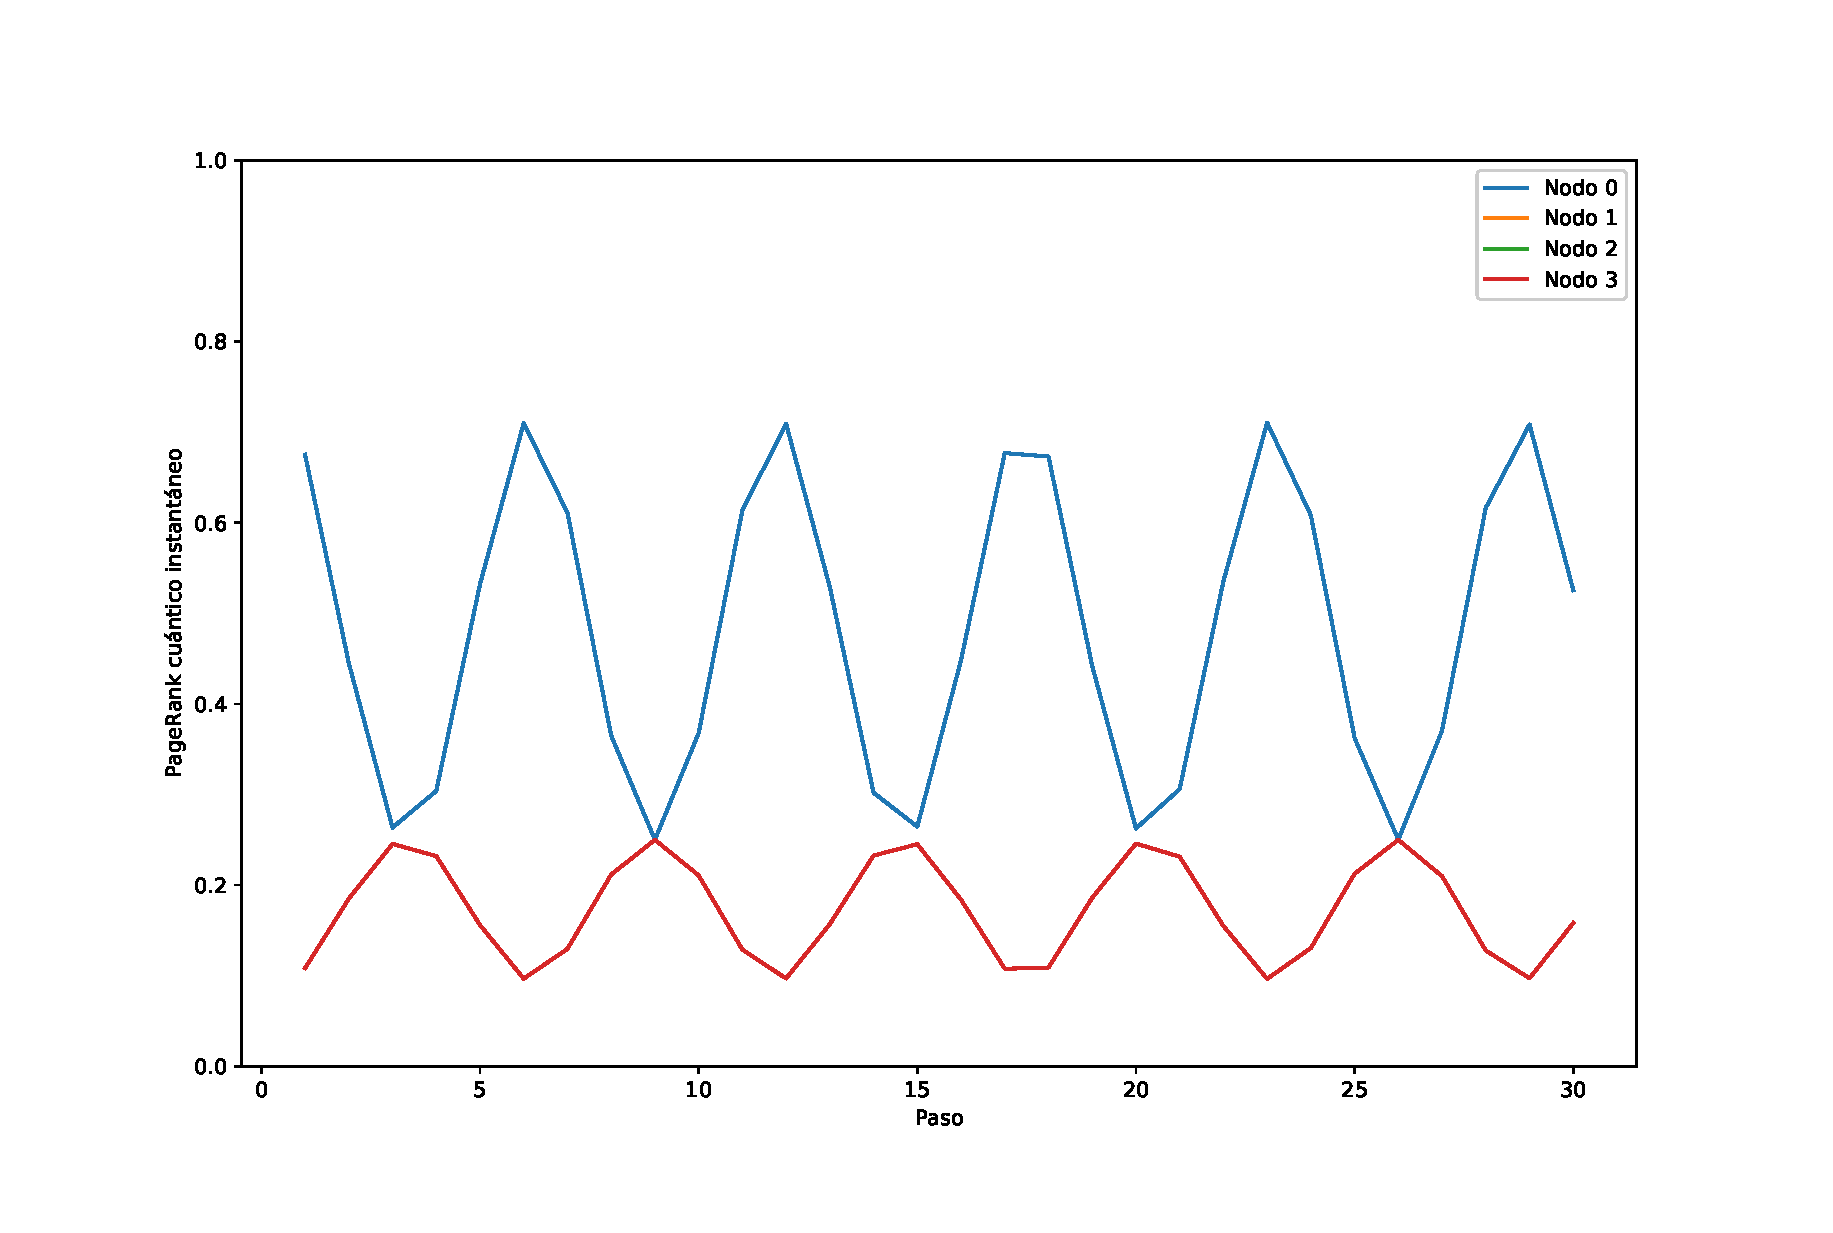
\includegraphics[width=0.9\linewidth]{img/star-inst-M.eps}
        \caption{Wolfram Mathematica}
    \end{subfigure}
    \begin{subfigure}[m]{0.45\textwidth}
        \centering
        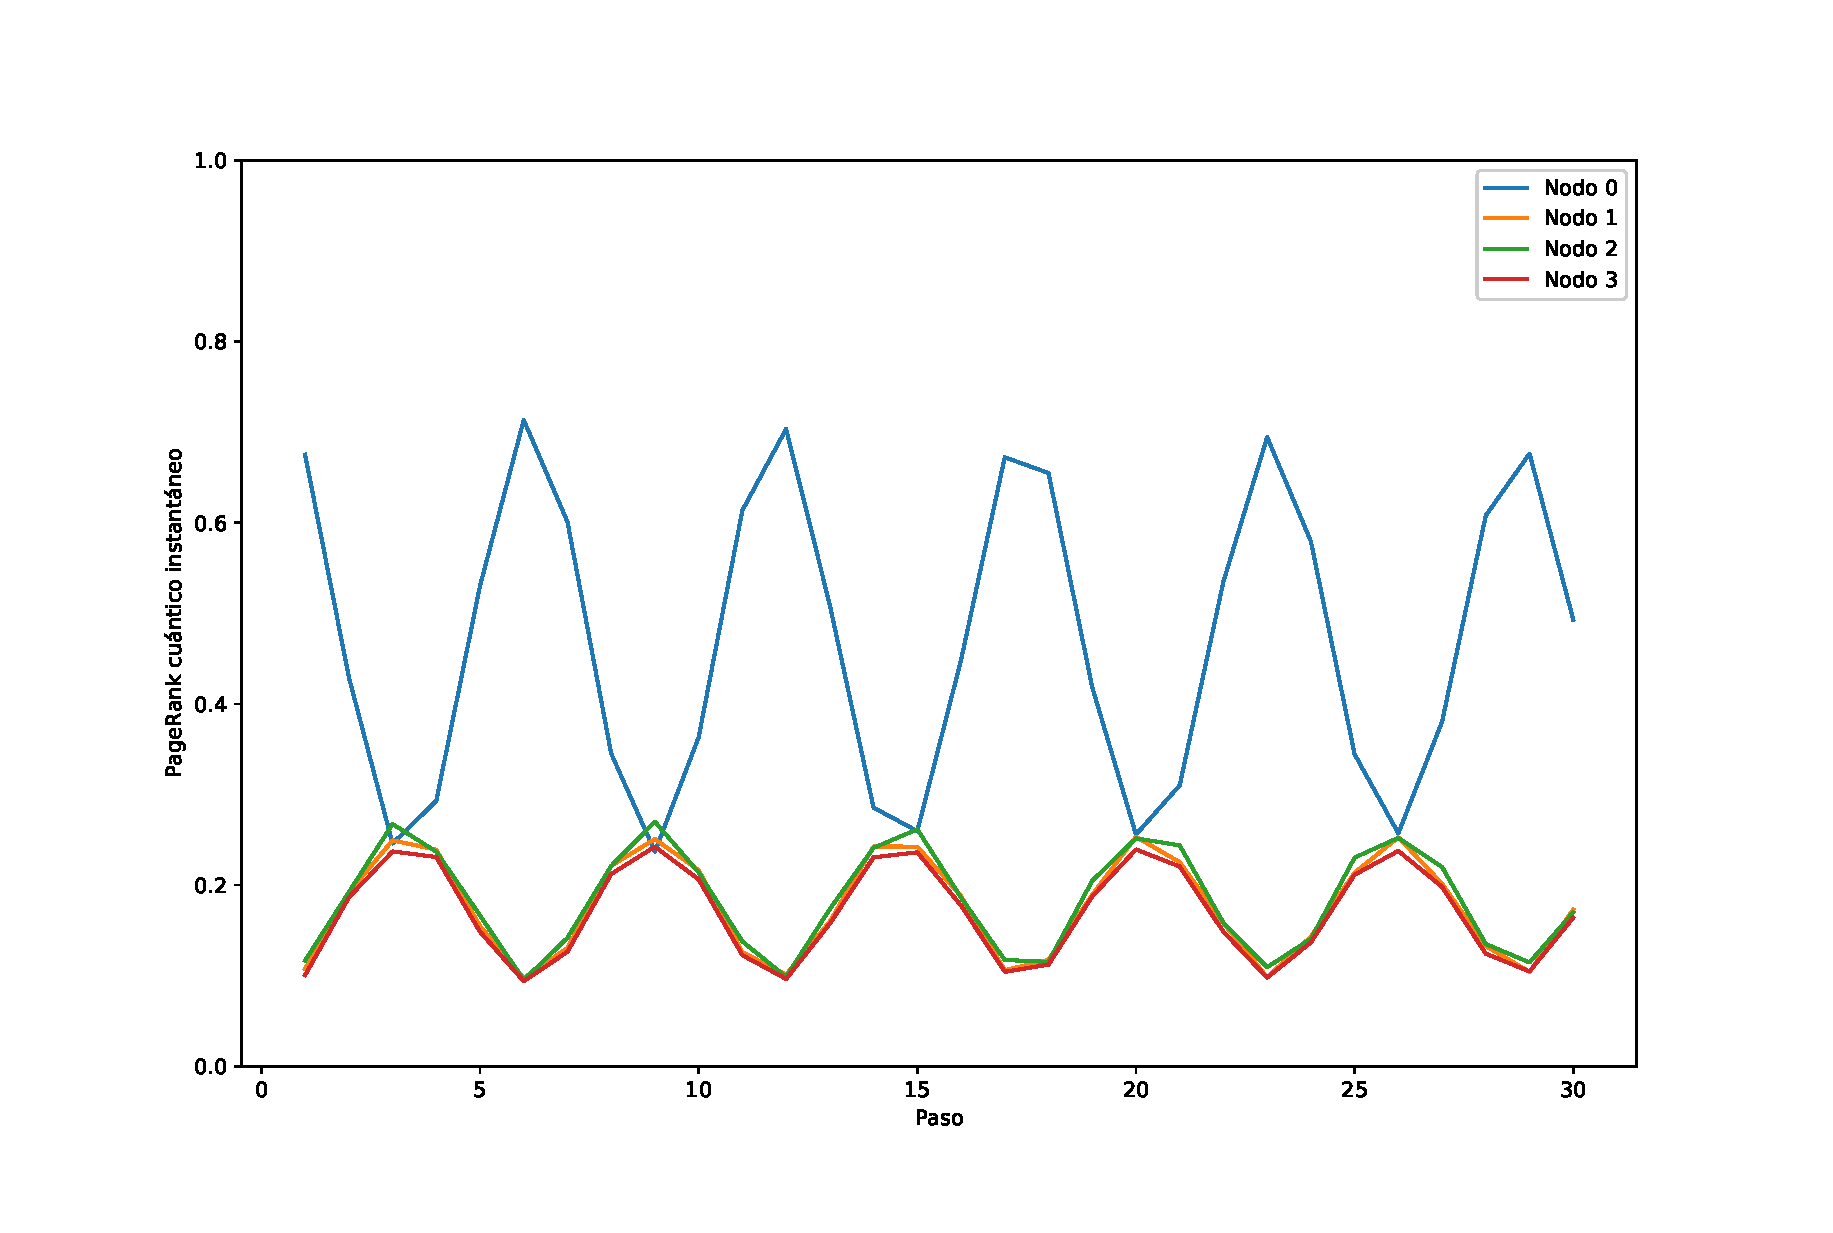
\includegraphics[width=0.9\linewidth]{img/star-inst-lossless.eps}
        \caption{Python}
    \end{subfigure}
    \caption[PageRank cuántico instantáneo del grafo estrella sin pérdidas]{PageRank cuántico instantáneo del grafo estrella sin pérdidas}
    \label{fig:inststarlossless}
\end{figure}

\begin{figure}[H]
    \centering
    \begin{subfigure}[m]{0.45\textwidth}
        \centering
        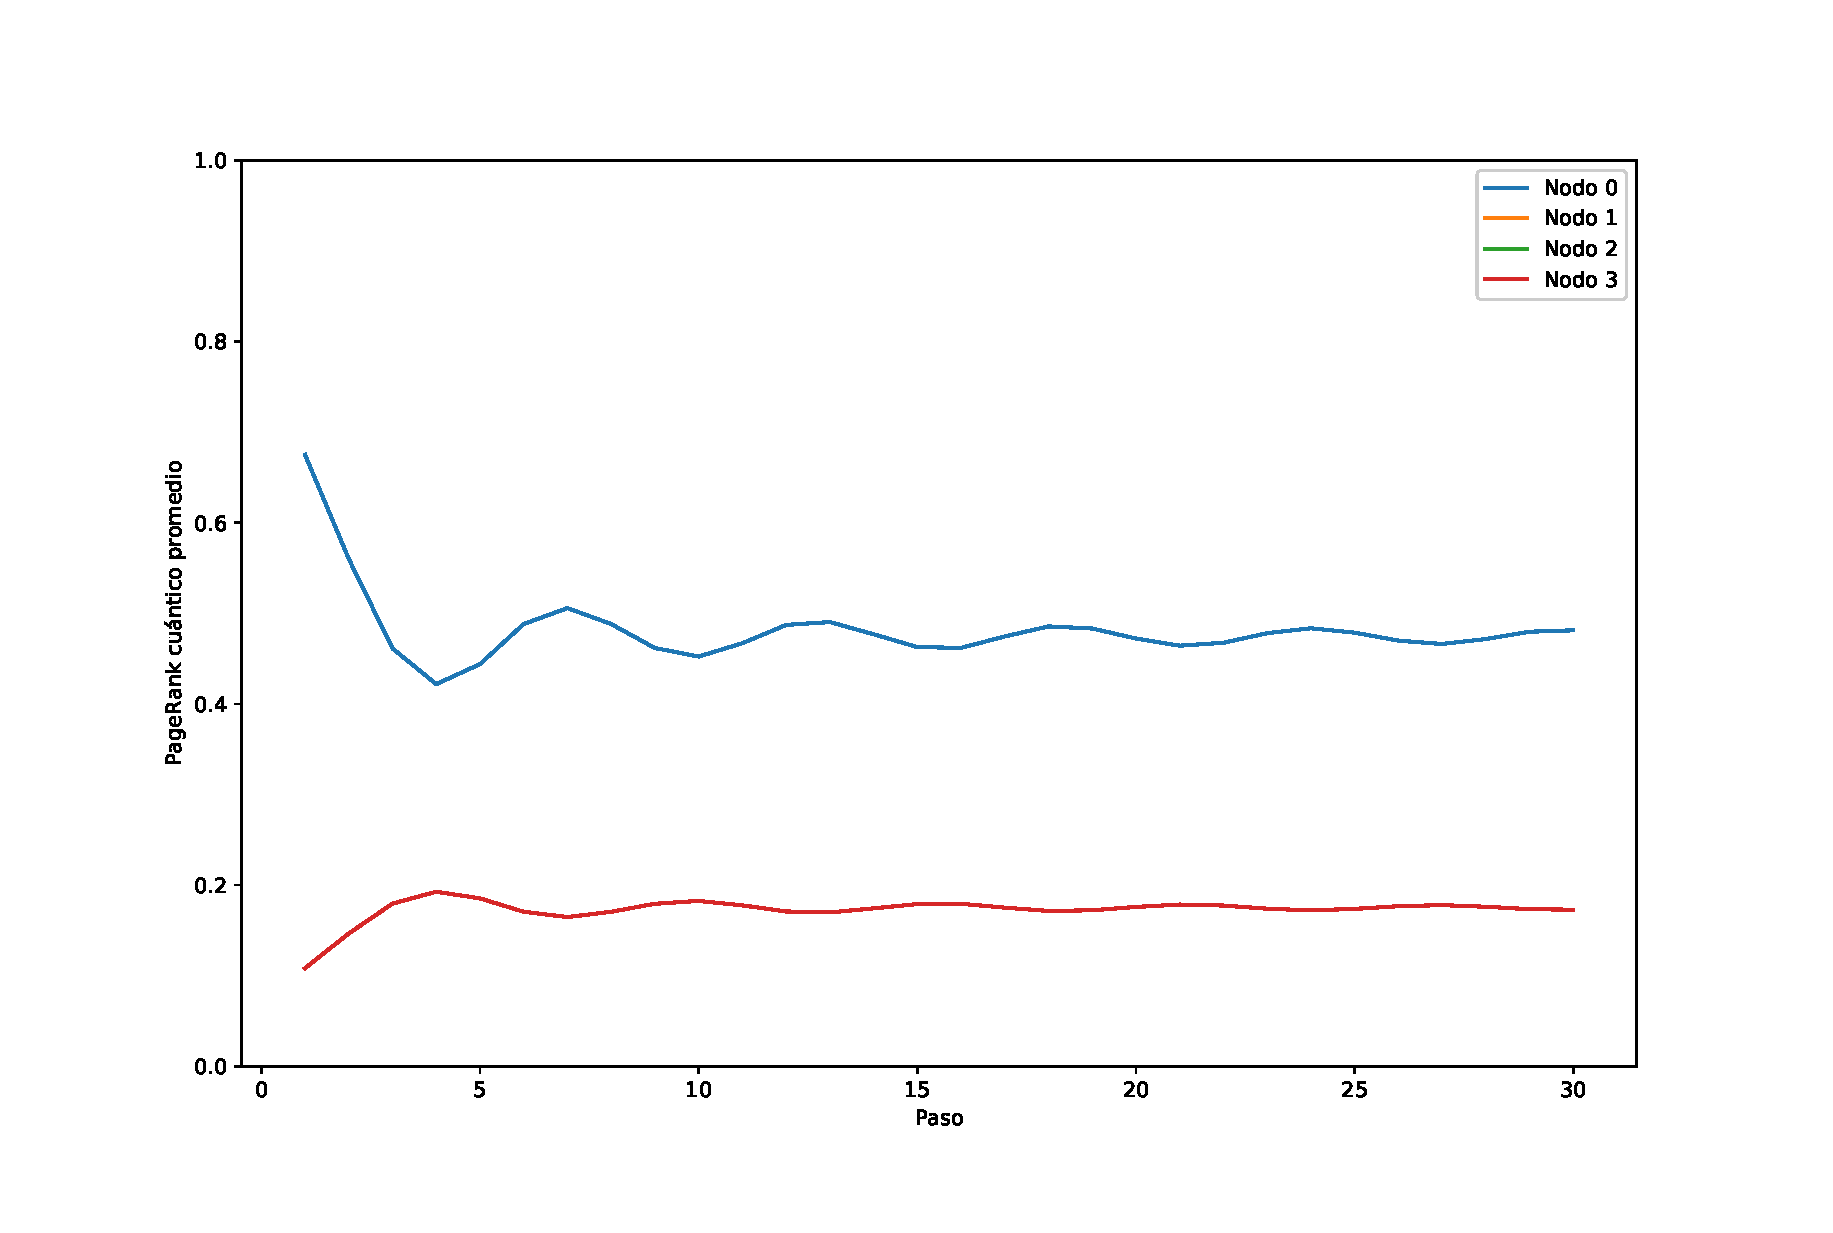
\includegraphics[width=0.9\linewidth]{img/star-mean-M.eps}
        \caption{Wolfram Mathematica}
    \end{subfigure}
    \begin{subfigure}[m]{0.45\textwidth}
        \centering
        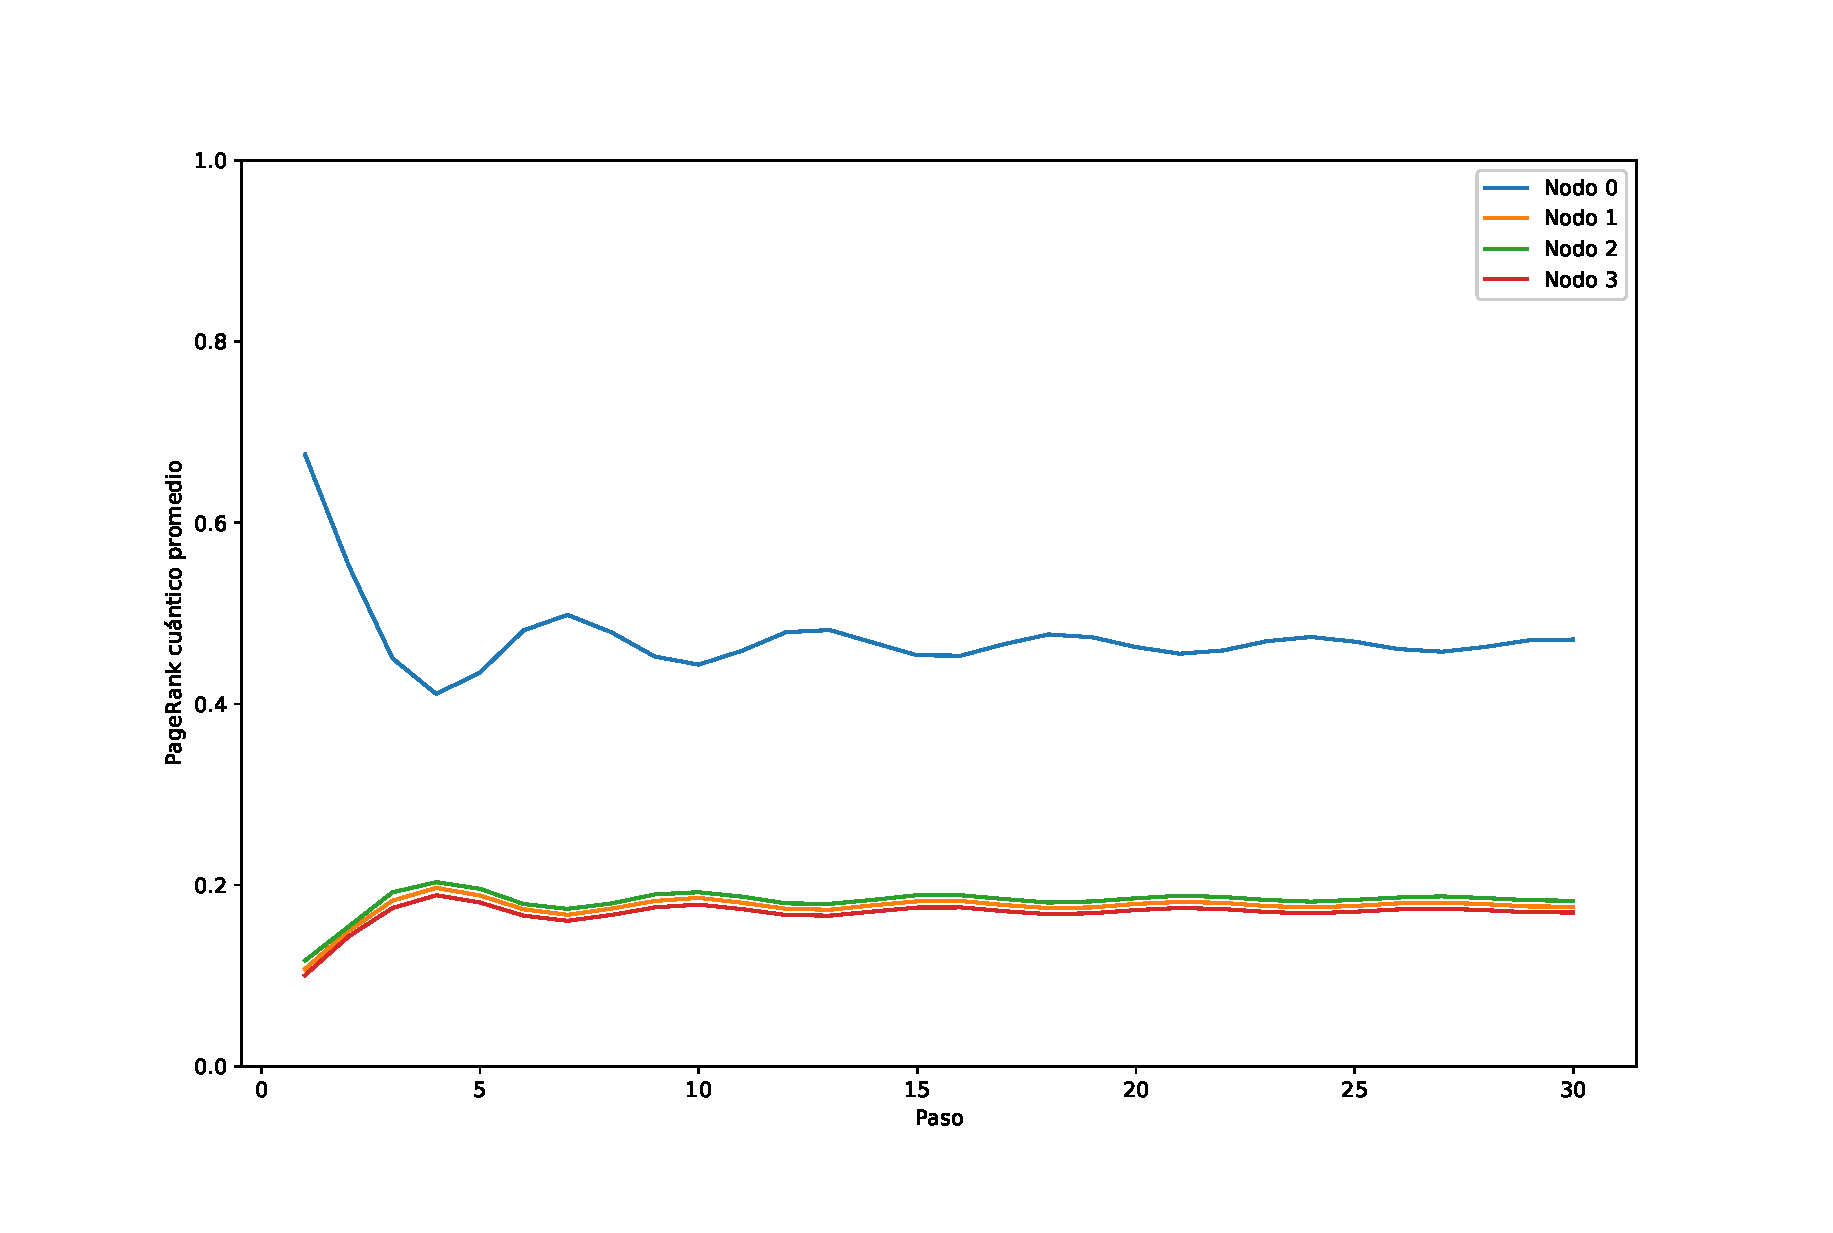
\includegraphics[width=0.9\linewidth]{img/star-mean-lossless.eps}
        \caption{Python}
    \end{subfigure}
    \caption[PageRank cuántico promedio del grafo estrella sin pérdidas]{PageRank cuántico promedio del grafo estrella sin pérdidas}
    \label{fig:meanstarlossless}
\end{figure}

\begin{figure}[H]
    \centering
    \begin{subfigure}[m]{0.45\textwidth}
        \centering
        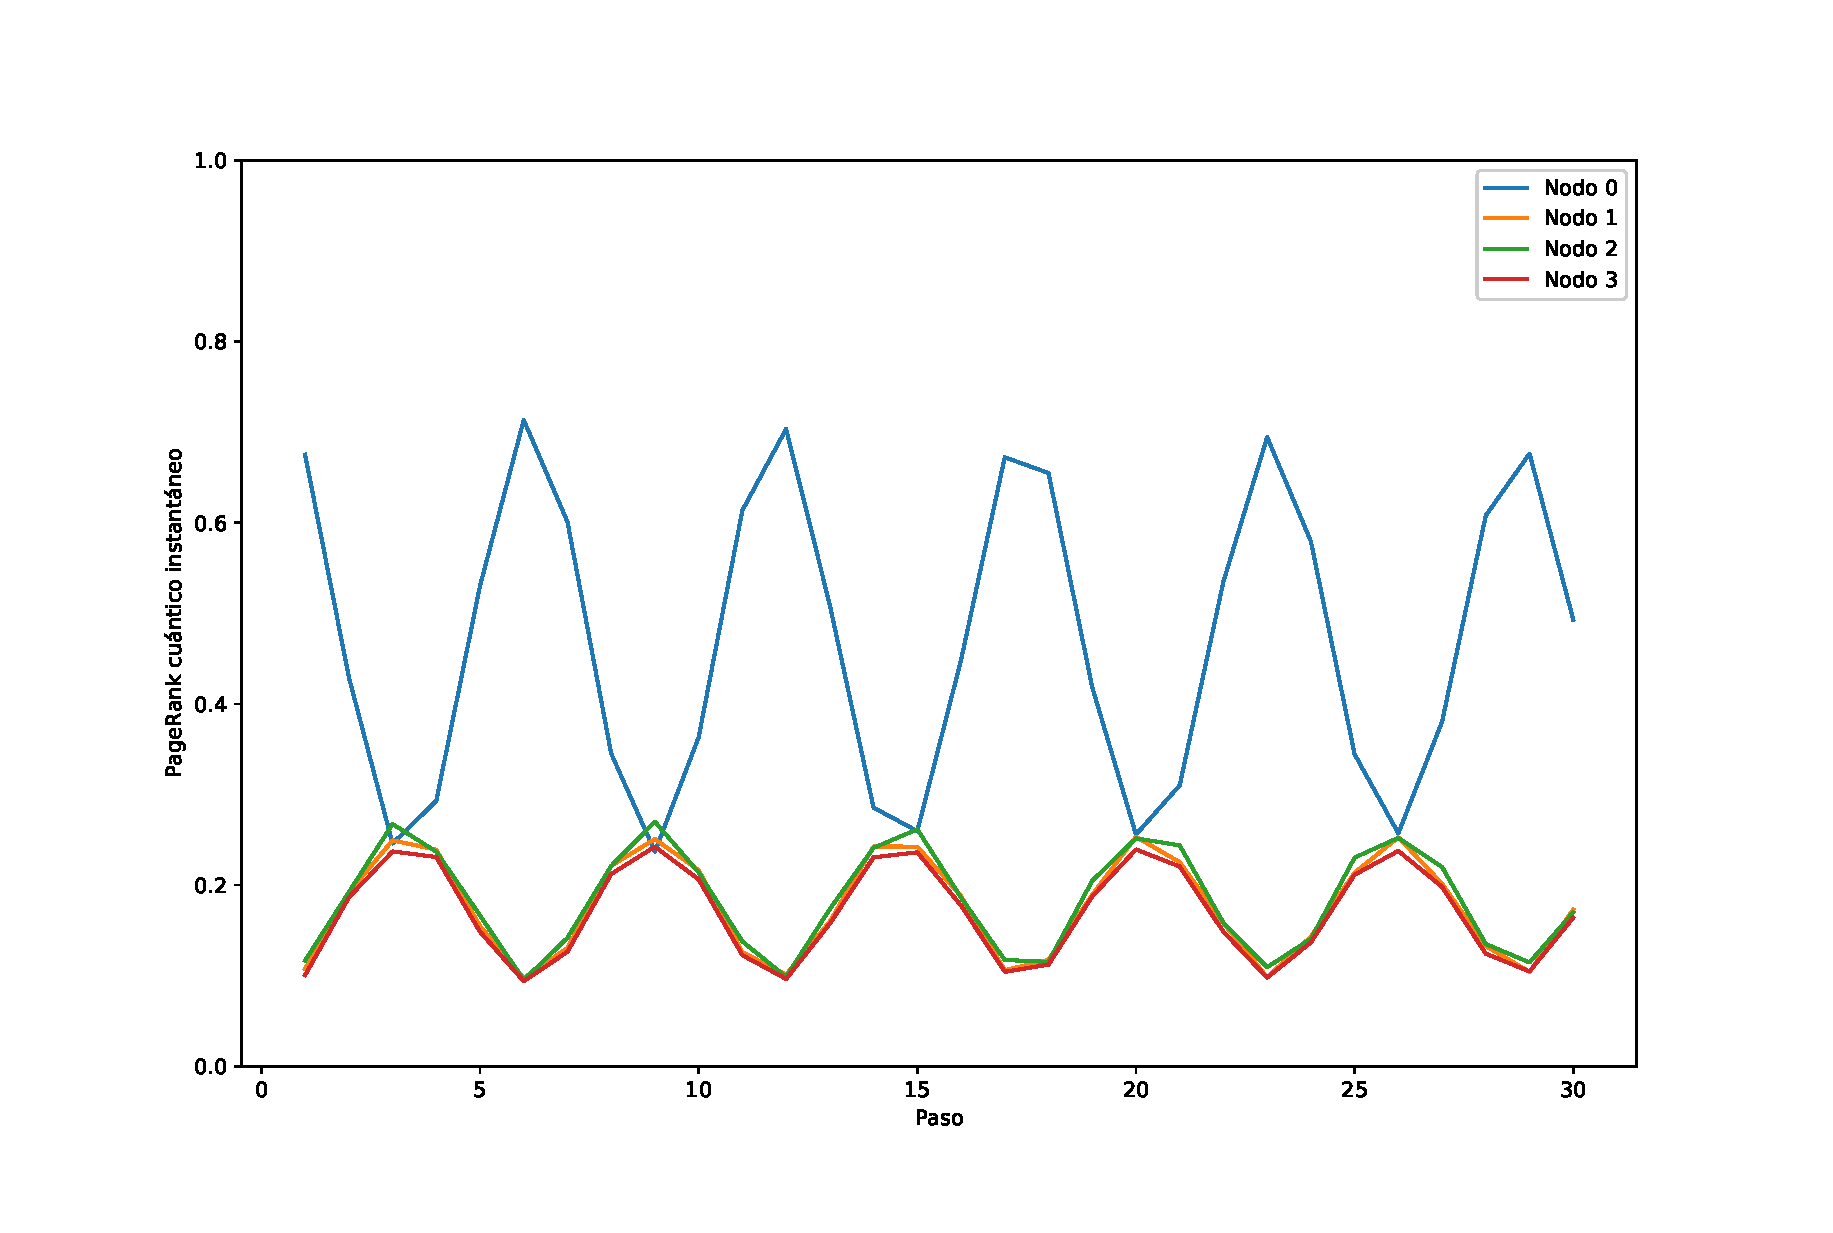
\includegraphics[width=0.9\linewidth]{img/star-inst-lossless.eps}
        \caption{Sin relajación}
    \end{subfigure}
    \begin{subfigure}[m]{0.45\textwidth}
        \centering
        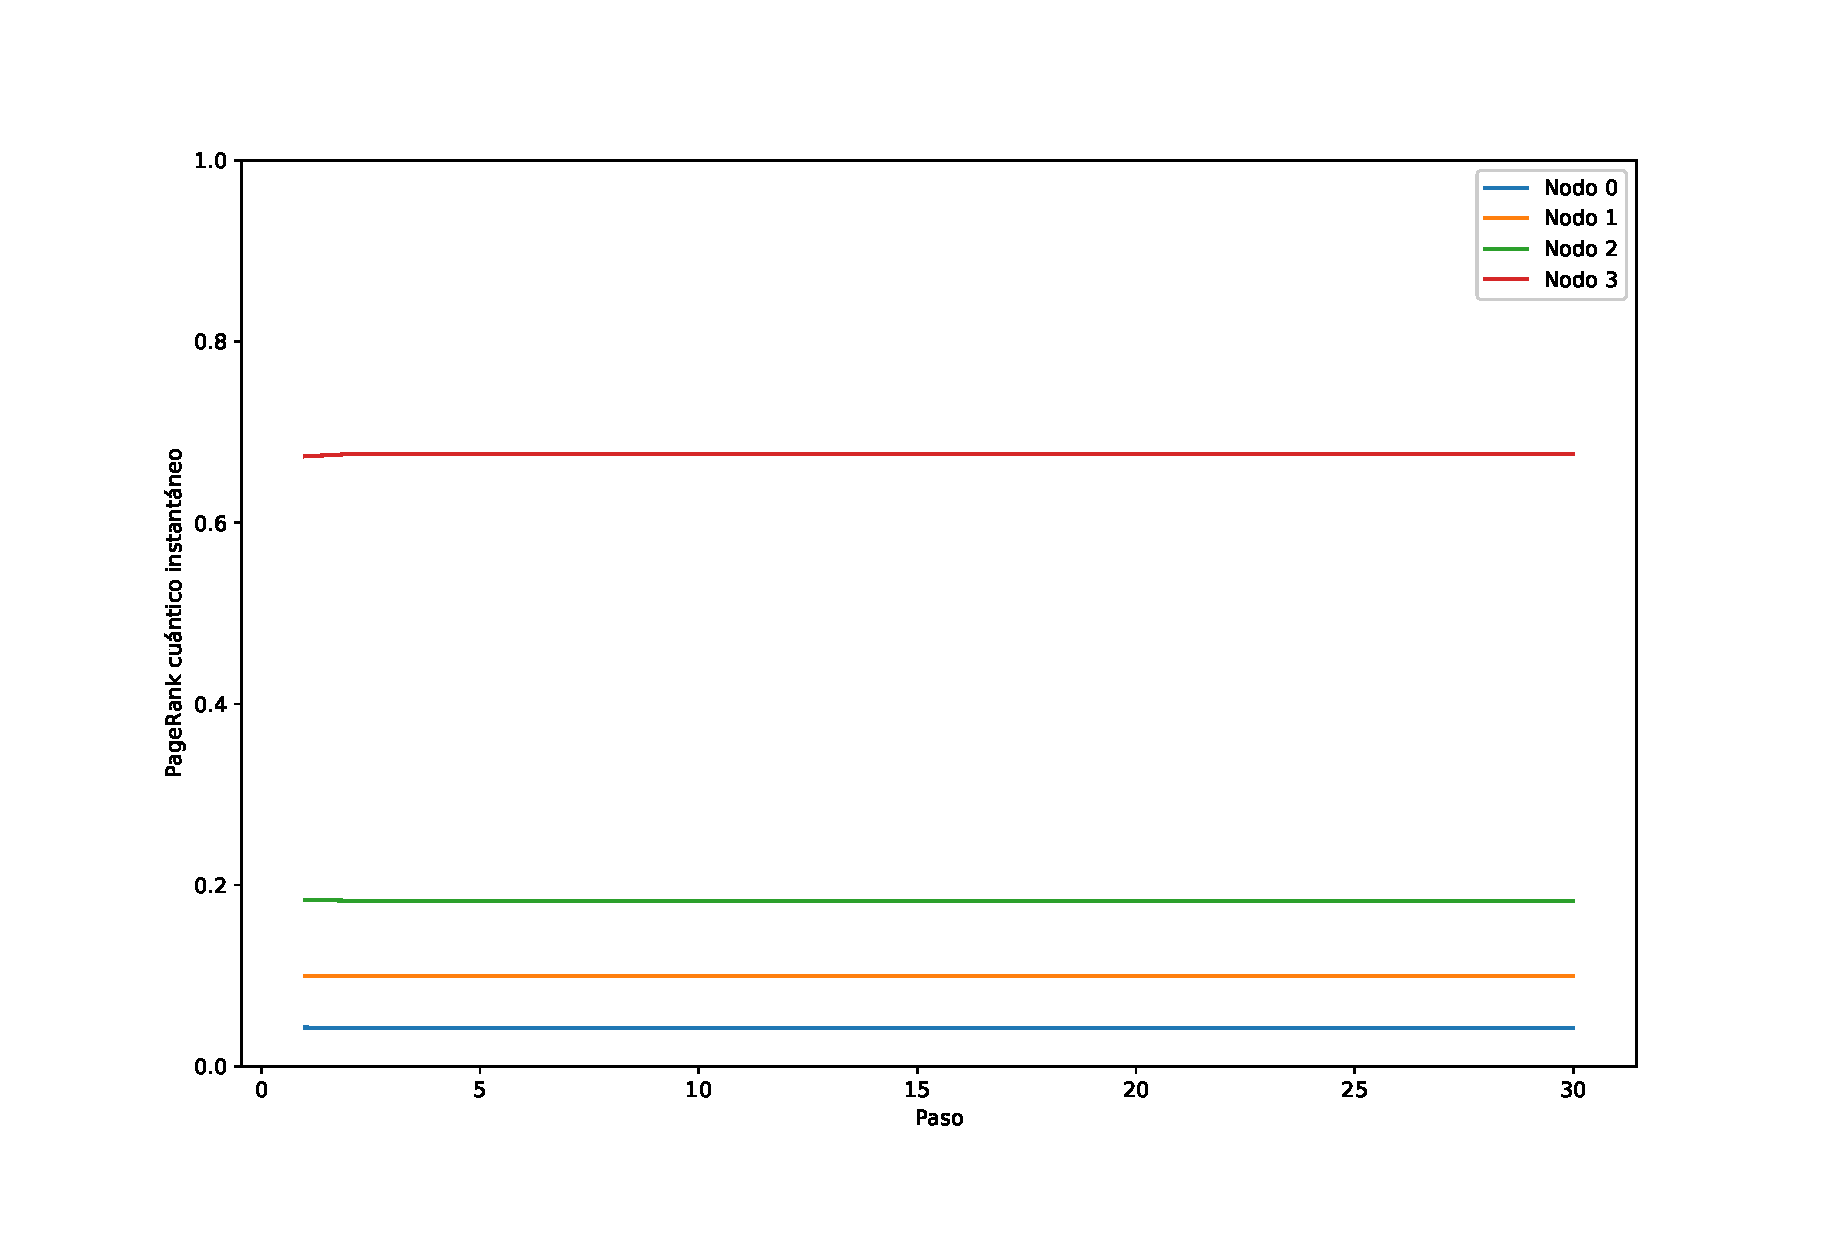
\includegraphics[width=0.9\linewidth]{img/star-inst-lossy.eps}
        \caption{Con relajación}
    \end{subfigure}
    \caption[PageRank cuántico instantaneo del grafo estrella con y sin pérdidas]{PageRank cuántico instantaneo del grafo estrella con y sin pérdidas}
    \label{fig:inststarlossy}
\end{figure}

\begin{figure}[H]
    \centering
    \begin{subfigure}[m]{0.9\textwidth}
        \centering
        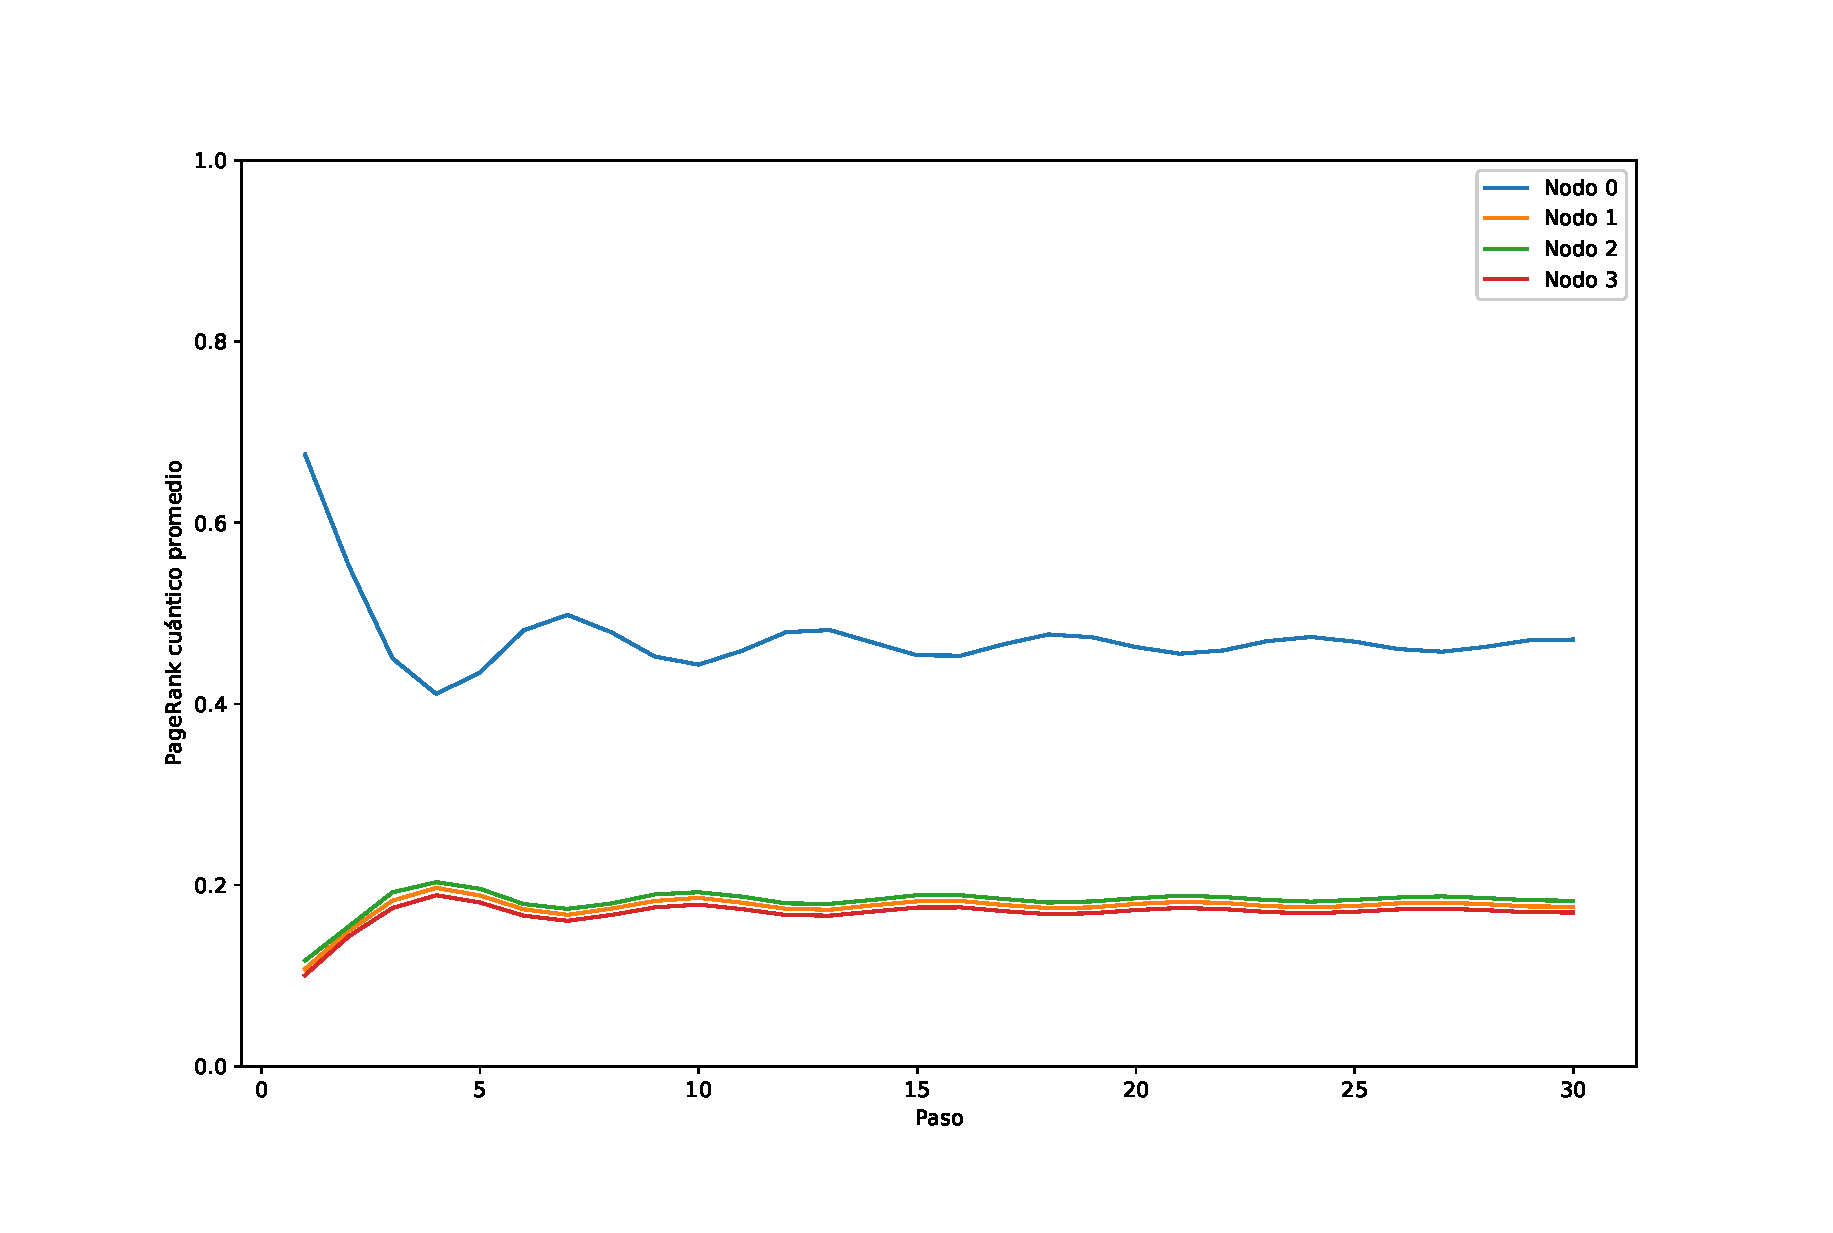
\includegraphics[width=0.9\linewidth]{img/star-mean-lossless.eps}
        \caption{Sin relajación}
    \end{subfigure}
    \begin{subfigure}[m]{0.9\textwidth}
        \centering
        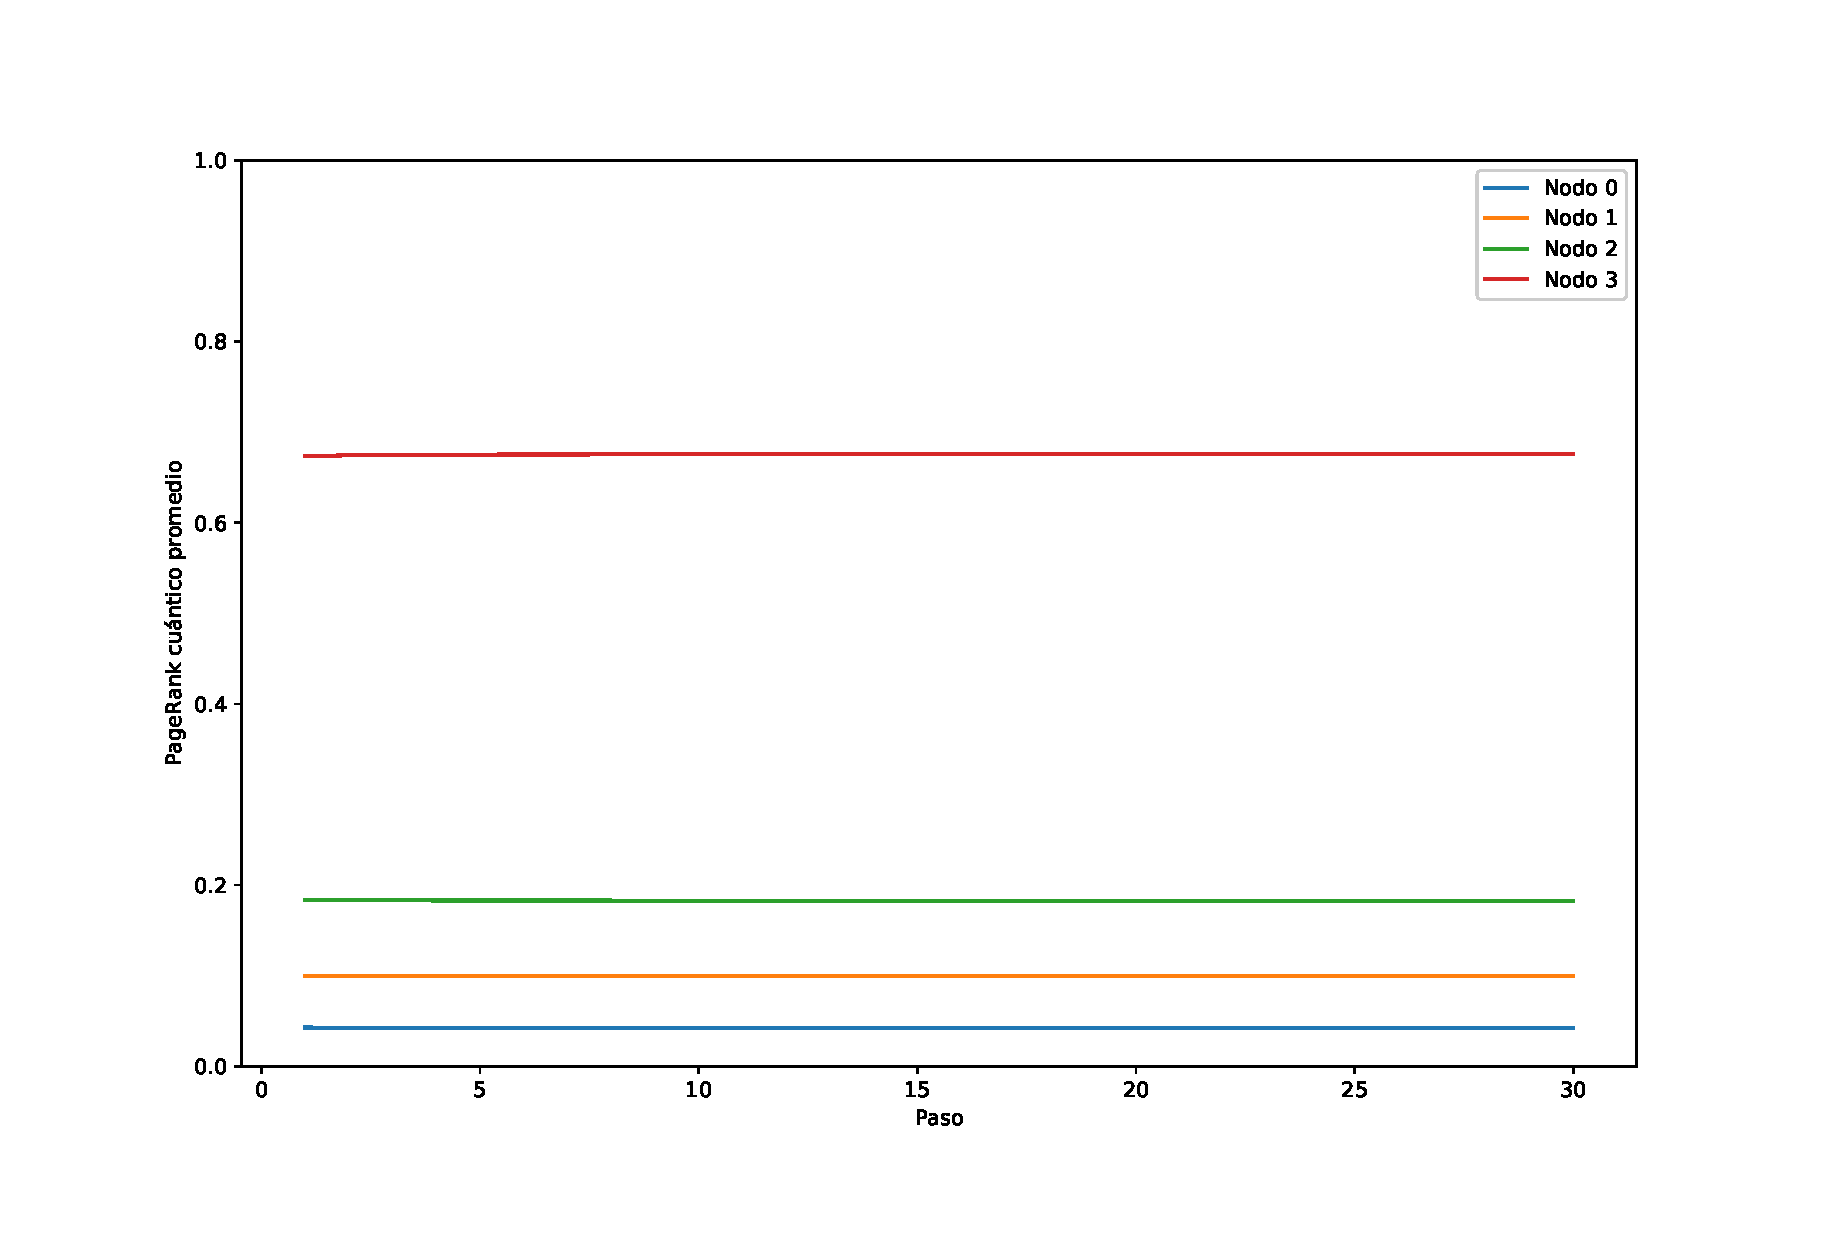
\includegraphics[width=0.9\linewidth]{img/star-mean-lossy.eps}
        \caption{Con relajación}
    \end{subfigure}
    \caption[PageRank cuántico promedio del grafo estrella con y sin pérdidas]{PageRank cuántico promedio del grafo estrella con y sin pérdidas}
    \label{fig:meanstarlossy}
\end{figure}








\begin{figure}[H]
    \centering
    \begin{tikzpicture}[->,>=stealth',shorten >=1pt,thick]
    \SetGraphUnit{2} 
    \tikzset{VertexStyle/.style = {draw,circle,thick,
                                   minimum size=0.5cm,
                                   font=\bfseries},thick} 
    \Vertex{4} \NO(4){1} \SOEA(4){2} \SOWE(4){3} 
    \Edge(1)(4)
    \Edge(2)(4)
    \Edge(3)(4)
    \Edges(3,2,1,3)
    \tikzset{EdgeStyle/.style = {->, bend left}}
    \Edges(1,2,3,1)
    \end{tikzpicture} 
    \caption[Grafo corona]{Grafo corona}
    \label{fig:crown}
\end{figure}

\begin{equation}
    A =
    \begin{pmatrix}
        0 & 1 & 1 & 0 \\
        1 & 0 & 1 & 0 \\
        1 & 1 & 0 & 0 \\
        1 & 1 & 1 & 0 \\
    \end{pmatrix}
\end{equation}

\begin{equation}
    E =
    \begin{pmatrix}
        0 & \frac{1}{3} & \frac{1}{3} & \frac{1}{4} \\
        \frac{1}{3} & 0 & \frac{1}{3} & \frac{1}{4} \\
        \frac{1}{3} & \frac{1}{3} & 0 & \frac{1}{4} \\
        \frac{1}{3} & \frac{1}{3} & \frac{1}{3} & \frac{1}{4} \\
    \end{pmatrix}
\end{equation}

\begin{equation}
    G =
    \begin{pmatrix}
        \frac{3}{80} & \frac{77}{240} & \frac{77}{240} & \frac{1}{4} \\
        \frac{77}{240} & \frac{3}{80} & \frac{77}{240} & \frac{1}{4} \\
        \frac{77}{240} & \frac{77}{240} & \frac{3}{80} & \frac{1}{4} \\
        \frac{77}{240} & \frac{77}{240} & \frac{77}{240} & \frac{1}{4} \\
    \end{pmatrix}
\end{equation}

\begin{figure}[H]
\[\Qcircuit @C=1.4em @R=1.8em {
& \gate{Ry(1.85806)} & \ctrlo{1}           & \ctrl{1}          & \qw \\
& \qw                & \gate{Ry(2.48274)}  & \gate{Ry(1.5708)} & \qw \\
} \]
\caption{Circuito de $K_1$ para el grafo corona}
\label{fig:crownkb1}
\end{figure}

\begin{figure}[H]
\[\Qcircuit @C=1.4em @R=1.8em {
& \gate{Ry(\pi/2)}    & \qw               & \qw \\
& \qw                 & \gate{Ry(\pi/2)}  & \qw \\
} \]
\caption{Circuito de $K_2$ para el grafo corona}
\label{fig:crownkb2}
\end{figure}

\begin{figure}[H]
\[\Qcircuit @C=1.4em @R=1.8em {
& \ctrl{1}                   & \qw                & \ctrl{1}           & \qw \\
& \ctrl{1}                   & \qw                & \ctrl{1}           & \qw \\
& \multigate{1}{K_1^\dagger} & \multigate{1}{K_1} & \multigate{1}{K_2} & \qw \\
& \ghost{K_1^\dagger}        & \ghost{K_1}        & \ghost{K_2}        & \qw \\
} 
\]
\caption[$K_b$ del grafo corona]{$K_b$ del grafo corona}
\label{fig:crownkb}
\end{figure}

\begin{figure}[H]
\[\Qcircuit @C=1.4em @R=1.8em {
& \ctrlo{1} & \ctrlo{1} & \ctrl{1}  & \ctrl{1}  & \ctrl{1}  & \ctrl{1}  & \qw \\
& \ctrl{2}  & \ctrl{1}  & \ctrlo{2} & \ctrlo{1} & \ctrlo{2} & \ctrlo{1} & \qw \\
& \qw       & \targ     & \qw       & \targ     & \qw       & \targ     & \qw \\
& \targ     & \ctrl{-1} & \targ     & \ctrl{-1} & \targ     & \ctrl{-1} & \qw \\
} 
\]
\caption[$T$ del grafo corona]{$T$ del grafo corona}
\label{fig:crownT}
\end{figure}

\begin{figure}[H]
\[\Qcircuit @C=1.4em @R=1.8em {
& \gate{H} & \multigate{3}{K_b} & \multigate{3}{T^\dagger} & \qw \\
& \gate{H} & \ghost{K_b}        & \ghost{T^\dagger}        & \qw \\
& \qw      & \ghost{K_b}        & \ghost{T^\dagger}        & \qw \\
& \qw      & \ghost{K_b}        & \ghost{T^\dagger}        & \qw \\
} 
\]
\caption{Preparación del estado inicial para la caminata en el grafo corona}
\label{fig:crowninit}
\end{figure}

\begin{figure}[H]
\[ \Qcircuit @C=1.4em @R=1.8em {
\lstick{\ket{0}} & {/^4} \qw & \gate{Init} & \gate{T} & \gate{K_b^\dagger} & \gate{D} & \gate{K_b} & \gate{T^\dagger} & \gate{SWAP} & \meter & \cw \\
& & & & & \rstick{\quad 2m \text{ veces}}
\gategroup{1}{4}{1}{9}{1.3em}{_\}}
} \]
\caption{Circuito del PageRank cuántico  del grafo corona}
\label{fig:lokecrown}
\end{figure}

\begin{figure}[H]
    \centering
    \begin{subfigure}[m]{0.45\textwidth}
        \centering
        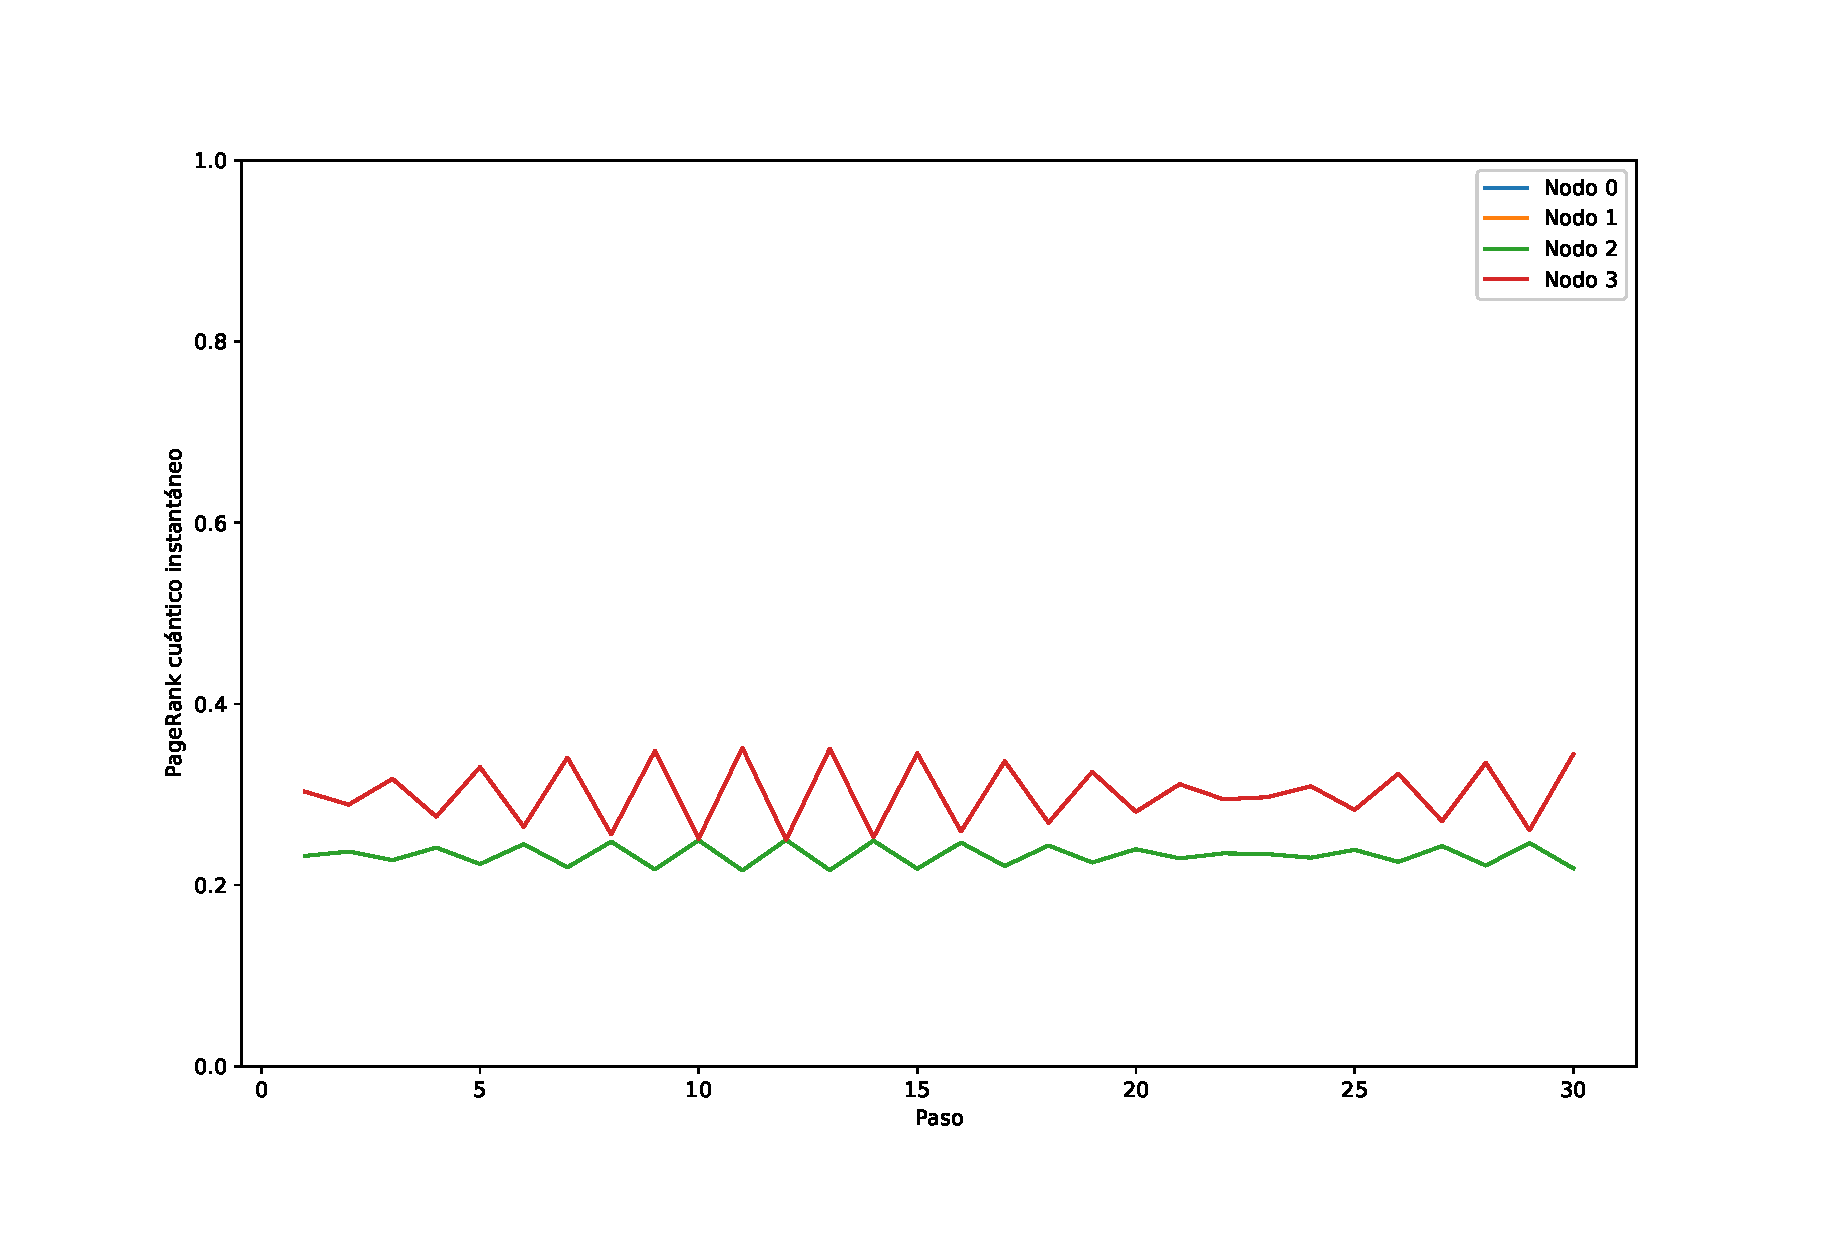
\includegraphics[width=0.9\linewidth]{img/crown-inst-M.eps}
        \caption{Wolfram Mathematica}
    \end{subfigure}
    \begin{subfigure}[m]{0.45\textwidth}
        \centering
        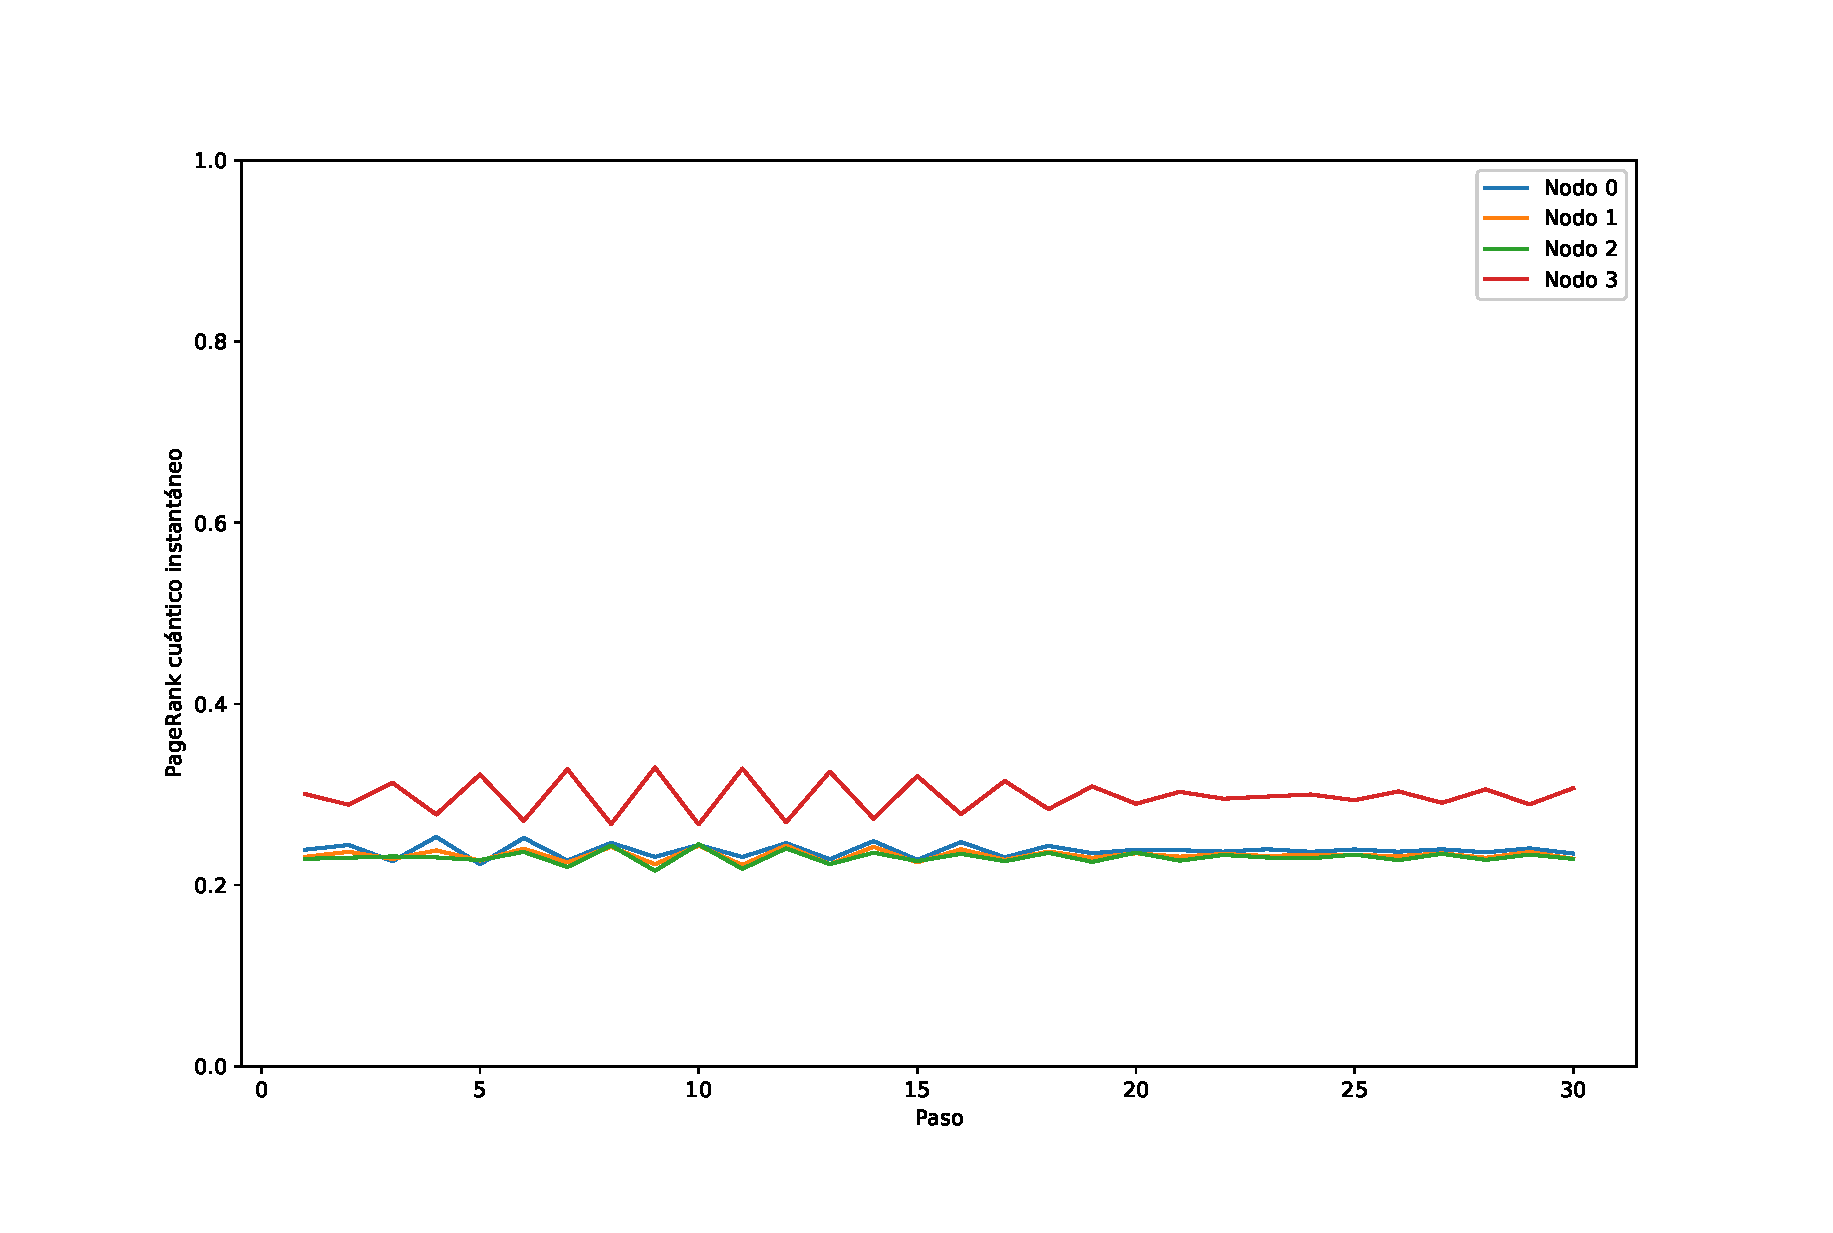
\includegraphics[width=0.9\linewidth]{img/crown-inst-lossless.eps}
        \caption{Python}
    \end{subfigure}
    \caption[PageRank cuántico instantáneo del grafo corona sin pérdidas]{PageRank cuántico instantáneo del grafo corona sin pérdidas}
    \label{fig:instcrownlossless}
\end{figure}

\begin{figure}[H]
    \centering
    \begin{subfigure}[m]{0.45\textwidth}
        \centering
        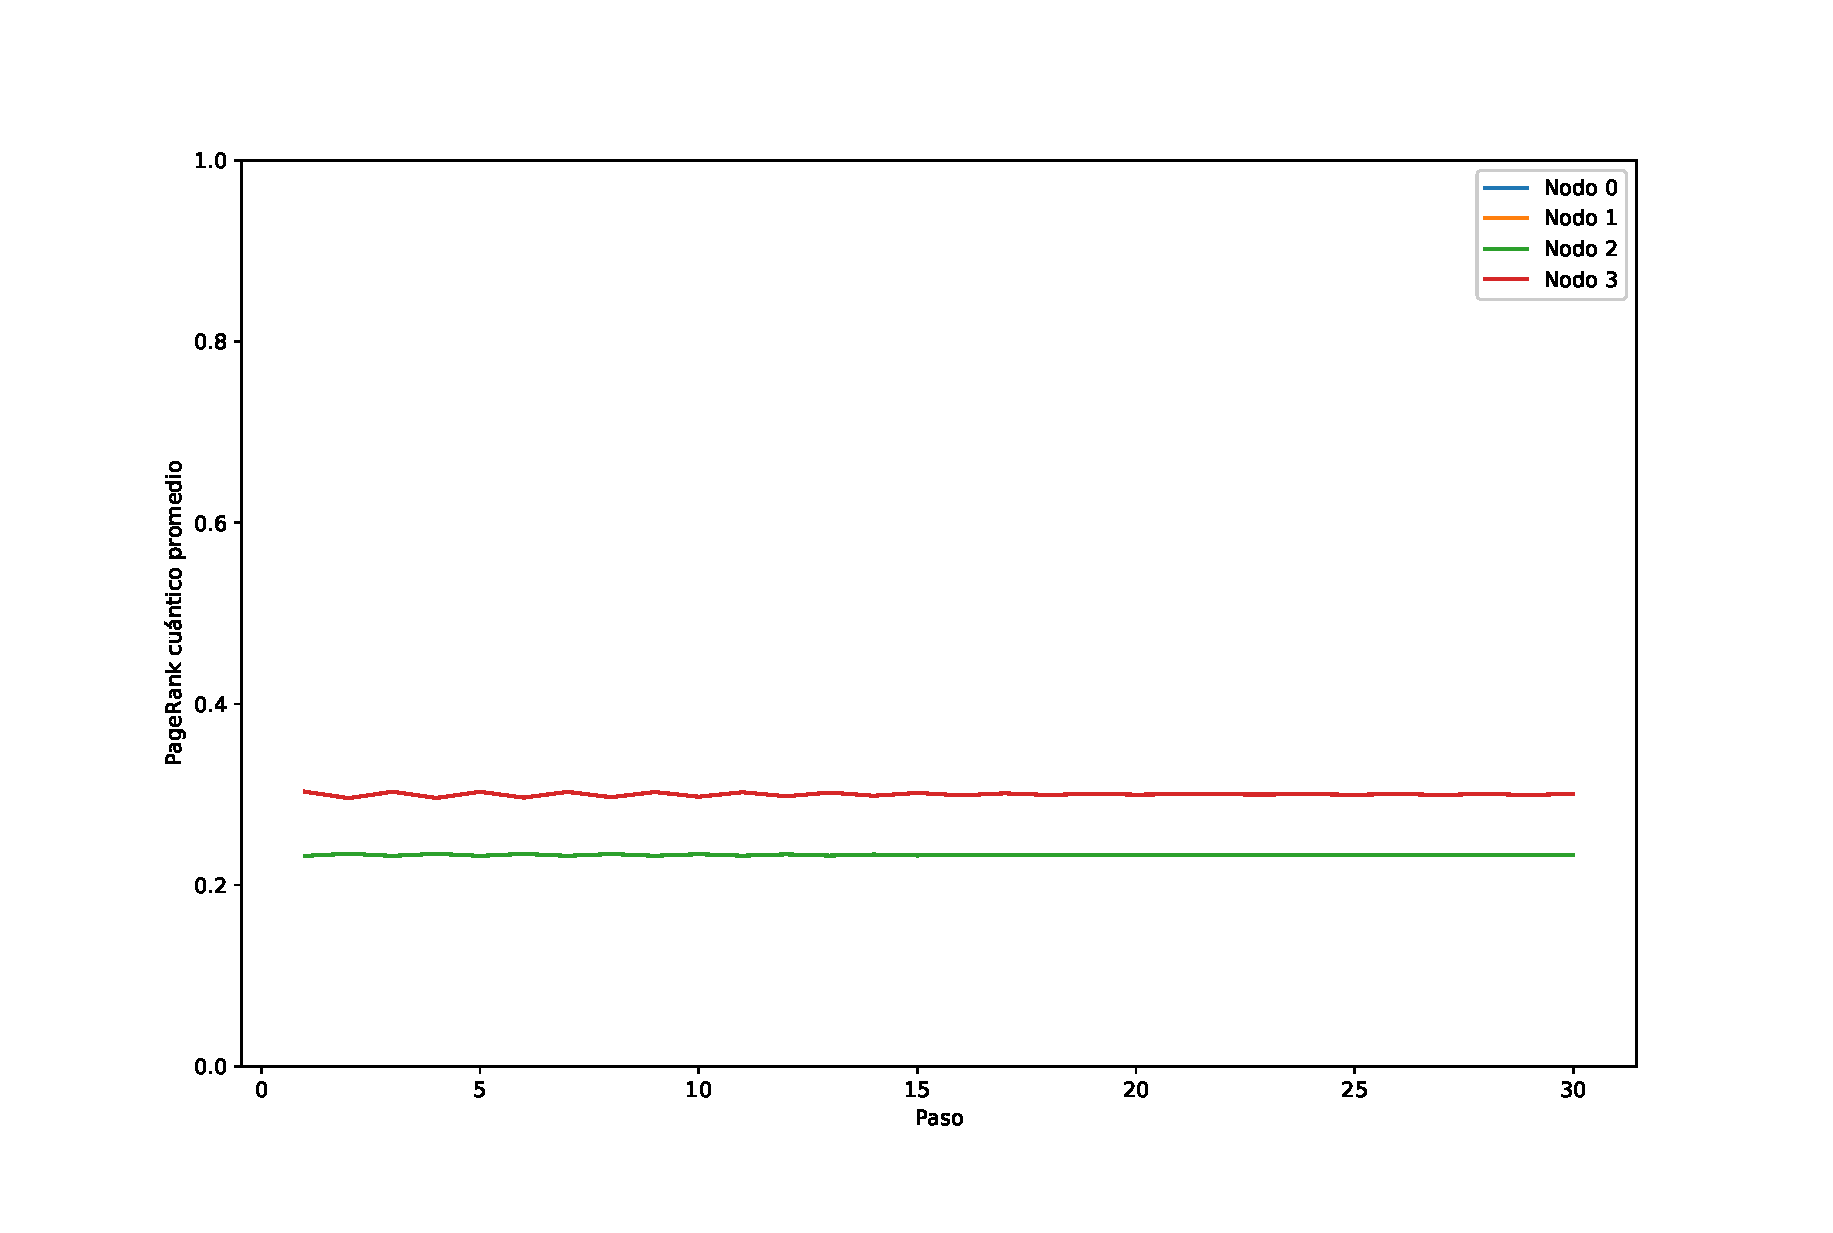
\includegraphics[width=0.9\linewidth]{img/crown-mean-M.eps}
        \caption{Wolfram Mathematica}
    \end{subfigure}
    \begin{subfigure}[m]{0.45\textwidth}
        \centering
        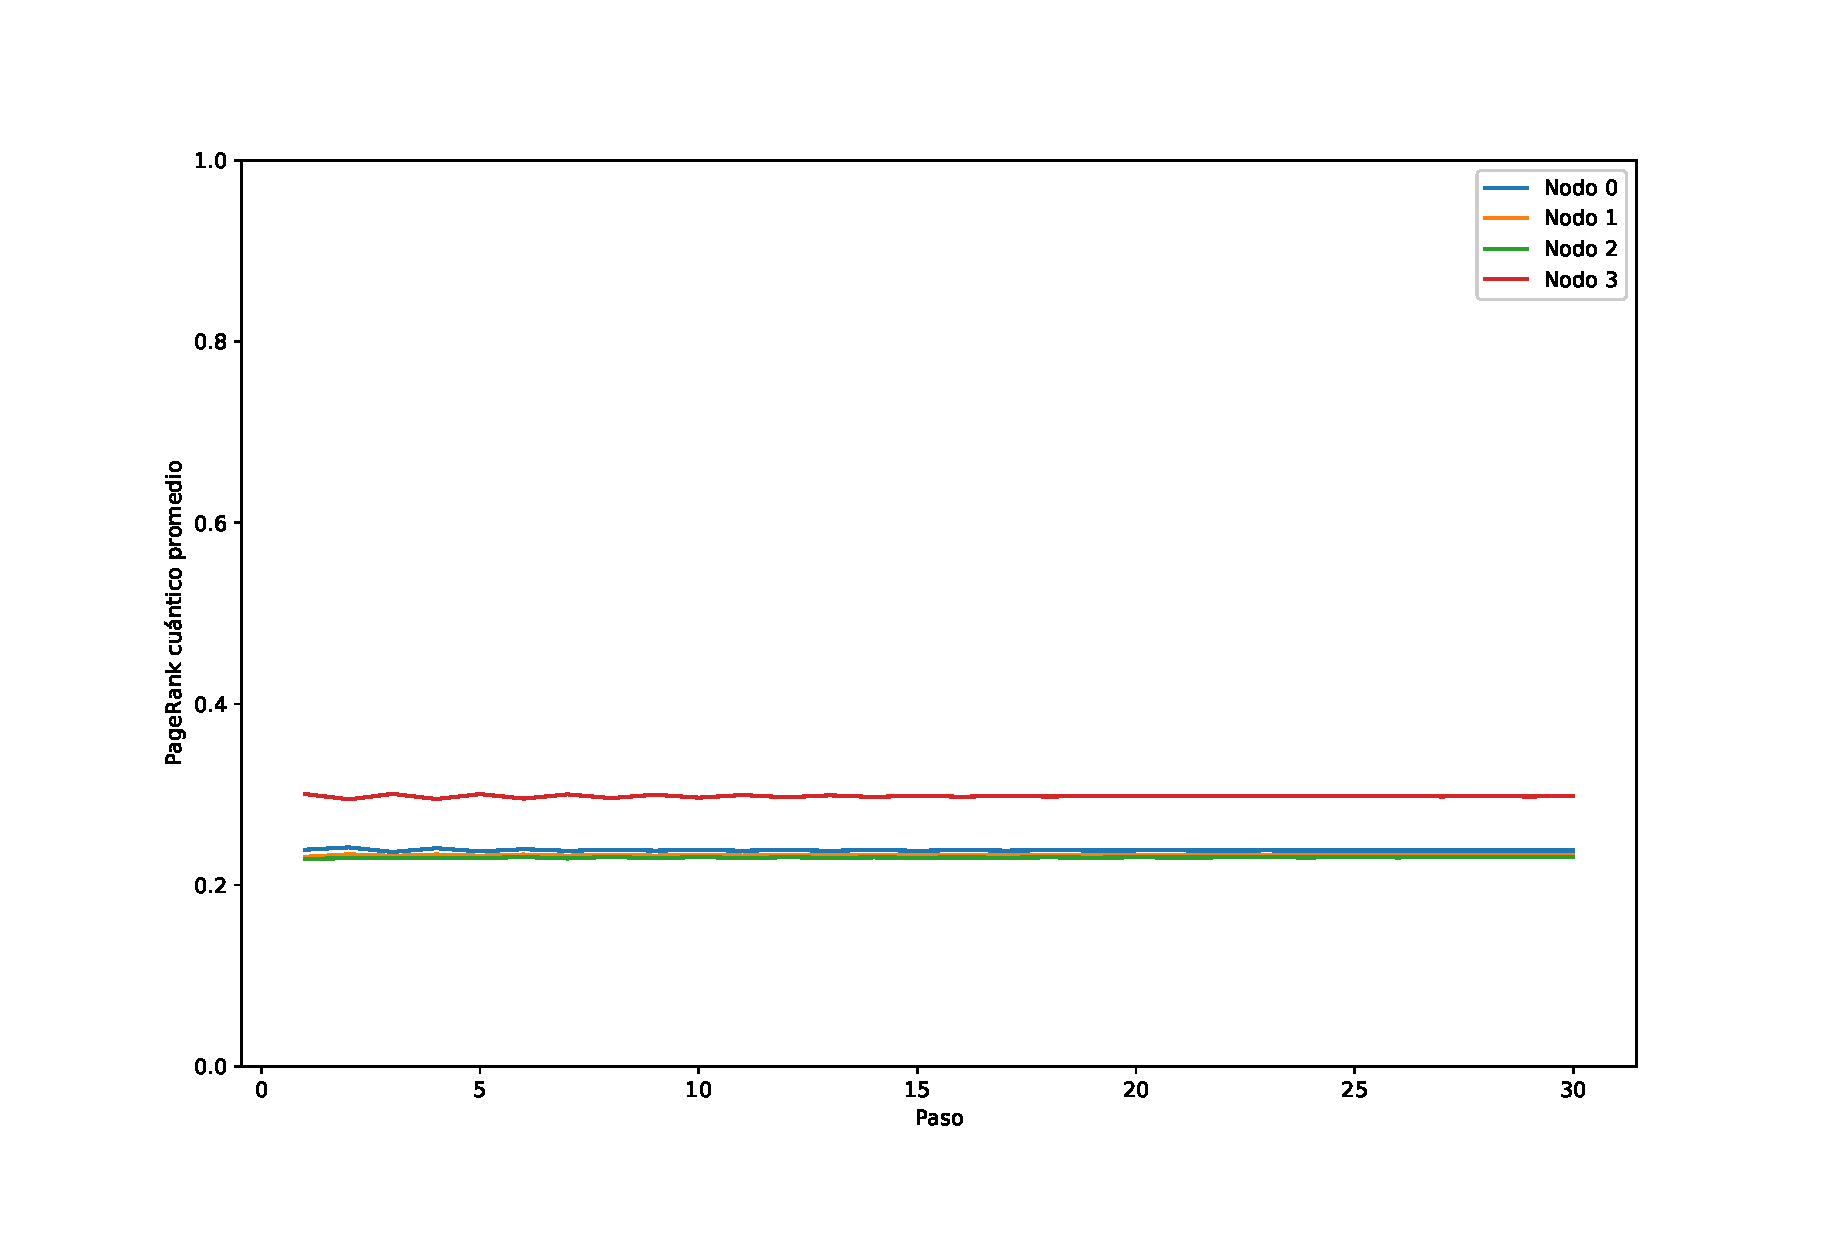
\includegraphics[width=0.9\linewidth]{img/crown-mean-lossless.eps}
        \caption{Python}
    \end{subfigure}
    \caption[PageRank cuántico promedio del grafo corona sin pérdidas]{PageRank cuántico promedio del grafo corona sin pérdidas}
    \label{fig:meancrownlossless}
\end{figure}

\begin{figure}[H]
    \centering
    \begin{subfigure}[m]{0.45\textwidth}
        \centering
        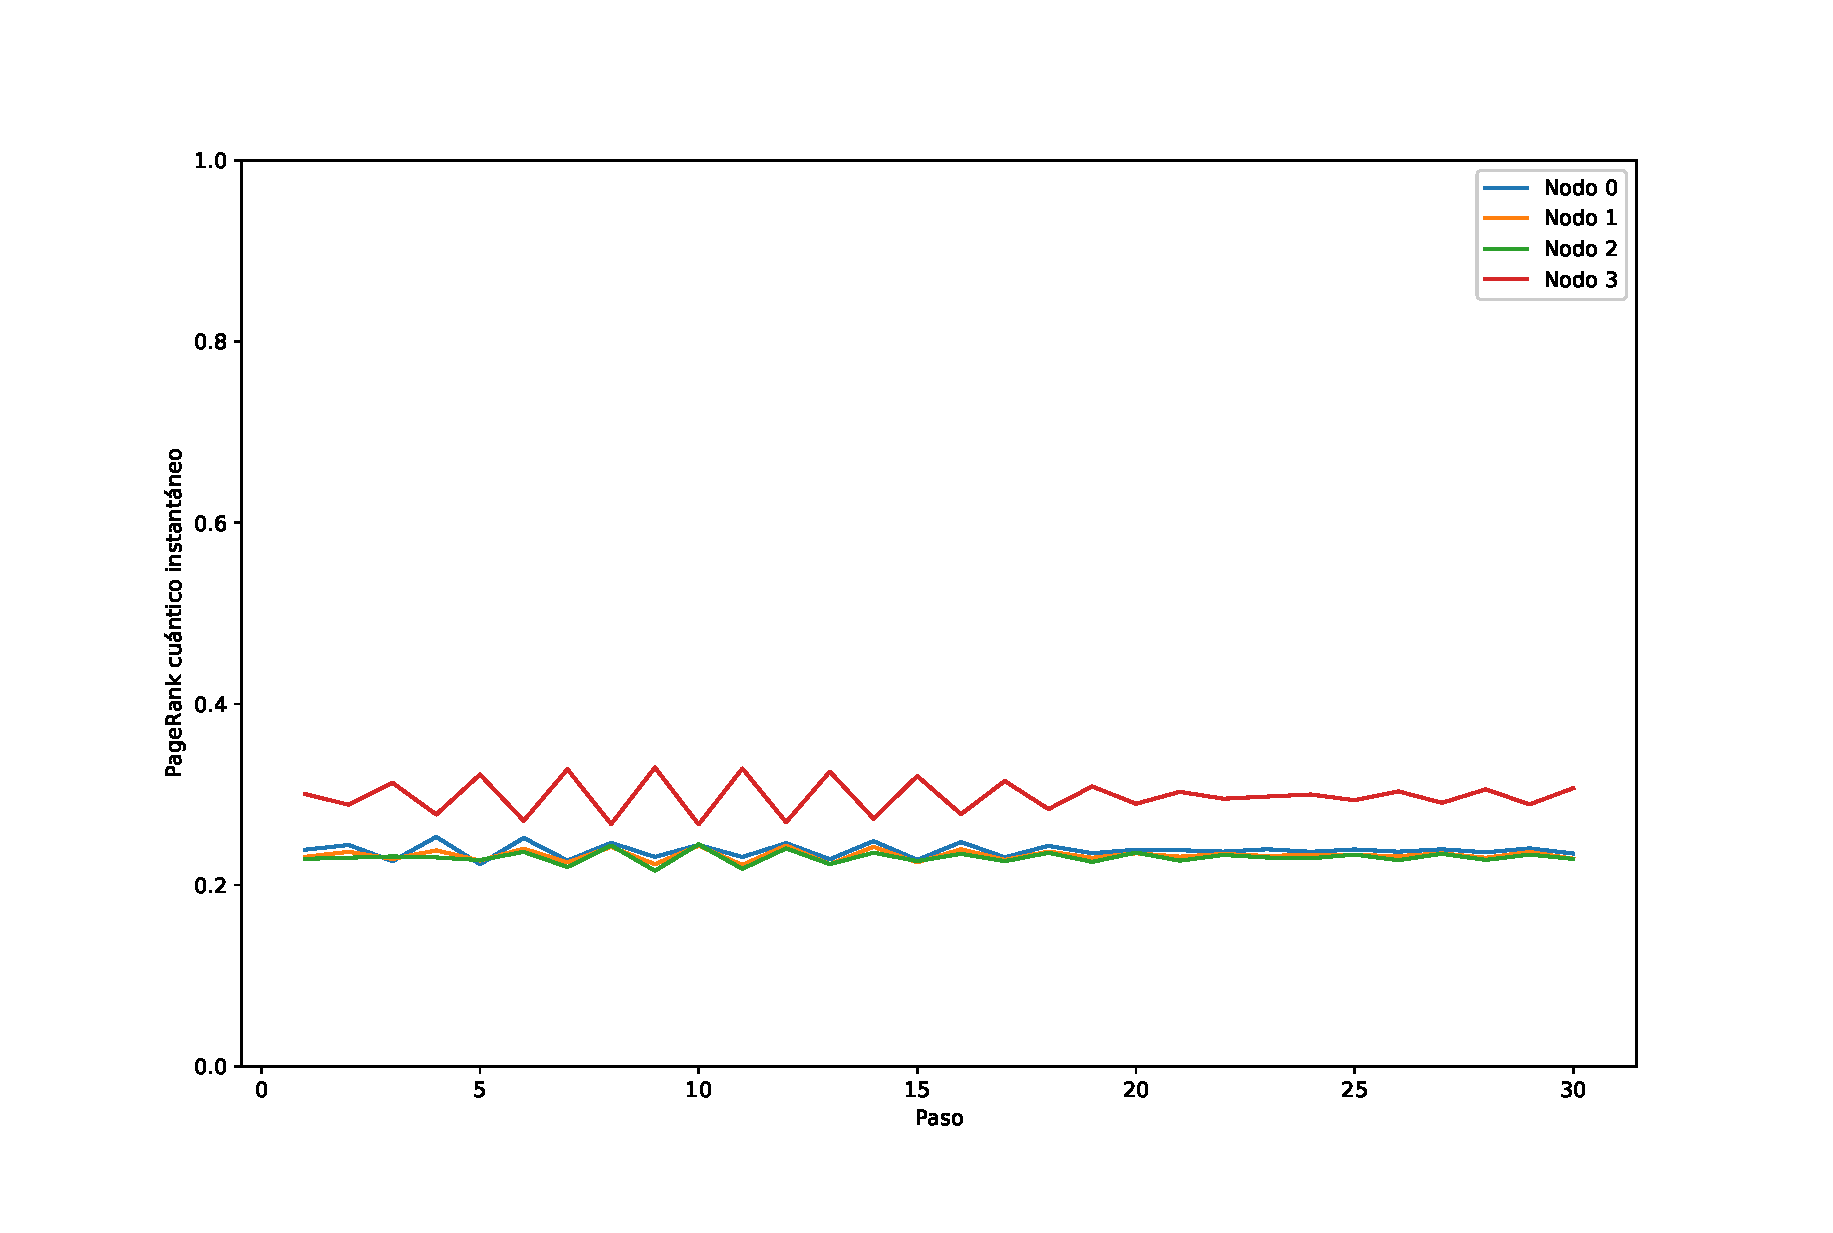
\includegraphics[width=0.9\linewidth]{img/crown-inst-lossless.eps}
        \caption{Sin relajación}
    \end{subfigure}
    \begin{subfigure}[m]{0.45\textwidth}
        \centering
        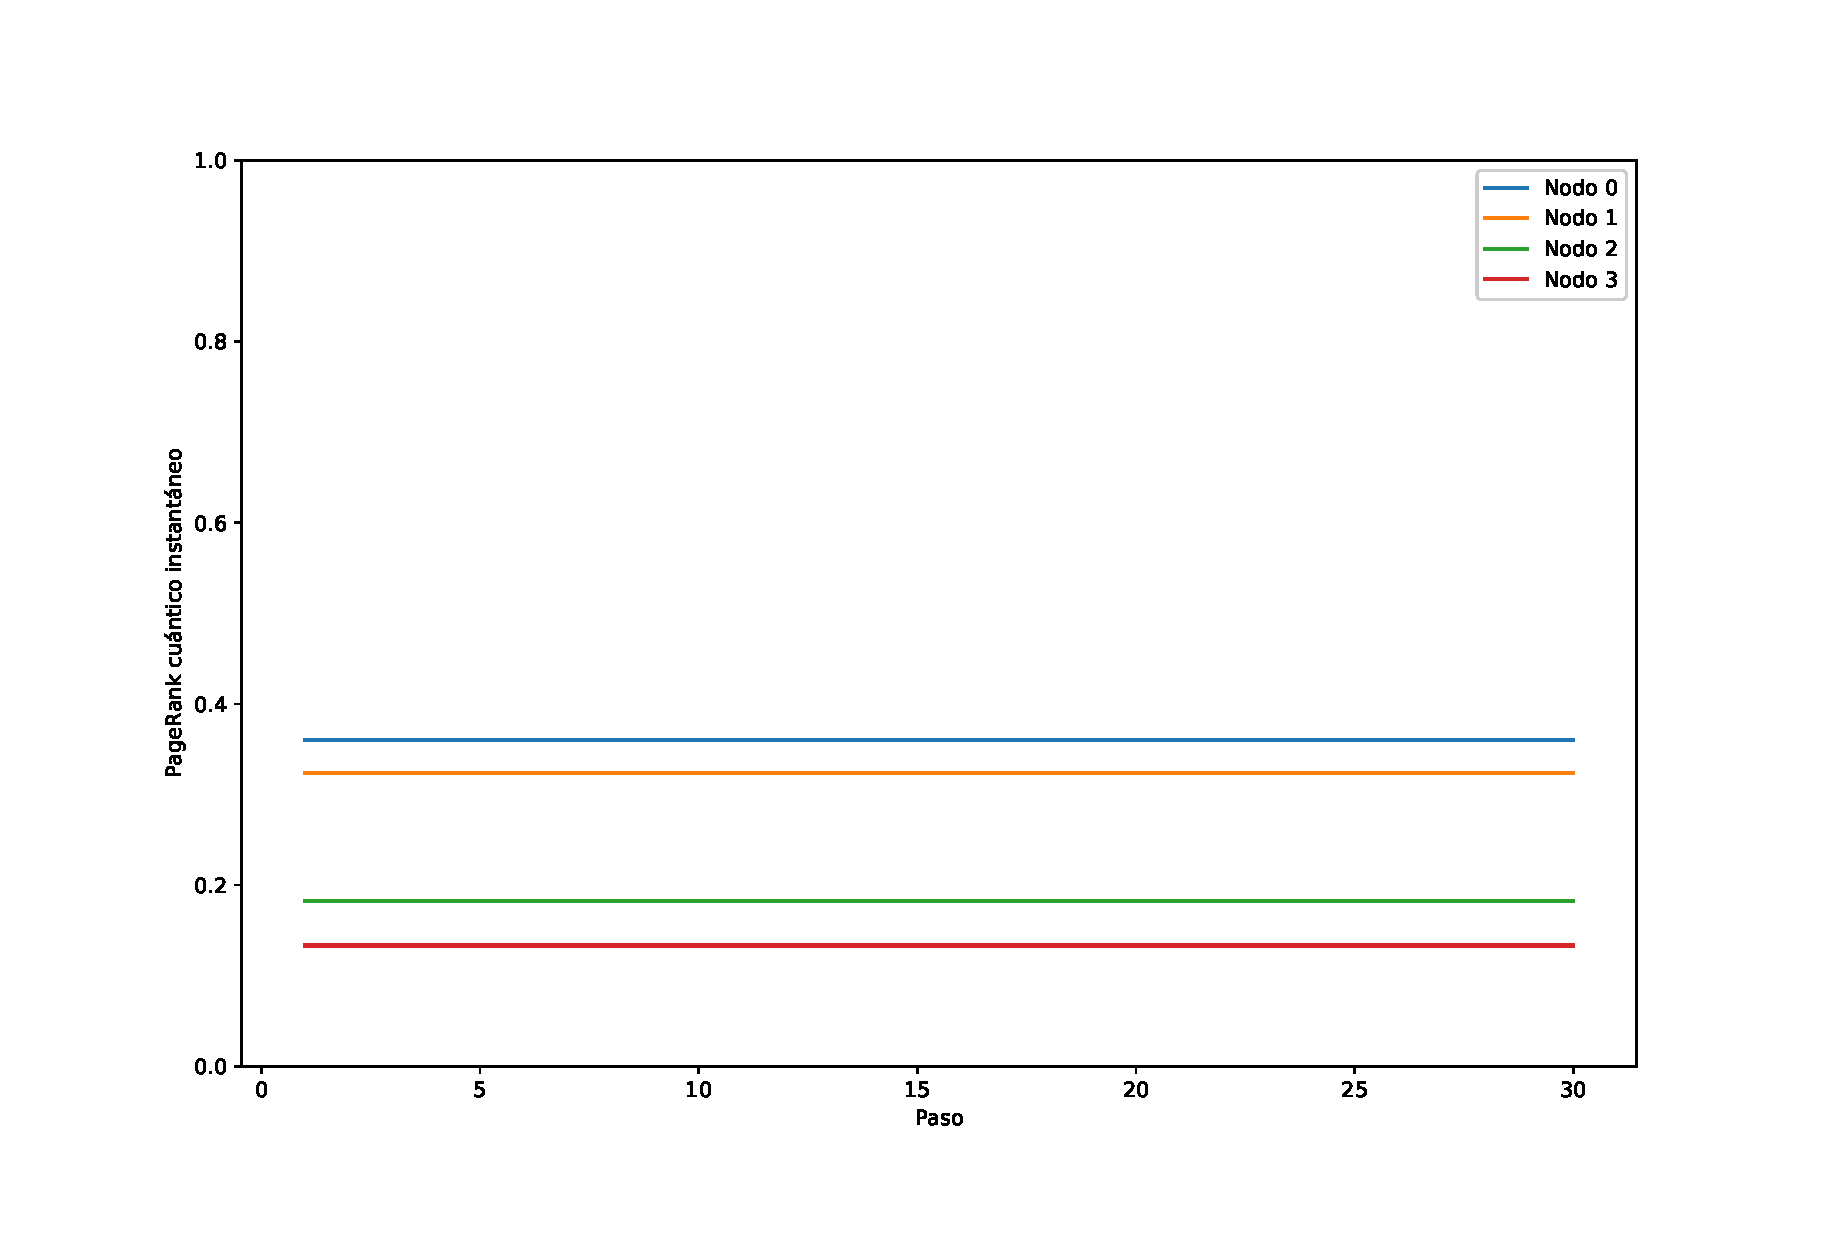
\includegraphics[width=0.9\linewidth]{img/crown-inst-lossy.eps}
        \caption{Con relajación}
    \end{subfigure}
    \caption[PageRank cuántico instantaneo del grafo aleatorio con y sin pérdidas]{PageRank cuántico instantaneo del grafo aleatorio con y sin pérdidas}
    \label{fig:instcrownlossy}
\end{figure}

\begin{figure}[H]
    \centering
    \begin{subfigure}[m]{0.45\textwidth}
        \centering
        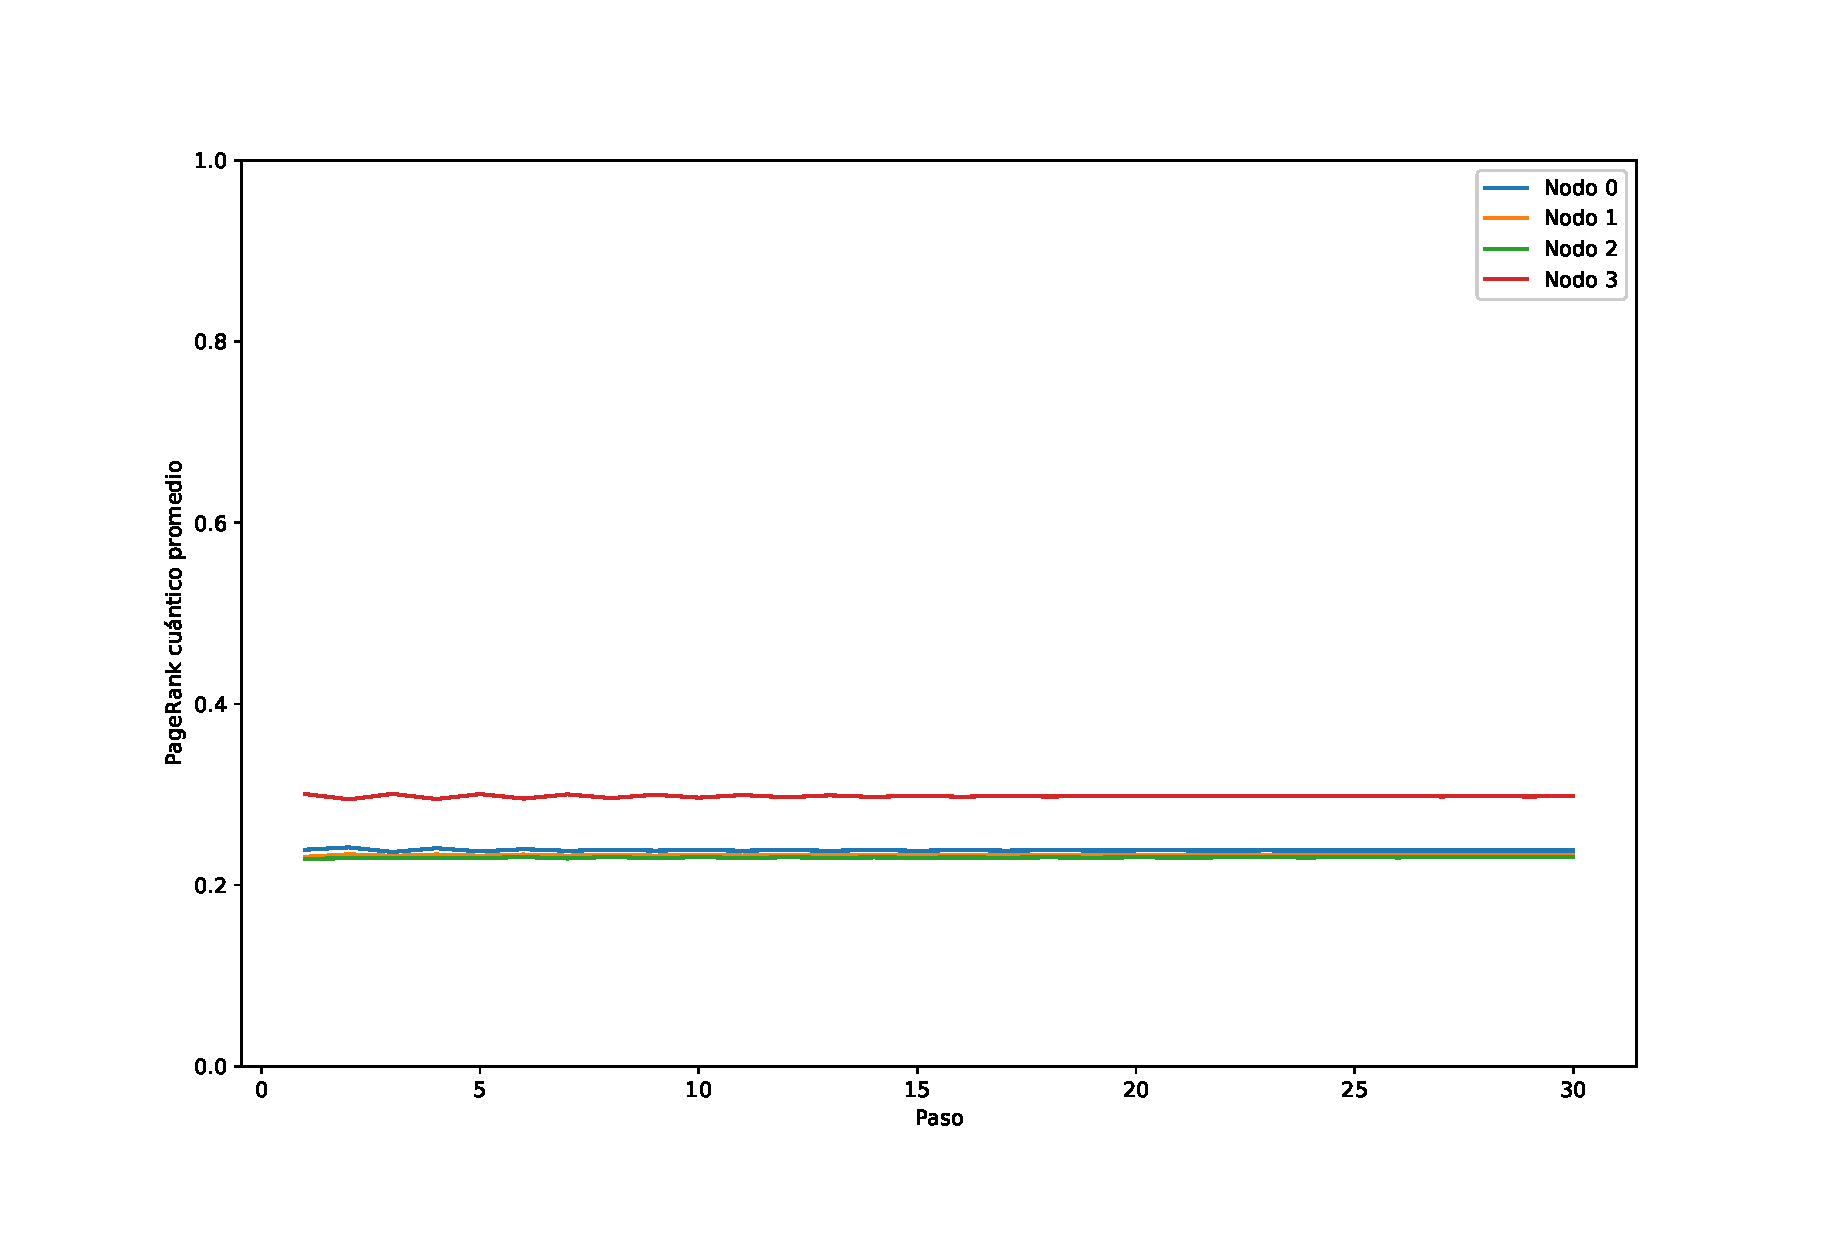
\includegraphics[width=0.9\linewidth]{img/crown-mean-lossless.eps}
        \caption{Sin relajación}
    \end{subfigure}
    \begin{subfigure}[m]{0.45\textwidth}
        \centering
        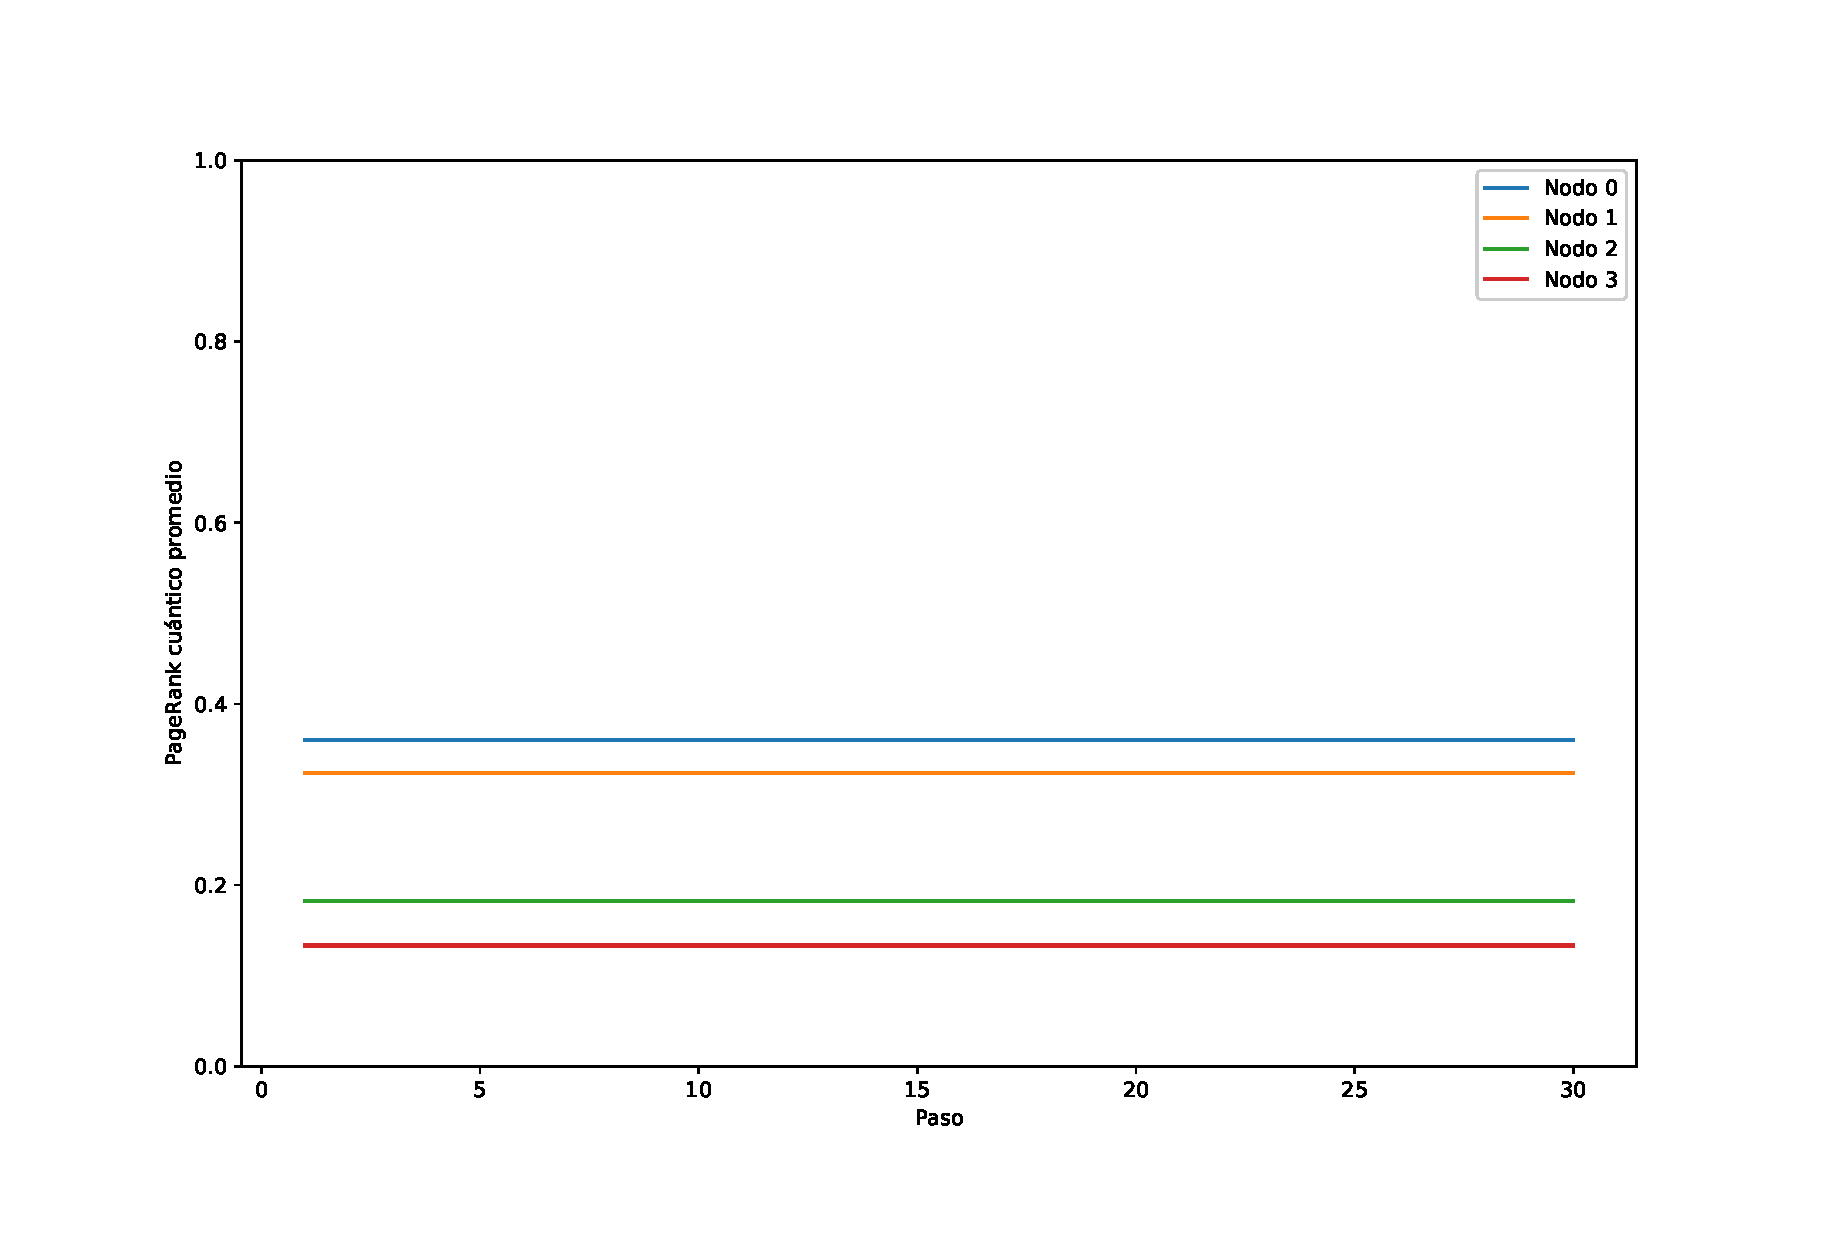
\includegraphics[width=0.9\linewidth]{img/crown-mean-lossy.eps}
        \caption{Con relajación}
    \end{subfigure}
    \caption[PageRank cuántico promedio del grafo aleatorio con y sin pérdidas]{PageRank cuántico promedio del grafo aleatorio con y sin pérdidas}
    \label{fig:meancrownlossy}
\end{figure}










\begin{figure}[H]
    \centering
    \begin{tikzpicture}[->,>=stealth',shorten >=1pt,thick]
    \SetGraphUnit{2} 
    \tikzset{VertexStyle/.style = {draw,circle,thick,
                                   minimum size=0.5cm,
                                   font=\bfseries},thick} 
    \Vertex{1} \SOWE(1){2} \SOEA(1){3} \SO(2){4} 
    \Edge(1)(2)
    \Edge(1)(3)
    \Edge(2)(4)
    \end{tikzpicture} 
    \caption[Grafo árbol]{Grafo árbol}
    \label{fig:tree}
\end{figure}

\begin{equation}
    A = 
    \begin{pmatrix}
        0 & 0 & 0 & 0 \\
        1 & 0 & 0 & 0 \\
        1 & 0 & 0 & 0 \\
        0 & 1 & 0 & 0 \\
    \end{pmatrix}
\end{equation}

\begin{equation}
    E =
    \begin{pmatrix}
        0 & 0 & \frac{1}{4} & \frac{1}{4} \\
        \frac{1}{2} & 0 & \frac{1}{4} & \frac{1}{4} \\
        \frac{1}{2} & 0 & \frac{1}{4} & \frac{1}{4} \\
        0 & 1 & \frac{1}{4} & \frac{1}{4} \\
    \end{pmatrix}
\end{equation}

\begin{equation}
    G =
    \begin{pmatrix}
        \frac{3}{80} & \frac{3}{80} & \frac{1}{4} & \frac{1}{4} \\
        \frac{37}{80} & \frac{3}{80} & \frac{1}{4} & \frac{1}{4} \\
        \frac{37}{80} & \frac{3}{80} & \frac{1}{4} & \frac{1}{4} \\
        \frac{3}{80} & \frac{71}{80} & \frac{1}{4} & \frac{1}{4} \\
    \end{pmatrix}
\end{equation}

\begin{figure}[H]
\[\Qcircuit @C=1.4em @R=1.8em {
& \gate{Ry(1.5708)} & \ctrlo{1}           & \ctrl{1}          & \qw \\
& \qw                & \gate{Ry(2.58678)}  & \gate{Ry(0.554811)} & \qw \\
} \]
\caption{Circuito de $K_1$ para el grafo árbol}
\label{fig:treekb1}
\end{figure}

\begin{figure}[H]
\[\Qcircuit @C=1.4em @R=1.8em {
& \gate{Ry(2.58678)} & \ctrlo{1}           & \ctrl{1}          & \qw \\
& \qw                & \gate{Ry(1.5708)}  & \gate{Ry(2.73613)} & \qw \\
} \]
\caption{Circuito de $K_2$ para el grafo árbol}
\label{fig:treekb2}
\end{figure}

\begin{figure}[H]
\[\Qcircuit @C=1.4em @R=1.8em {
& \gate{Ry(\pi/2)}    & \qw               & \qw \\
& \qw                 & \gate{Ry(\pi/2)}  & \qw \\
} \]
\caption{Circuito de $K_3$ para el grafo árbol}
\label{fig:treekb3}
\end{figure}

\begin{figure}[H]
\[\Qcircuit @C=1.4em @R=1.8em {
& \ctrlo{1}          & \ctrlo{1}          & \ctrl{2}           & \qw \\
& \ctrlo{1}          & \ctrl{1}           & \qw                & \qw \\
& \multigate{1}{K_1} & \multigate{1}{K_2} & \multigate{1}{K_3} & \qw \\
& \ghost{K_1}        & \ghost{K_2}        & \ghost{K_3}        & \qw \\
} 
\]
\caption[$K_b$ del grafo árbol]{$K_b$ del grafo árbol}
\label{fig:treekb}
\end{figure}

\begin{figure}[H]
\[\Qcircuit @C=1.4em @R=1.8em {
& \gate{I} & \qw \\
& \gate{I} & \qw \\
& \gate{I} & \qw \\
& \gate{I} & \qw \\
} 
\]
\caption[$T$ del grafo árbol]{$T$ del grafo árbol}
\label{fig:treeT}
\end{figure}

\begin{figure}[H]
\[\Qcircuit @C=1.4em @R=1.8em {
& \gate{H} & \multigate{3}{K_b} & \qw \\
& \gate{H} & \ghost{K_b}        & \qw \\
& \qw      & \ghost{K_b}        & \qw \\
& \qw      & \ghost{K_b}        & \qw \\
} 
\]
\caption{Preparación del estado inicial para la caminata en el grafo árbol}
\label{fig:treeinit}
\end{figure}

\begin{figure}[H]
\[ \Qcircuit @C=1.4em @R=1.8em {
\lstick{\ket{0}} & {/^4} \qw & \gate{Init} & \gate{K_b^\dagger} & \gate{D} & \gate{K_b} & \gate{SWAP} & \meter & \cw \\
& & & & \rstick{ 2m \text{ veces}}
\gategroup{1}{4}{1}{7}{1.3em}{_\}}
} \]
\caption{Circuito del PageRank cuántico  del grafo árbol}
\label{fig:loketree}
\end{figure}

\begin{figure}[H]
    \centering
    \begin{subfigure}[m]{0.45\textwidth}
        \centering
        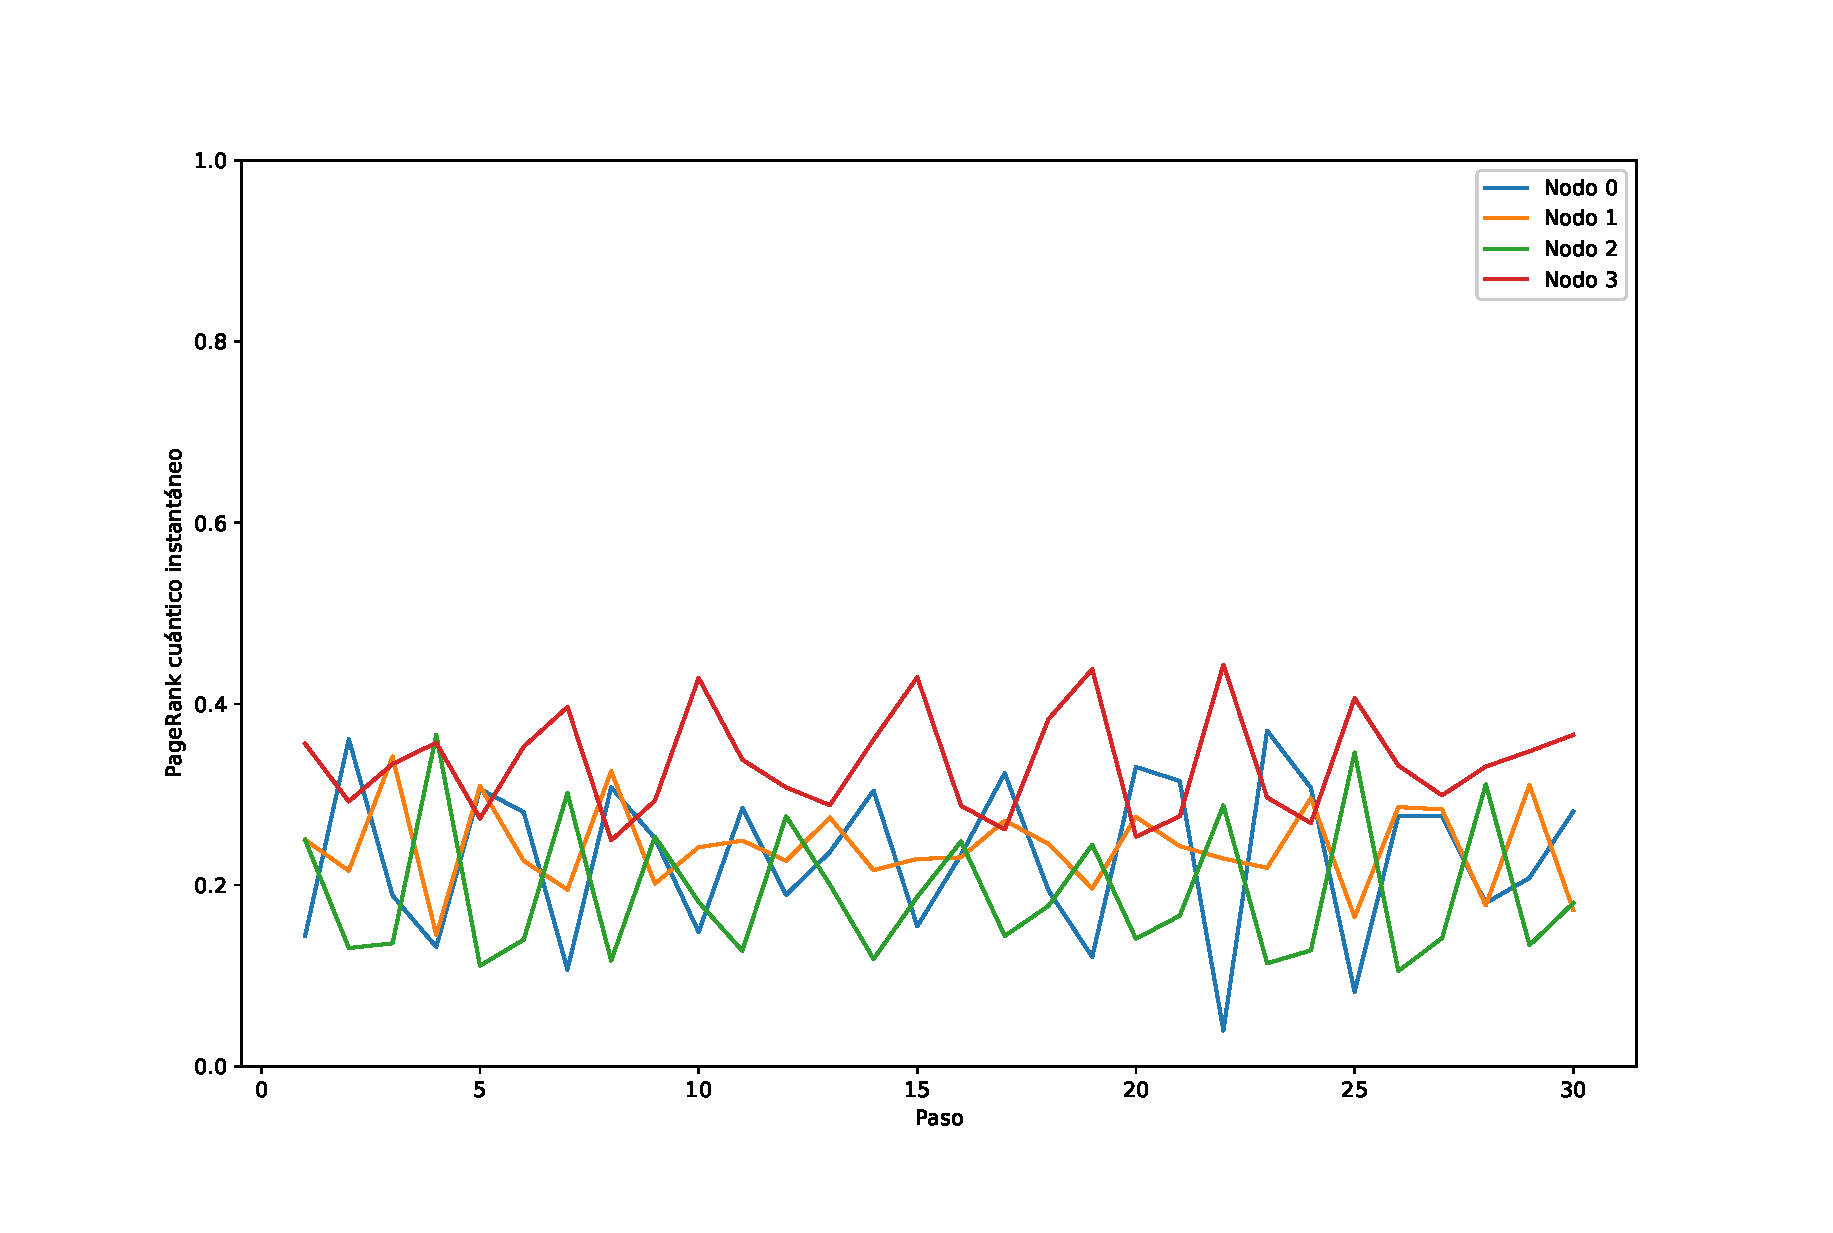
\includegraphics[width=0.9\linewidth]{img/tree-inst-M.eps}
        \caption{Wolfram Mathematica}
    \end{subfigure}
    \begin{subfigure}[m]{0.45\textwidth}
        \centering
        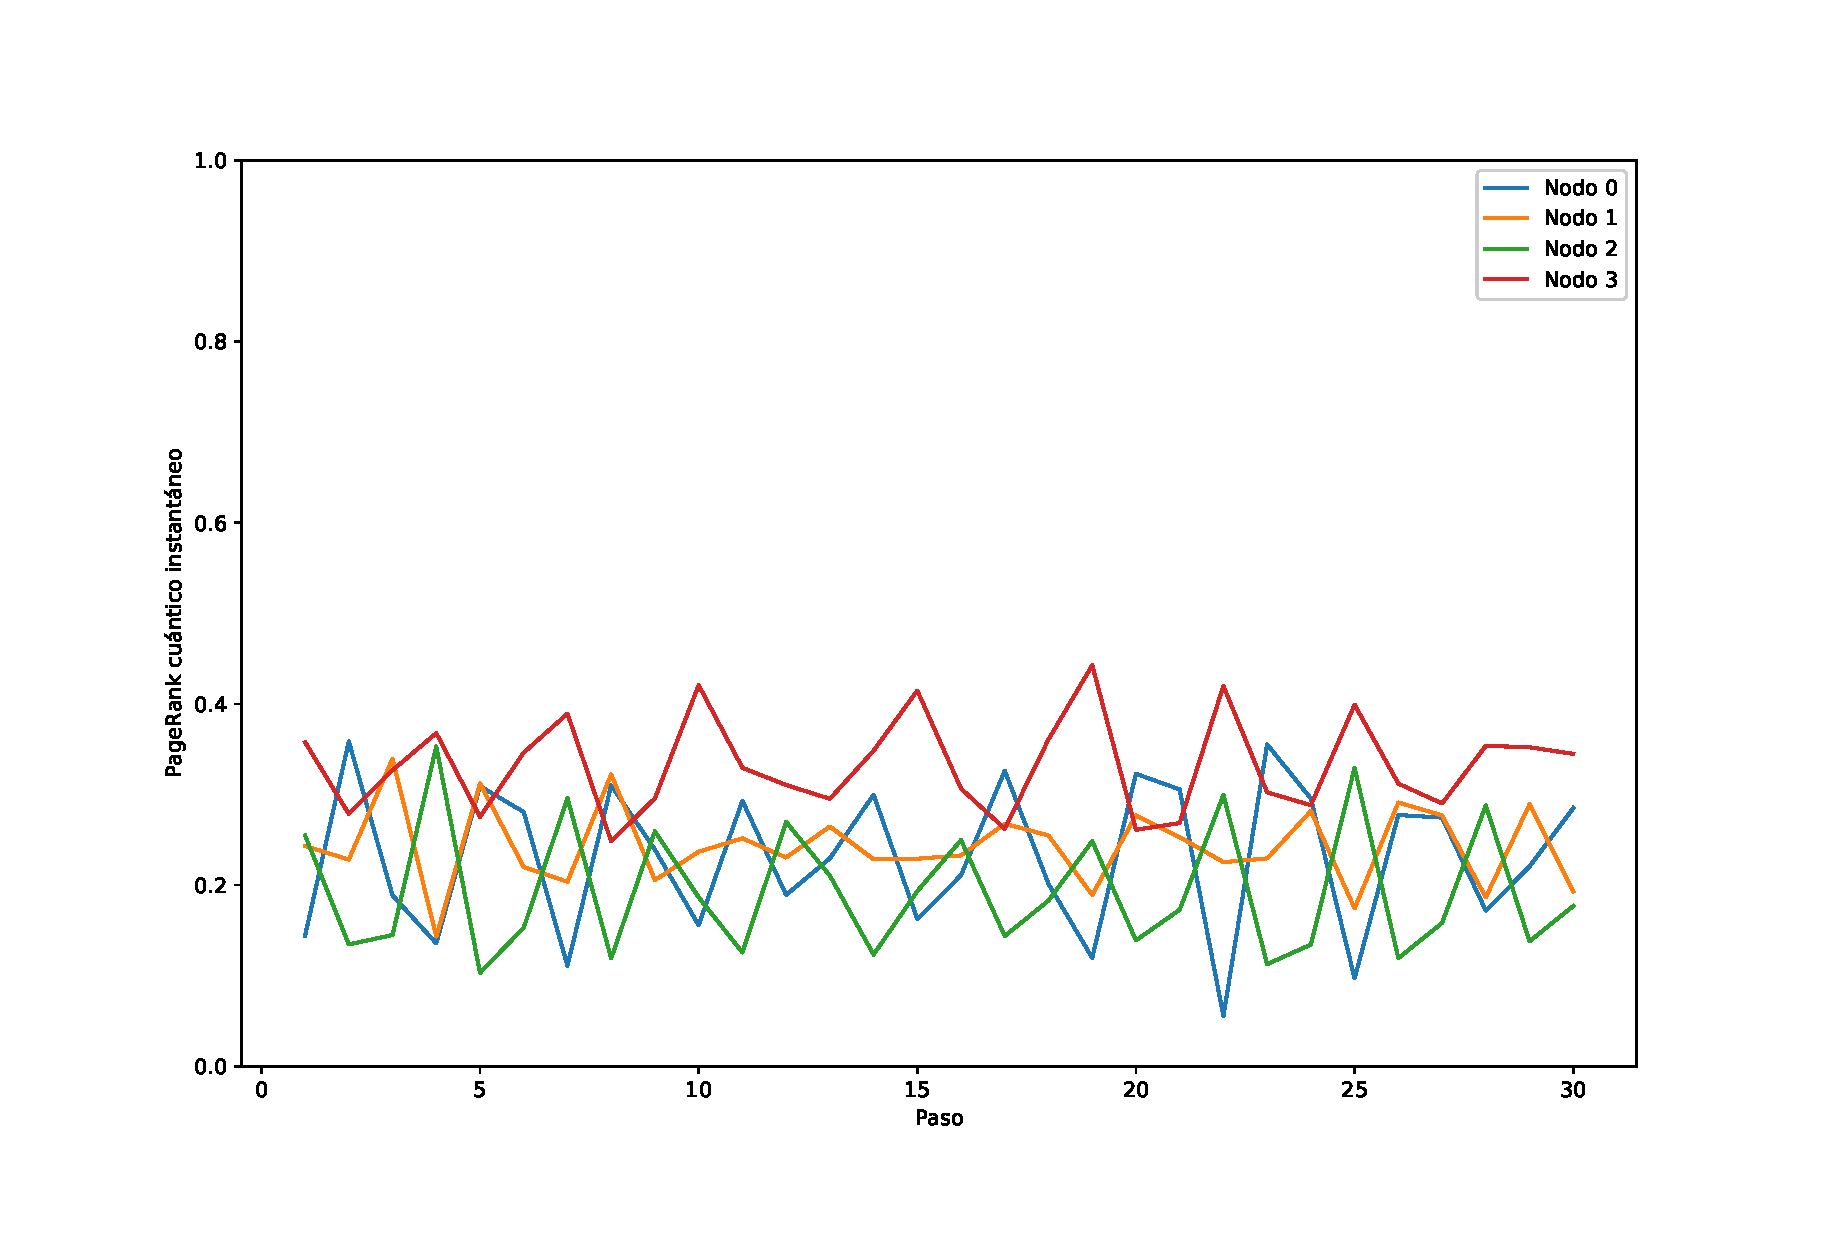
\includegraphics[width=0.9\linewidth]{img/tree-inst-lossless.eps}
        \caption{Python}
    \end{subfigure}
    \caption[PageRank cuántico instantáneo del grafo árbol sin pérdidas]{PageRank cuántico instantáneo del grafo árbol sin pérdidas}
    \label{fig:insttreelossless}
\end{figure}

\begin{figure}[H]
    \centering
    \begin{subfigure}[m]{0.45\textwidth}
        \centering
        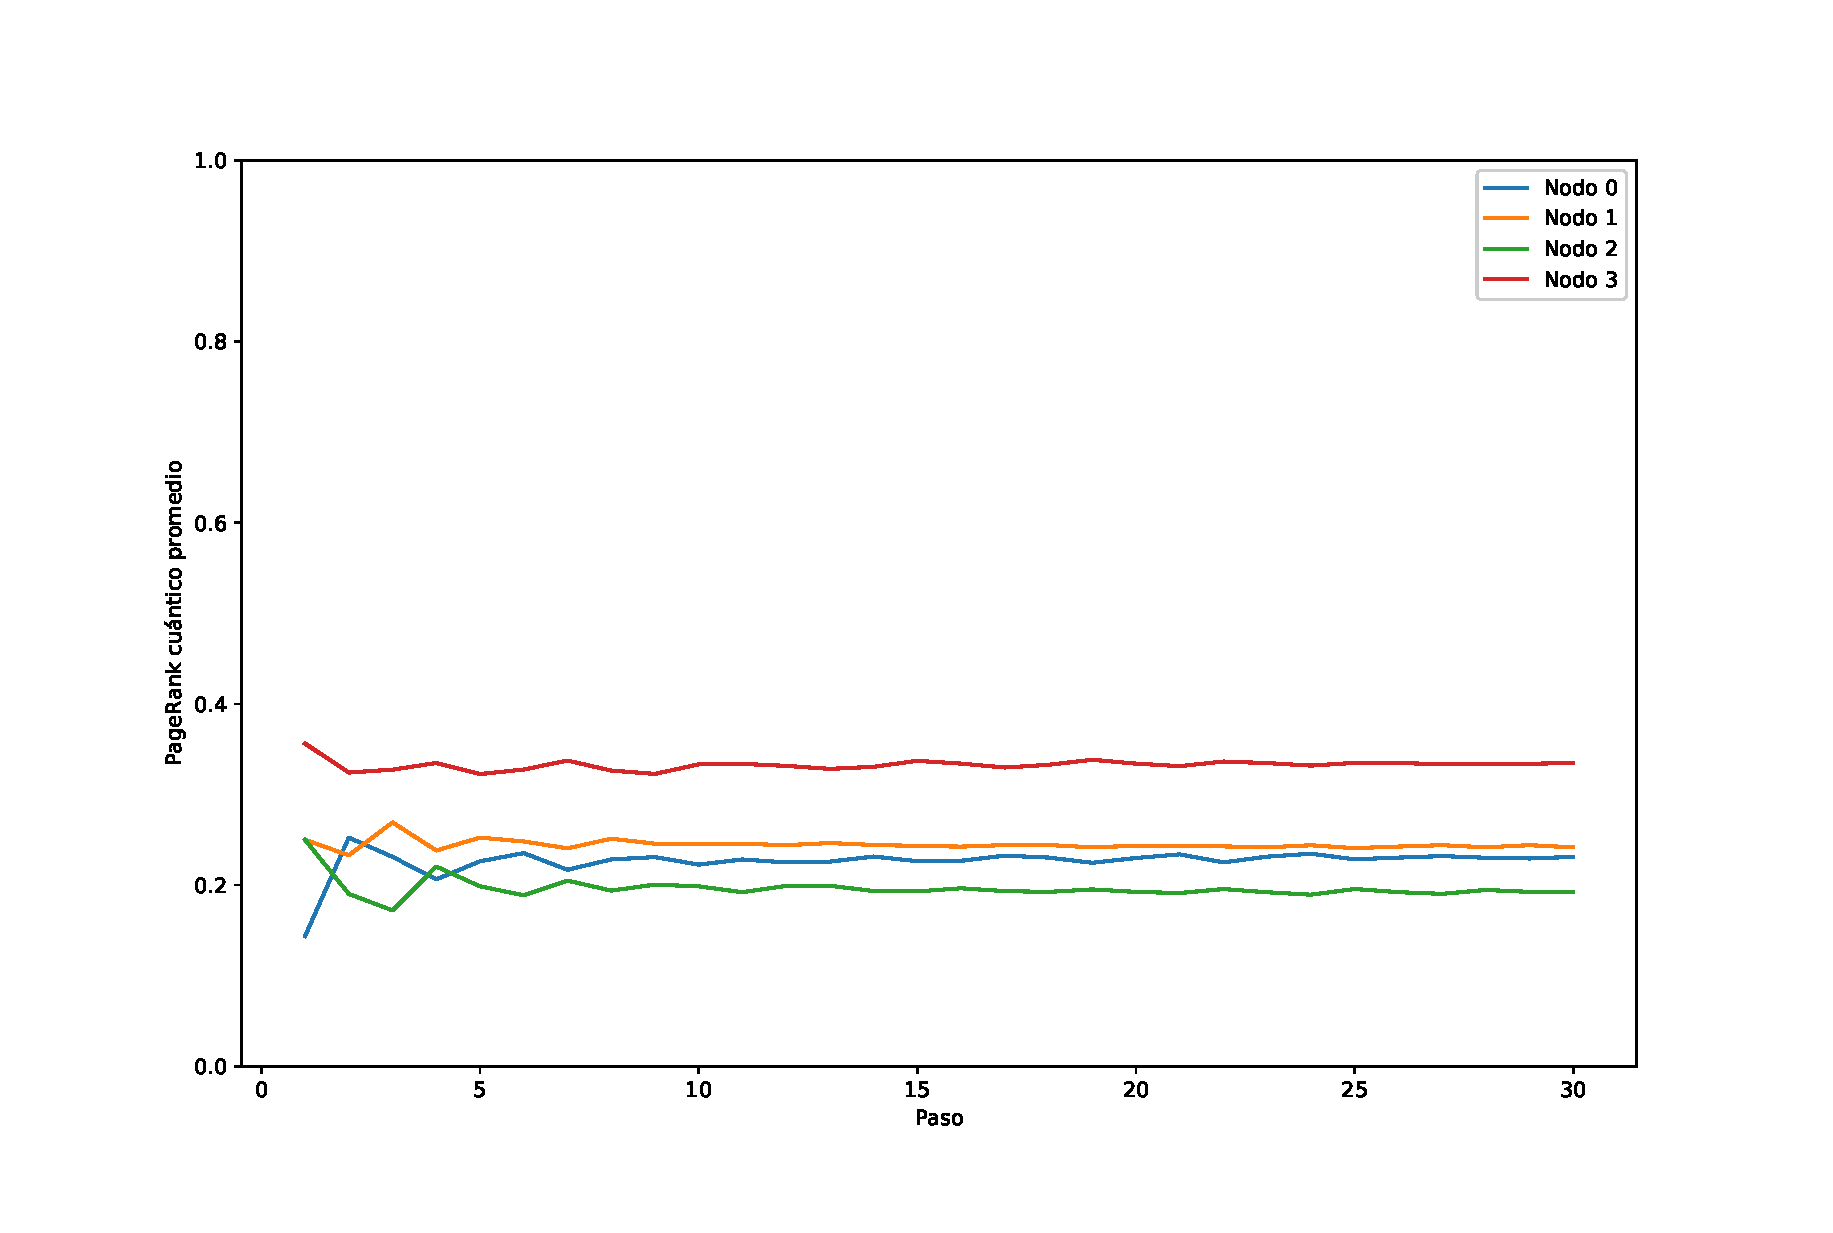
\includegraphics[width=0.9\linewidth]{img/tree-mean-M.eps}
        \caption{Wolfram Mathematica}
    \end{subfigure}
    \begin{subfigure}[m]{0.45\textwidth}
        \centering
        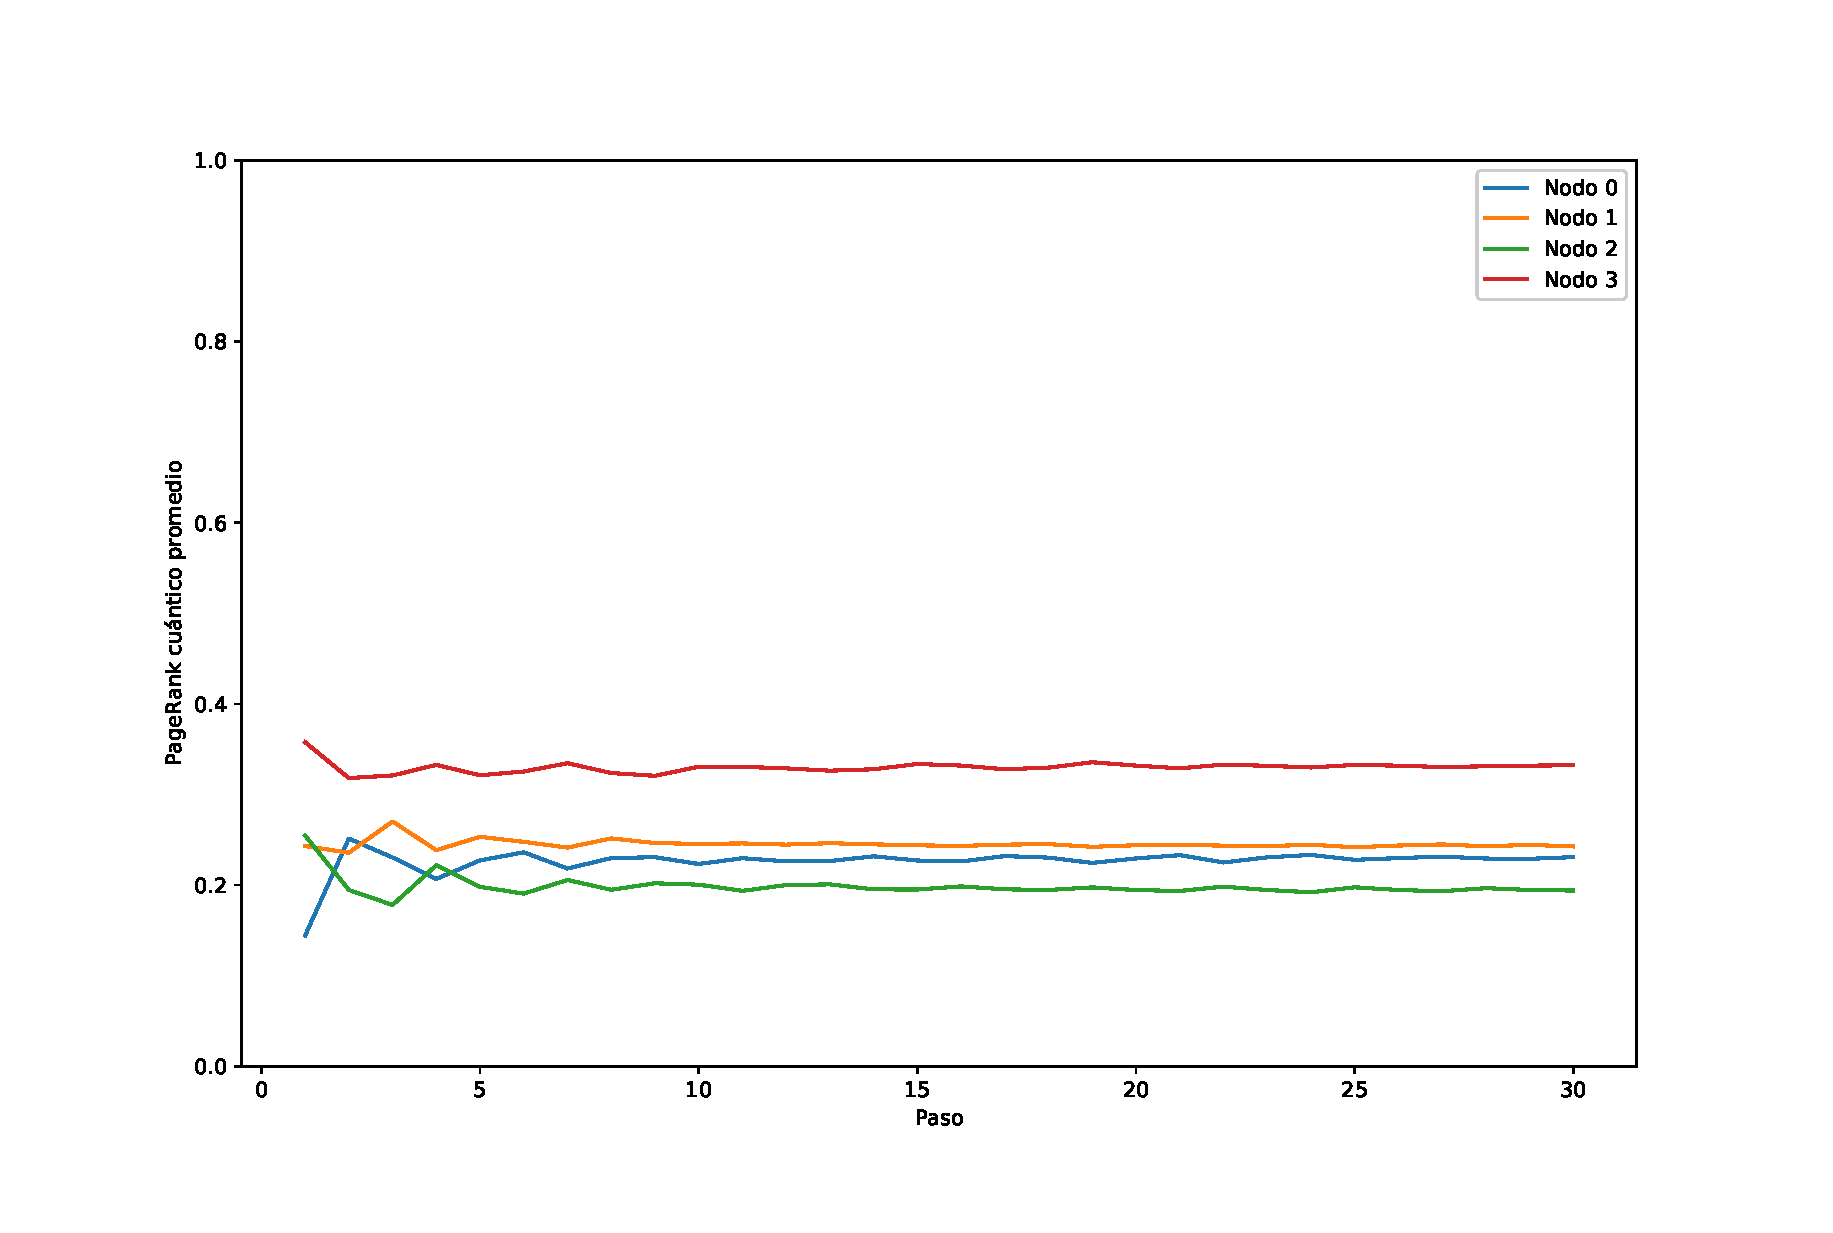
\includegraphics[width=0.9\linewidth]{img/tree-mean-lossless.eps}
        \caption{Python}
    \end{subfigure}
    \caption[PageRank cuántico promedio del grafo árbol sin pérdidas]{PageRank cuántico promedio del grafo árbol sin pérdidas}
    \label{fig:meantreelossless}
\end{figure}

\begin{figure}[H]
    \centering
    \begin{subfigure}[m]{0.45\textwidth}
        \centering
        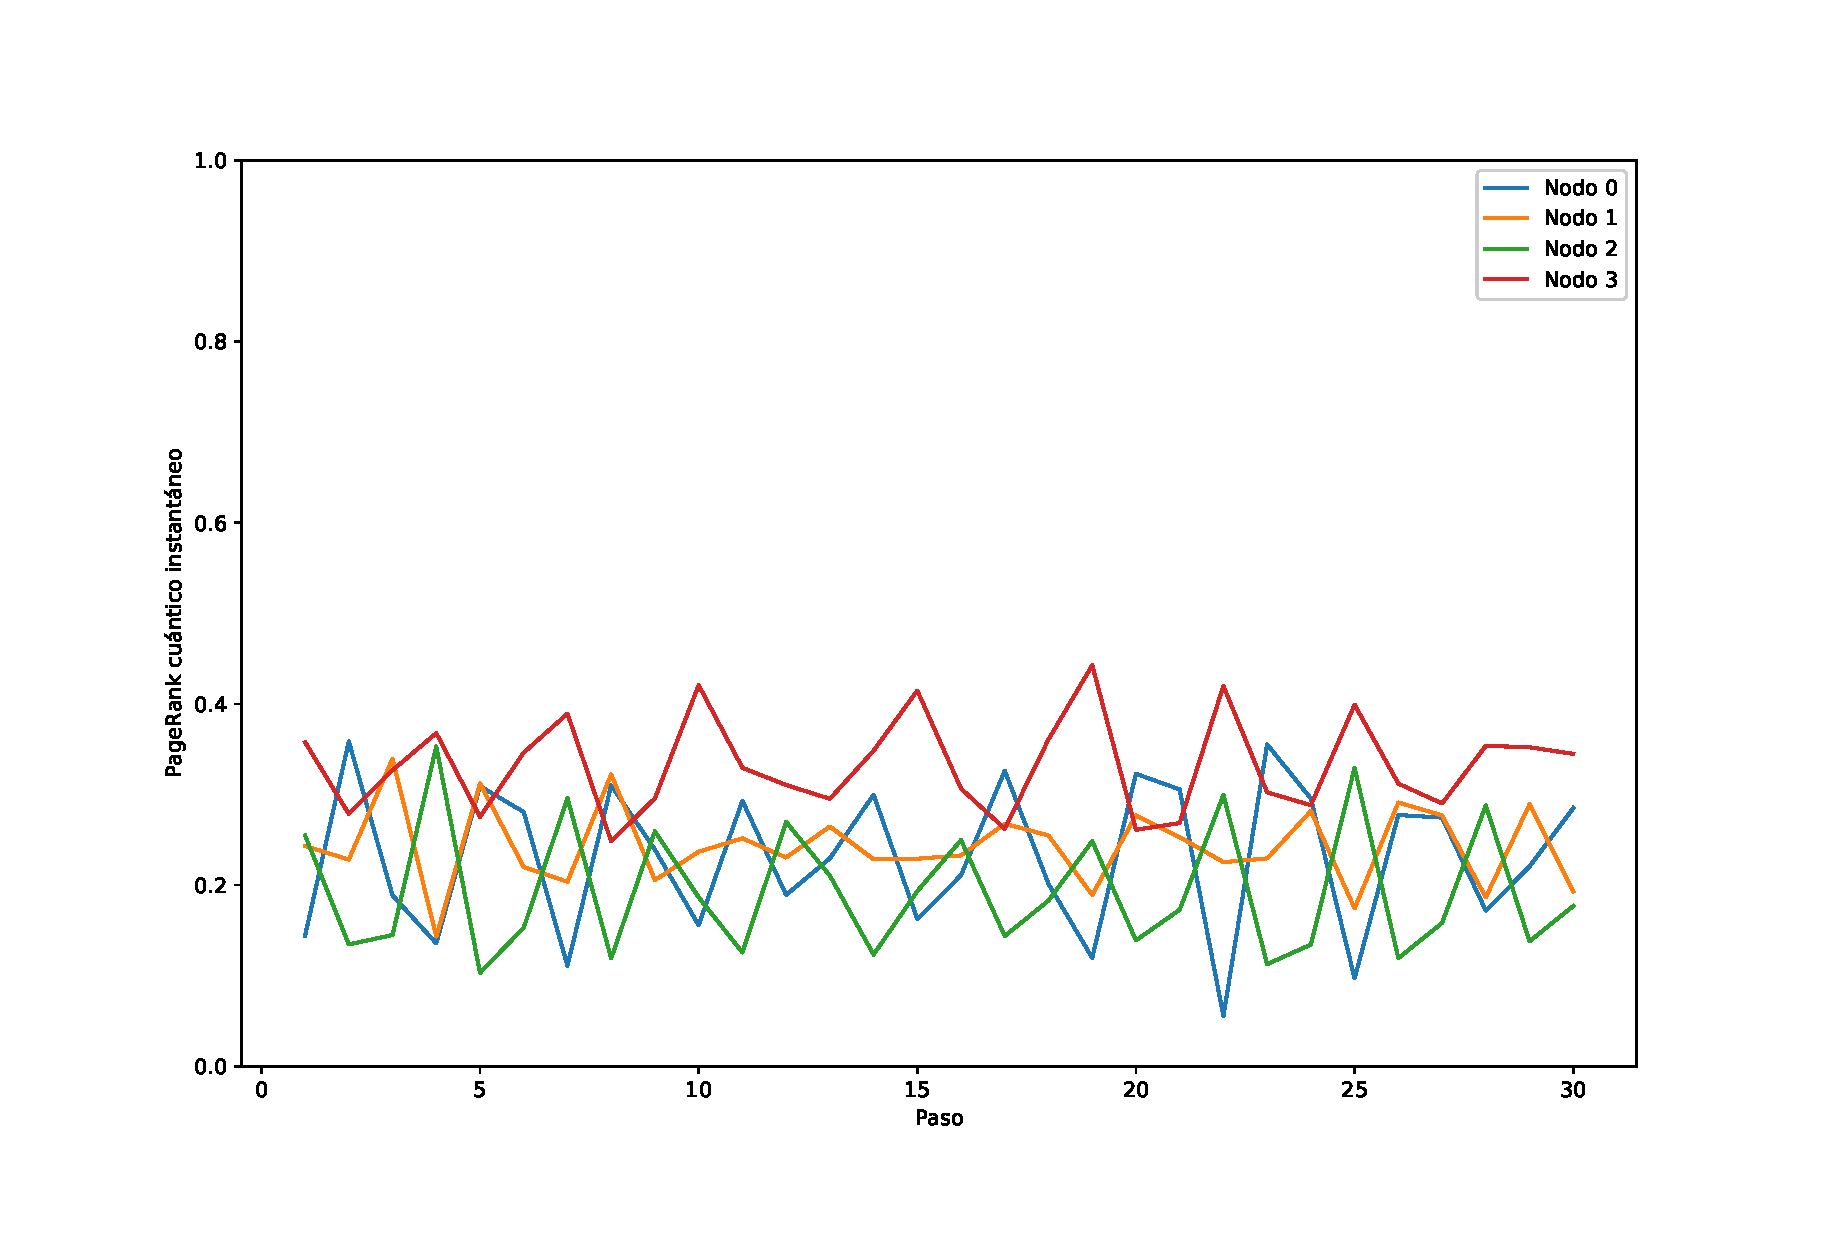
\includegraphics[width=0.9\linewidth]{img/tree-inst-lossless.eps}
        \caption{Sin relajación}
    \end{subfigure}
    \begin{subfigure}[m]{0.45\textwidth}
        \centering
        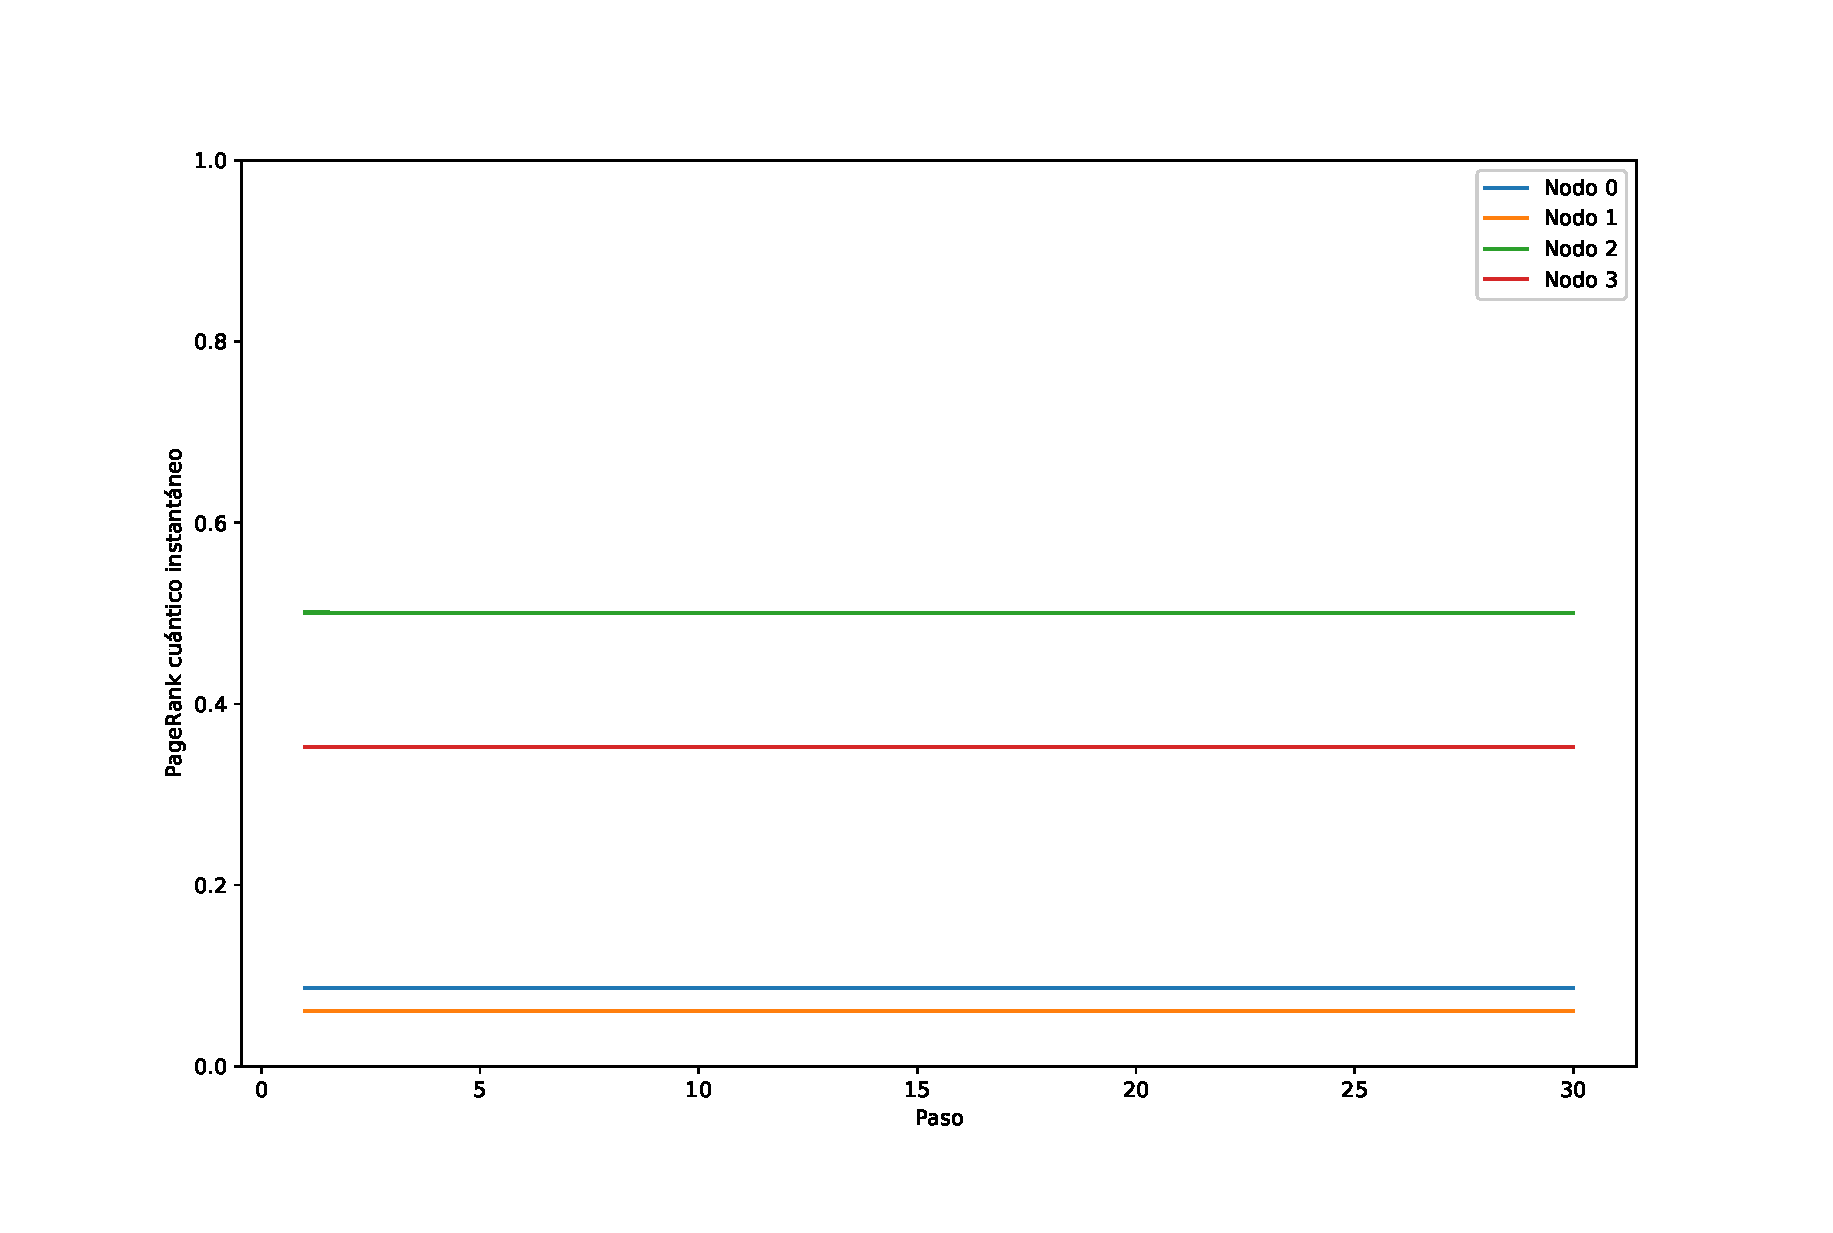
\includegraphics[width=0.9\linewidth]{img/tree-inst-lossy.eps}
        \caption{Con relajación}
    \end{subfigure}
    \caption[PageRank cuántico instantaneo del grafo árbol con y sin pérdidas]{PageRank cuántico instantaneo del grafo árbol con y sin pérdidas}
    \label{fig:insttreelossy}
\end{figure}

\begin{figure}[H]
    \centering
    \begin{subfigure}[m]{0.45\textwidth}
        \centering
        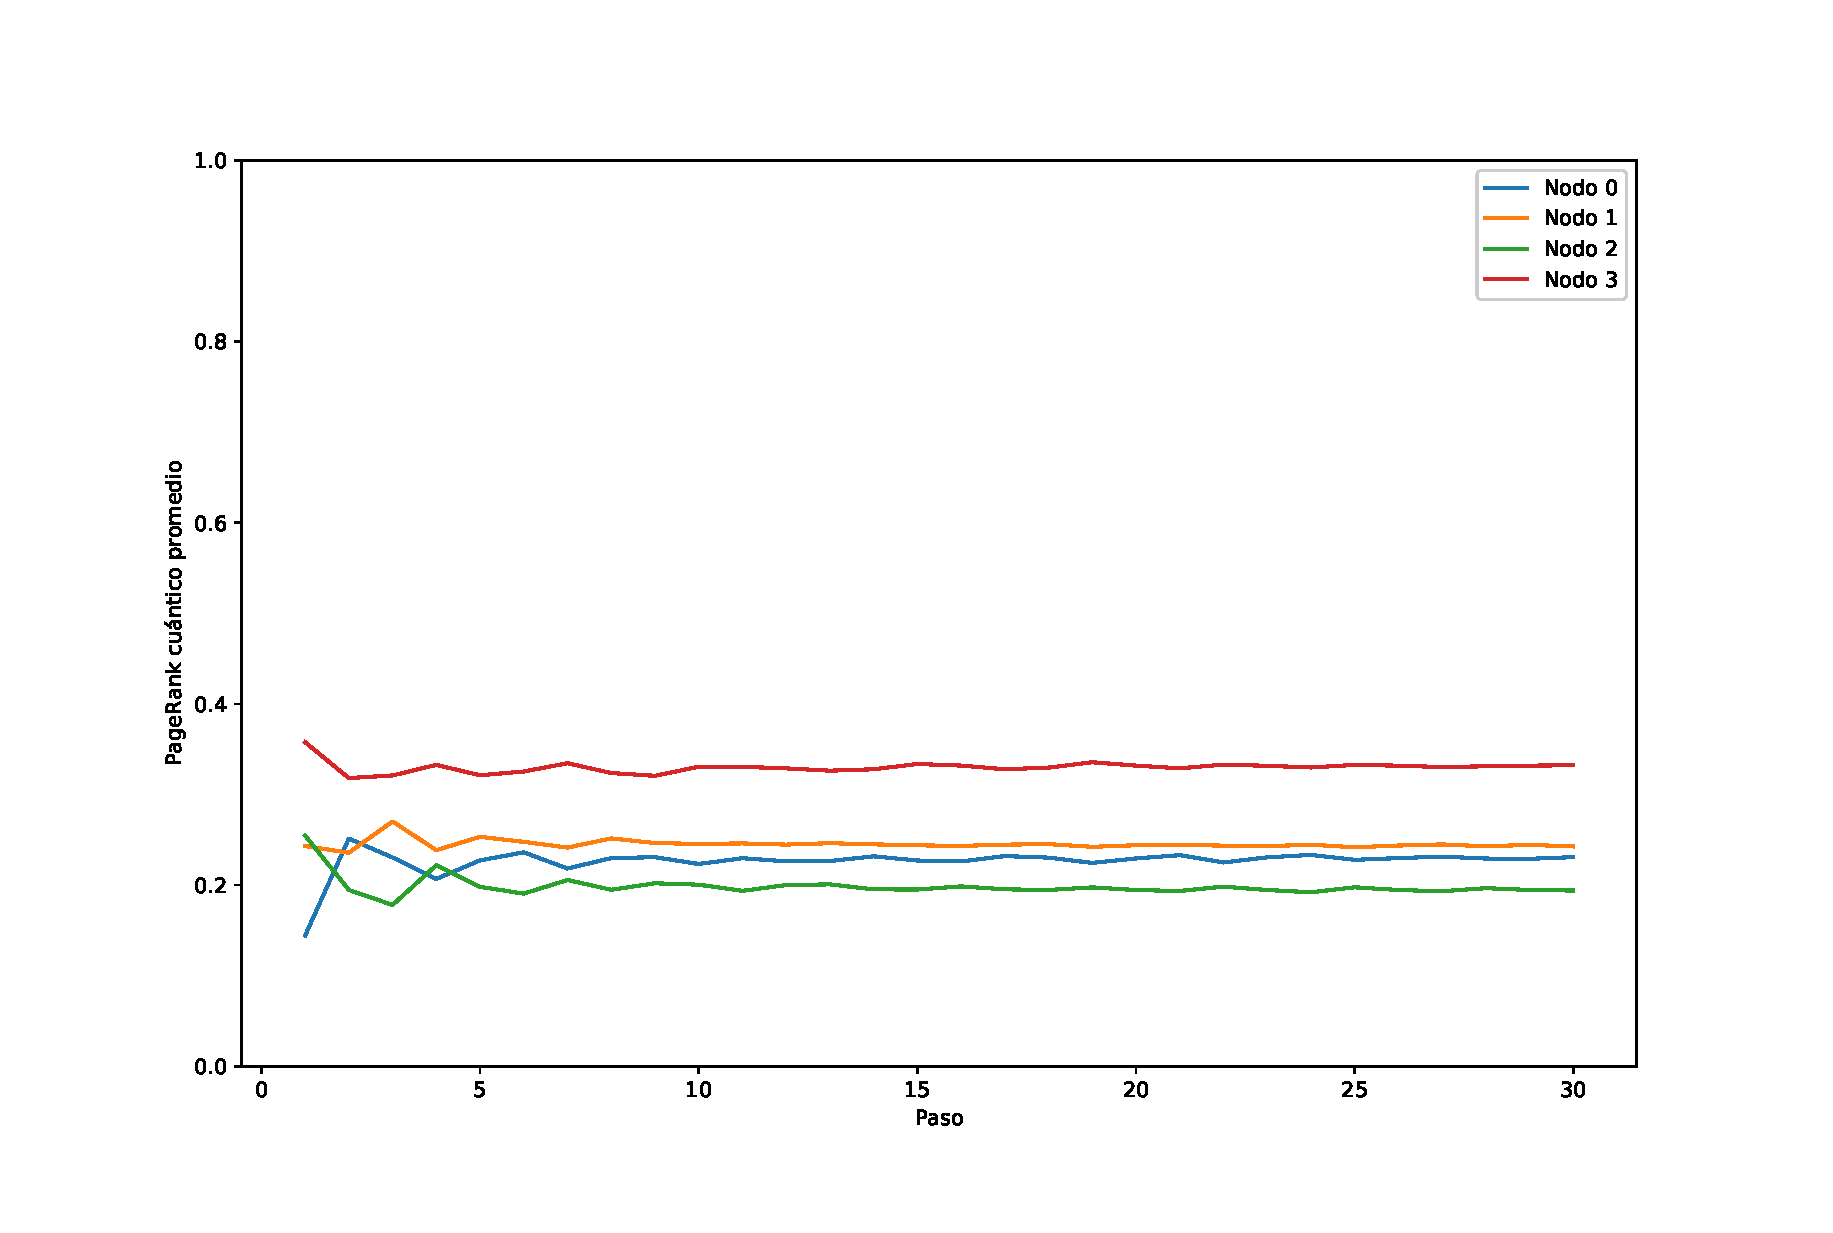
\includegraphics[width=0.9\linewidth]{img/tree-mean-lossless.eps}
        \caption{Sin relajación}
    \end{subfigure}
    \begin{subfigure}[m]{0.45\textwidth}
        \centering
        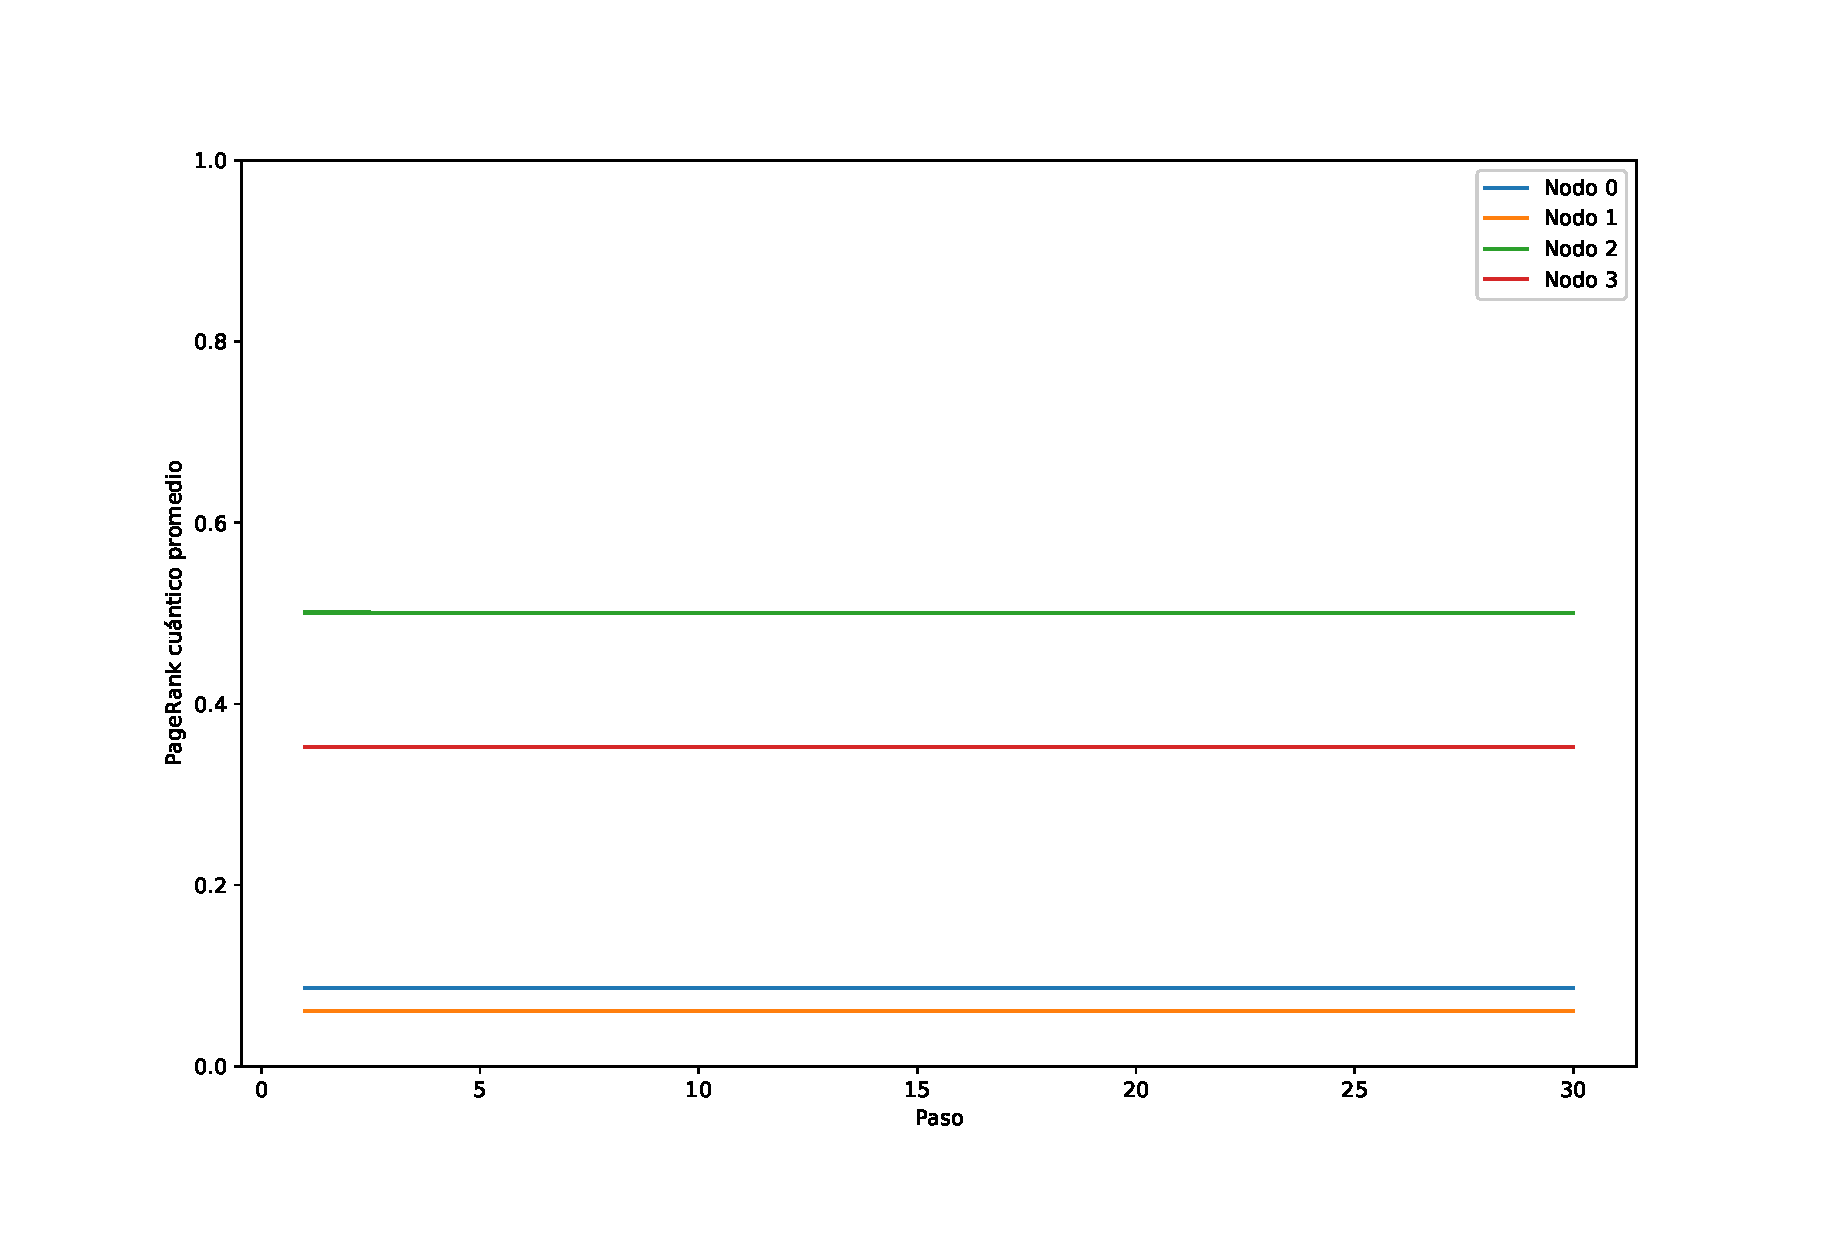
\includegraphics[width=0.9\linewidth]{img/tree-mean-lossy.eps}
        \caption{Con relajación}
    \end{subfigure}
    \caption[PageRank cuántico promedio del grafo árbol con y sin pérdidas]{PageRank cuántico promedio del grafo árbol con y sin pérdidas}
    \label{fig:meantreelossy}
\end{figure}














\begin{figure}[H]
    \centering
    \begin{tikzpicture}[->,>=stealth',shorten >=1pt,thick]
    \SetGraphUnit{2} 
    \tikzset{VertexStyle/.style = {draw,circle,thick,
                                   minimum size=0.5cm,
                                   font=\bfseries},thick} 
    \Vertex{1} \SOWE(1){2} \SOEA(1){3} \SOEA(2){4} 
    \Edge(1)(2)
    \Edge(1)(3)
    \Edge(1)(4)
    \Edge(2)(4)
    \Edge(3)(4)

    \tikzset{EdgeStyle/.style = {->, bend left}}
    \Edge(2)(1)
    \tikzset{EdgeStyle/.style = {->, bend right}}
    \Edge(4)(3)
    \end{tikzpicture} 
    \caption[Grafo aleatorio]{Grafo aleatorio}
    \label{fig:any}
\end{figure}

\begin{equation}
    A =
    \begin{pmatrix}
        0 & 1 & 0 & 0 \\
        1 & 0 & 0 & 0 \\
        1 & 0 & 0 & 1 \\
        1 & 1 & 1 & 0 \\
    \end{pmatrix}
\end{equation}

\begin{equation}
    E =
    \begin{pmatrix}
        0 & \frac{1}{2} & 0 & 0 \\
        \frac{1}{3} & 0 & 0 & 0 \\
        \frac{1}{3} & 0 & 0 & 1 \\
        \frac{1}{3} & \frac{1}{2} & 1 & 0 \\
    \end{pmatrix}
\end{equation}

\begin{equation}
    G =
    \begin{pmatrix}
        \frac{3}{80} & \frac{37}{80} & \frac{3}{80} & \frac{3}{80} \\
        \frac{77}{240} & \frac{3}{80} & \frac{3}{80} & \frac{3}{80} \\
        \frac{77}{240} & \frac{3}{80} & \frac{3}{80} & \frac{71}{80} \\
        \frac{77}{240} & \frac{37}{80} & \frac{71}{80} & \frac{3}{80} \\
    \end{pmatrix}
\end{equation}

\begin{figure}[H]
\[\Qcircuit @C=1.4em @R=1.8em {
& \gate{Ry(1.85806)} & \ctrlo{1}           & \ctrl{1}          & \qw \\
& \qw                & \gate{Ry(2.48274)}  & \gate{Ry(1.5708)} & \qw \\
} \]
\caption{Circuito de $K_1$ para el grafo aleatorio}
\label{fig:anykb1}
\end{figure}

\begin{figure}[H]
\[\Qcircuit @C=1.4em @R=1.8em {
& \gate{Ry(1.5708)} & \ctrlo{1}           & \ctrl{1}          & \qw \\
& \qw                & \gate{Ry(0.554811)}  & \gate{Ry(2.58678)} & \qw \\
} \]
\caption{Circuito de $K_2$ para el grafo aleatorio}
\label{fig:anykb2}
\end{figure}

\begin{figure}[H]
\[\Qcircuit @C=1.4em @R=1.8em {
& \gate{Ry(2.58678)} & \ctrlo{1}           & \ctrl{1}          & \qw \\
& \qw                & \gate{Ry(1.5708)}  & \gate{Ry(2.73613)} & \qw \\
} \]
\caption{Circuito de $K_3$ para el grafo aleatorio}
\label{fig:anykb3}
\end{figure}

\begin{figure}[H]
\[\Qcircuit @C=1.4em @R=1.8em {
& \ctrlo{1}          & \ctrlo{1}          & \ctrl{2}           & \qw \\
& \ctrlo{1}          & \ctrl{1}           & \qw                & \qw \\
& \multigate{1}{K_1} & \multigate{1}{K_2} & \multigate{1}{K_3} & \qw \\
& \ghost{K_1}        & \ghost{K_2}        & \ghost{K_3}        & \qw \\
} 
\]
\caption[$K_b$ del grafo aleatorio]{$K_b$ del grafo aleatorio}
\label{fig:anykb}
\end{figure}

\begin{figure}[H]
\[\Qcircuit @C=1.4em @R=1.8em {
& \ctrl{1}  & \ctrl{1} & \qw \\
& \ctrl{1}  & \ctrl{2} & \qw \\
& \targ     & \qw      & \qw \\
& \ctrl{-1} & \targ    & \qw \\
} 
\]
\caption[$T$ del grafo aleatorio]{$T$ del grafo aleatorio}
\label{fig:anyT}
\end{figure}

\begin{figure}[H]
\[\Qcircuit @C=1.4em @R=1.8em {
& \gate{H} & \multigate{3}{K_b} & \multigate{3}{T^\dagger} & \qw \\
& \gate{H} & \ghost{K_b}        & \ghost{T^\dagger}        & \qw \\
& \qw      & \ghost{K_b}        & \ghost{T^\dagger}        & \qw \\
& \qw      & \ghost{K_b}        & \ghost{T^\dagger}        & \qw \\
} 
\]
\caption{Preparación del estado inicial para la caminata en el grafo aleatorio}
\label{fig:anyinit}
\end{figure}

\begin{figure}[H]
\[ \Qcircuit @C=1.4em @R=1.8em {
\lstick{\ket{0}} & {/^4} \qw & \gate{Init} & \gate{T} & \gate{K_b^\dagger} & \gate{D} & \gate{K_b} & \gate{T^\dagger} & \gate{SWAP} & \meter & \cw \\
& & & & \rstick{ 2m \text{ veces}}
\gategroup{1}{4}{1}{9}{1.3em}{_\}}
} \]
\caption{Circuito del PageRank cuántico  del grafo aleatorio}
\label{fig:lokeany}
\end{figure}

\begin{figure}[H]
    \centering
    \begin{subfigure}[m]{0.45\textwidth}
        \centering
        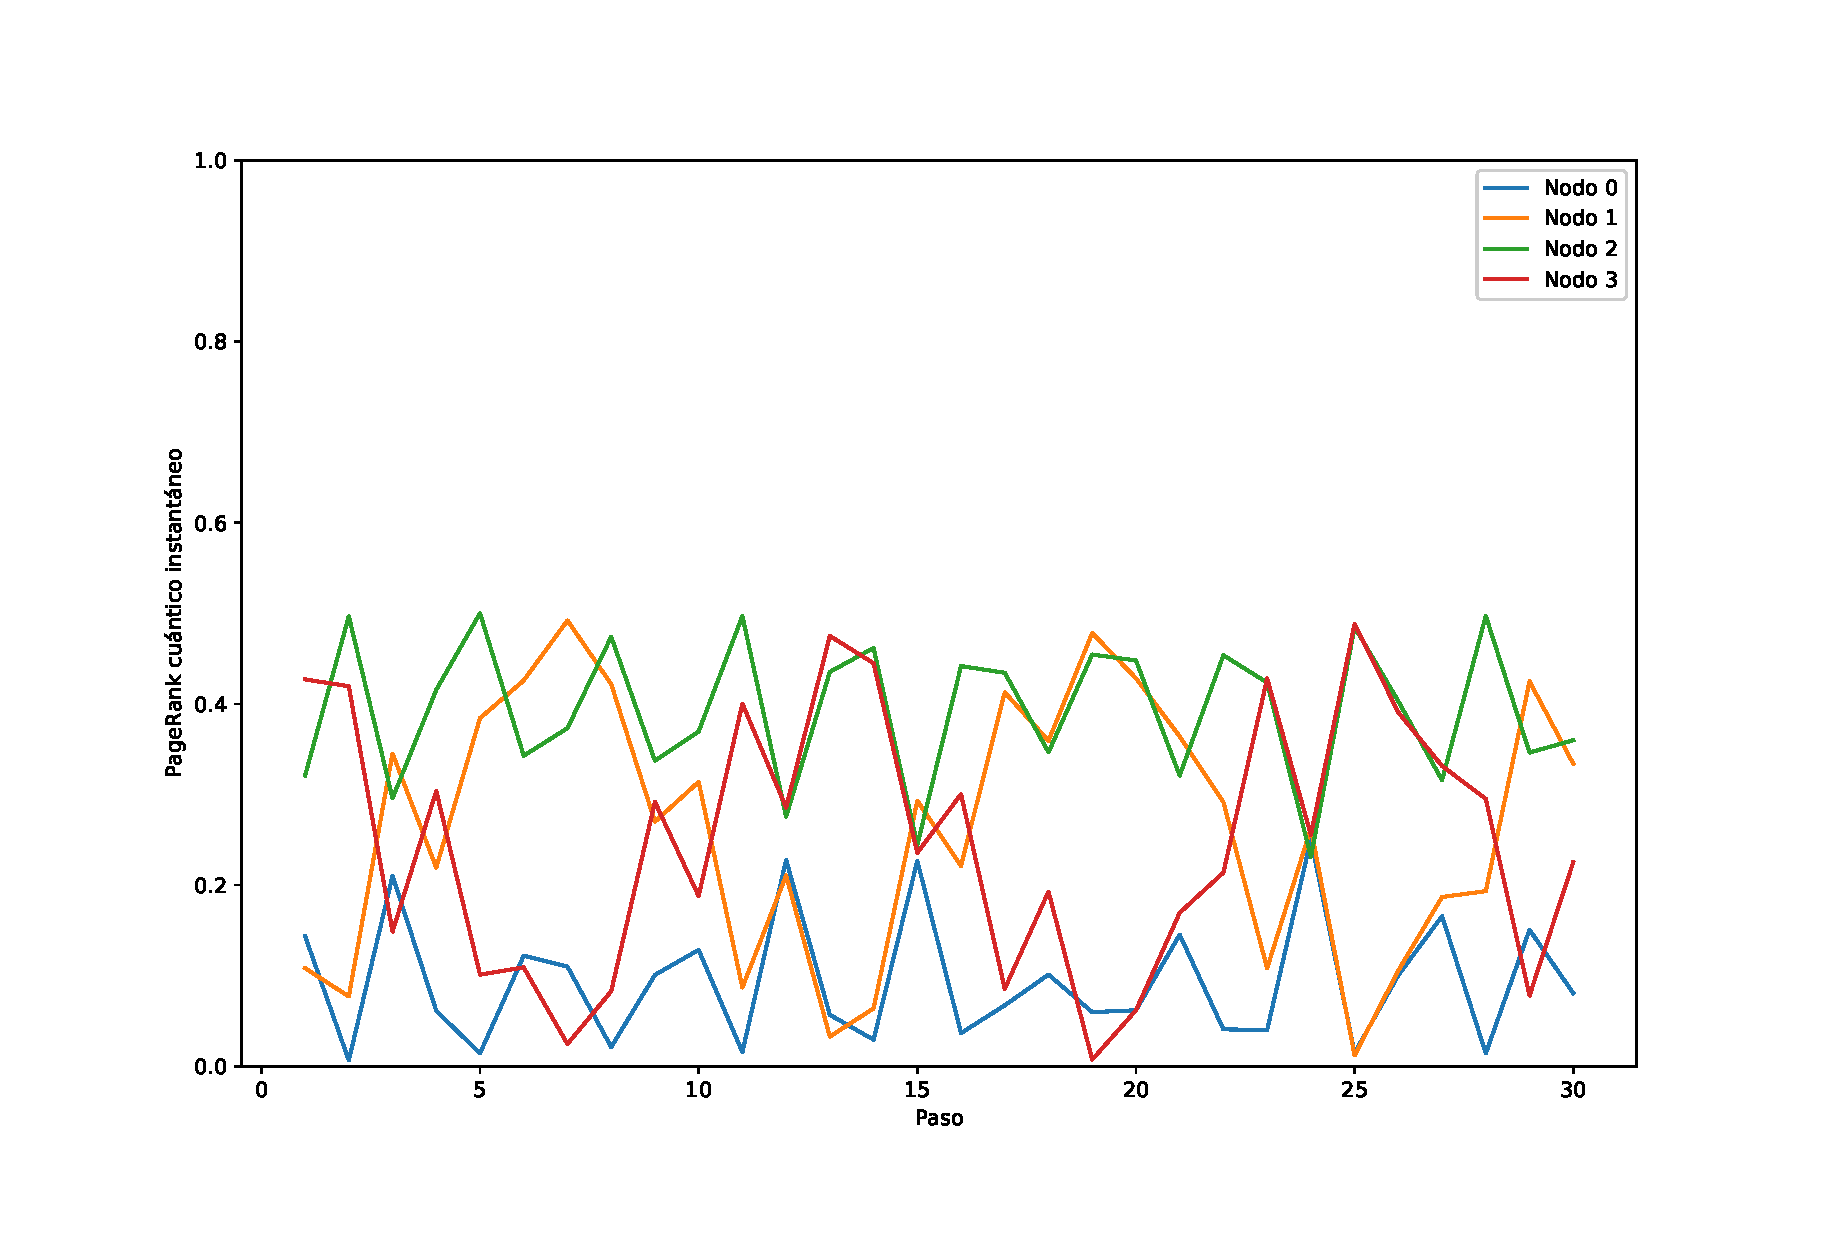
\includegraphics[width=0.9\linewidth]{img/any-inst-M.eps}
        \caption{Wolfram Mathematica}
    \end{subfigure}
    \begin{subfigure}[m]{0.45\textwidth}
        \centering
        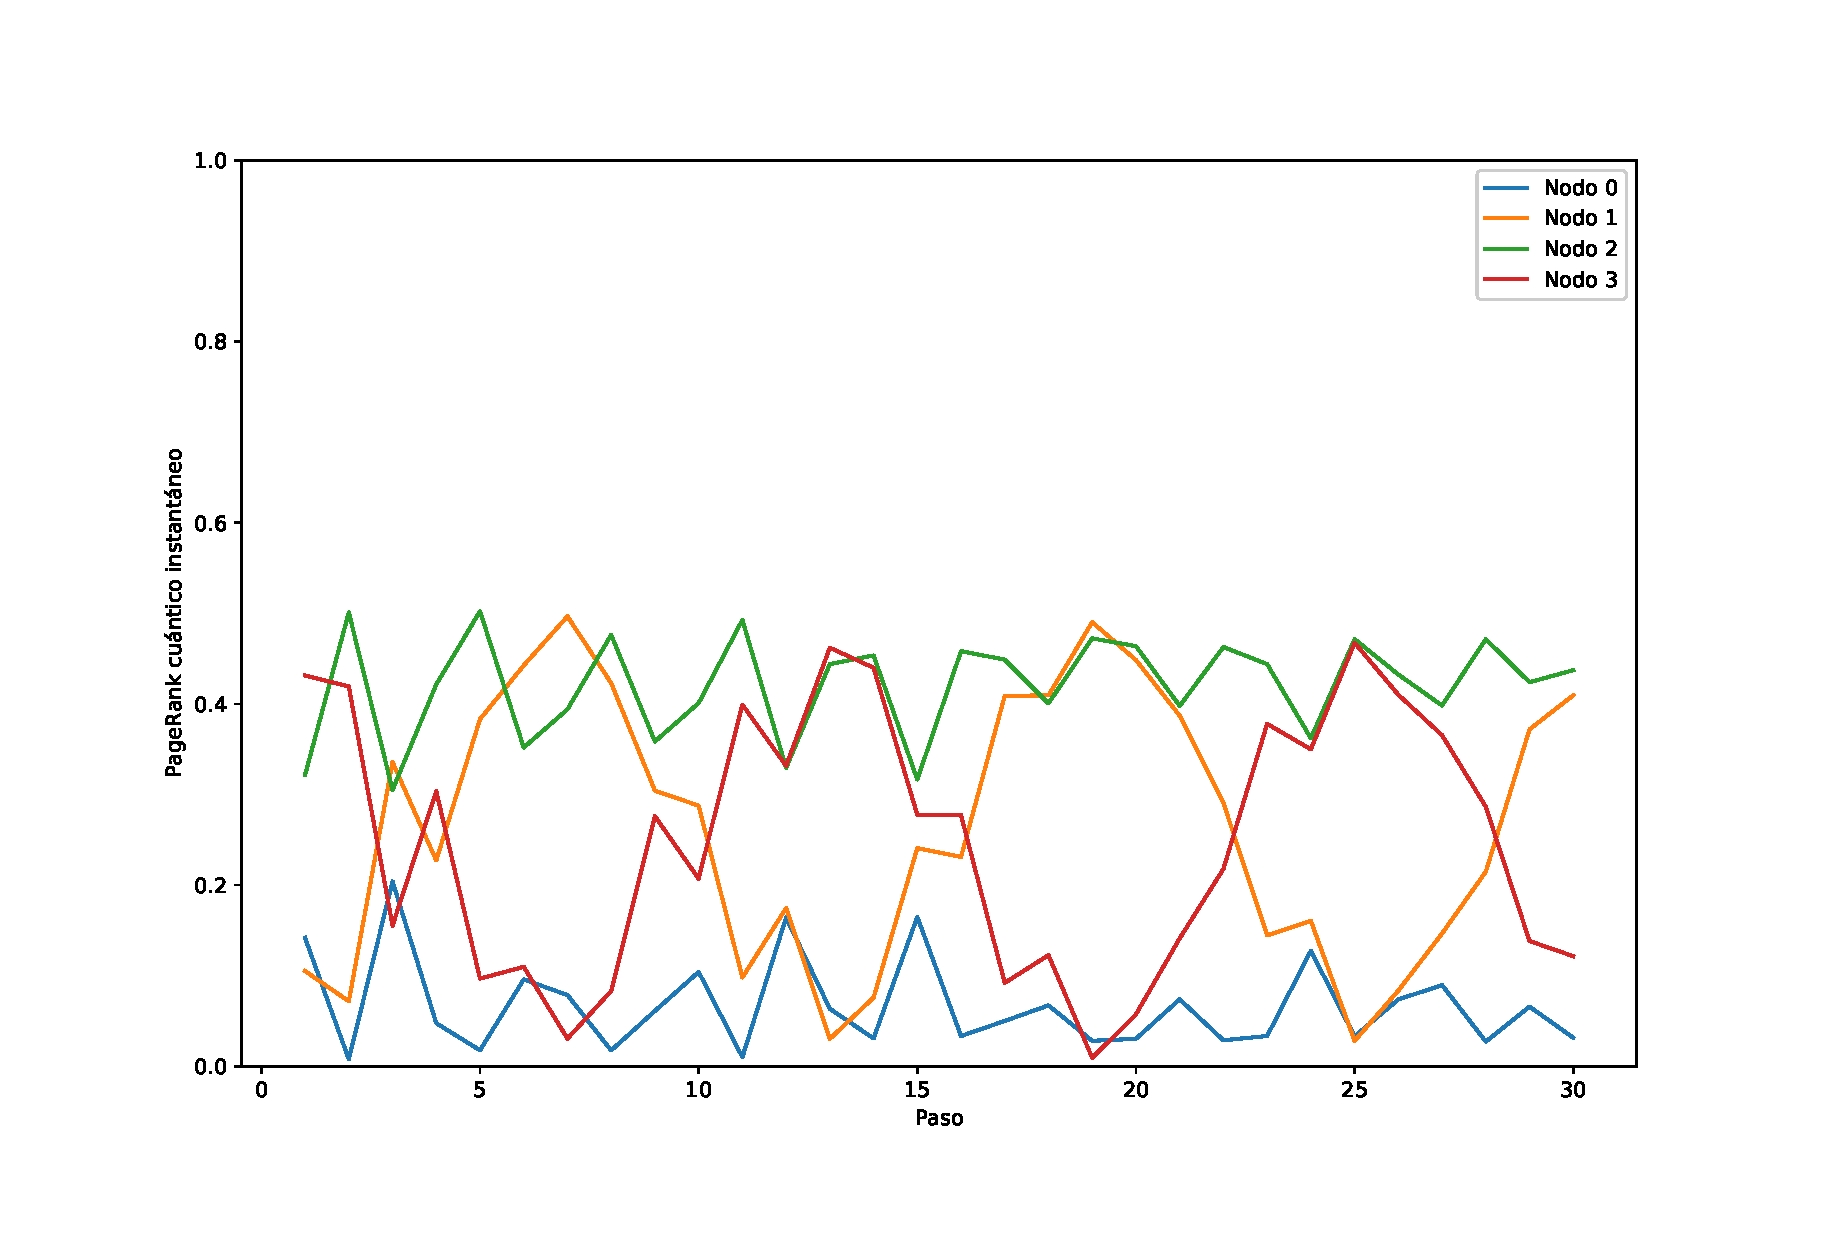
\includegraphics[width=0.9\linewidth]{img/any-inst-lossless.eps}
        \caption{Python}
    \end{subfigure}
    \caption[PageRank cuántico instantáneo del grafo aleatorio sin pérdidas]{PageRank cuántico instantáneo del grafo aleatorio sin pérdidas}
    \label{fig:instanylossless}
\end{figure}

\begin{figure}[H]
    \centering
    \begin{subfigure}[m]{0.45\textwidth}
        \centering
        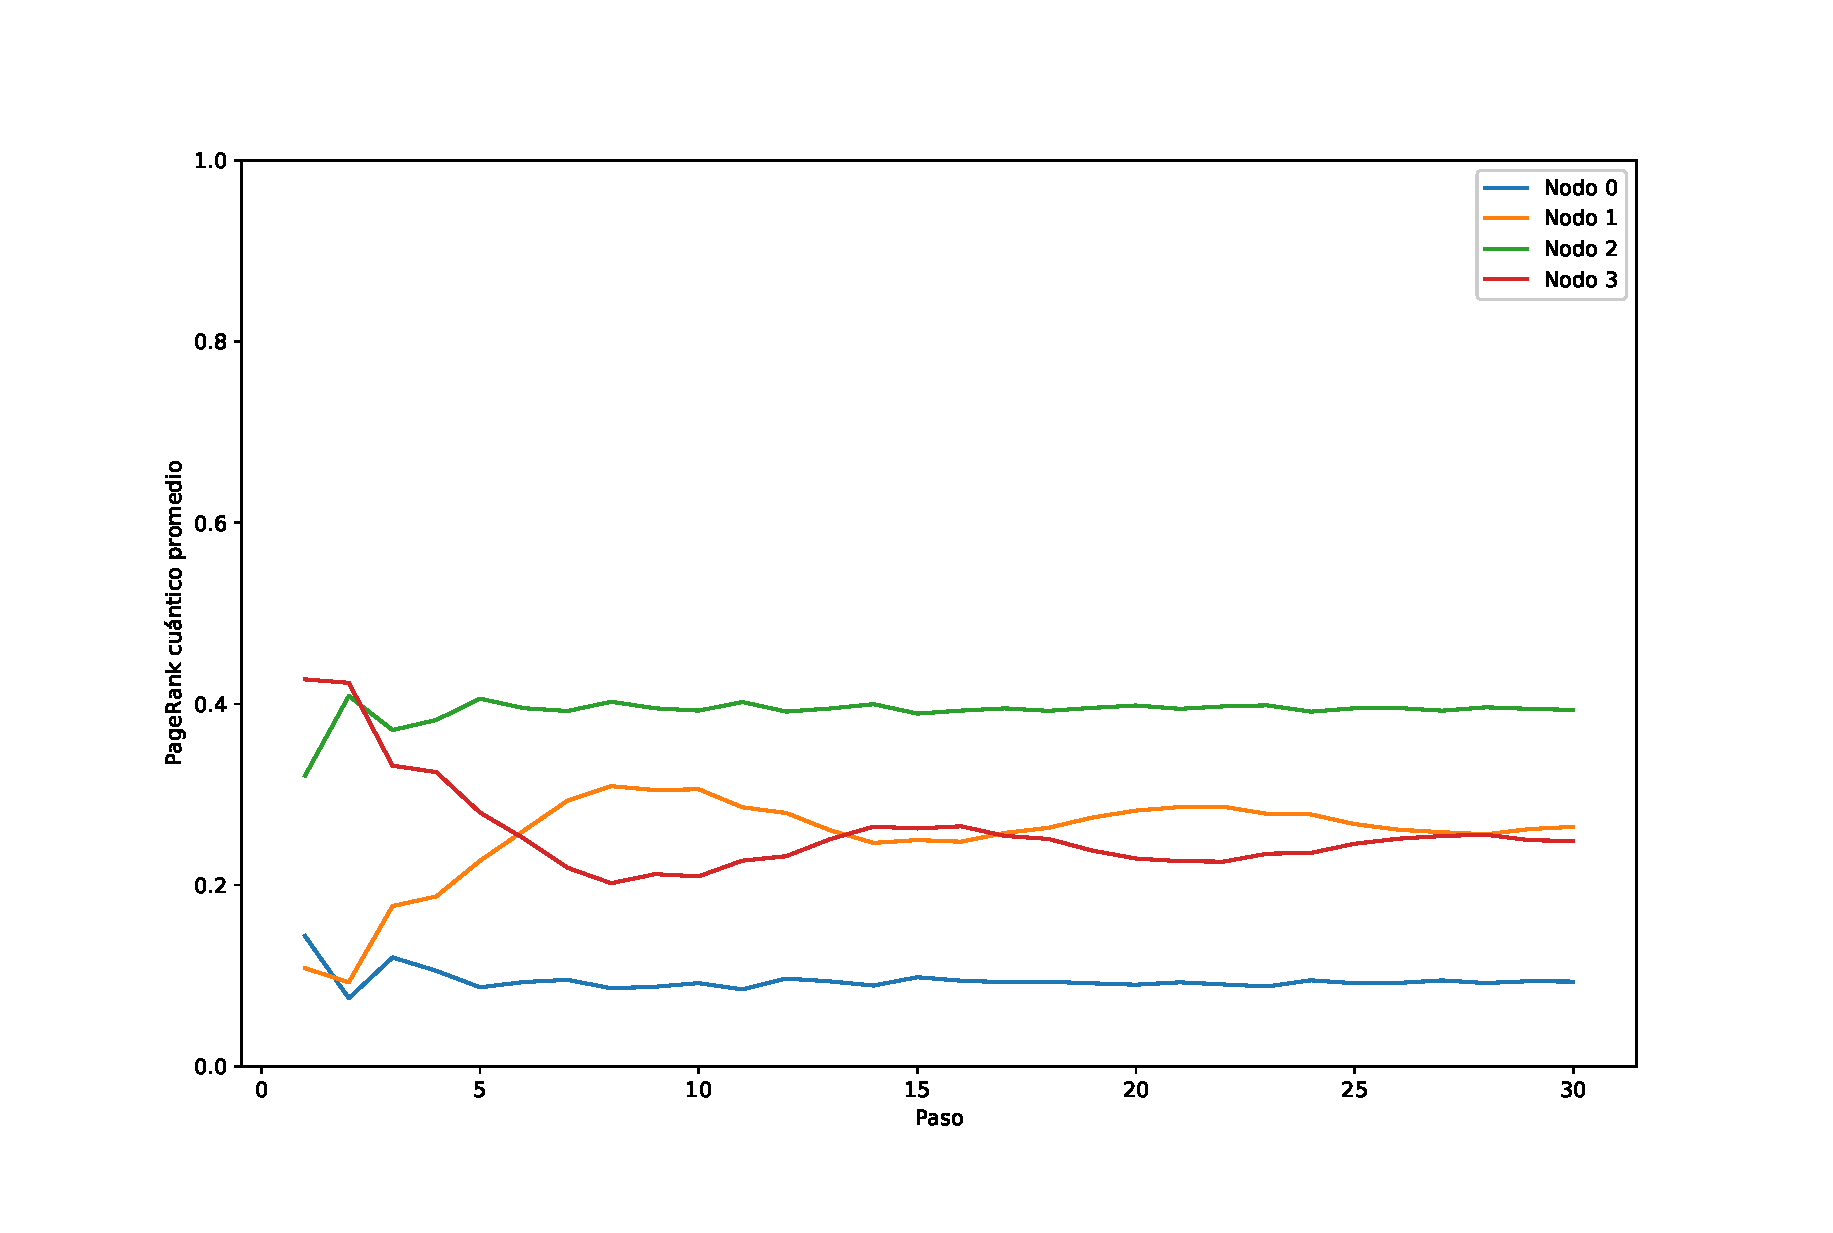
\includegraphics[width=0.9\linewidth]{img/any-mean-M.eps}
        \caption{Wolfram Mathematica}
    \end{subfigure}
    \begin{subfigure}[m]{0.45\textwidth}
        \centering
        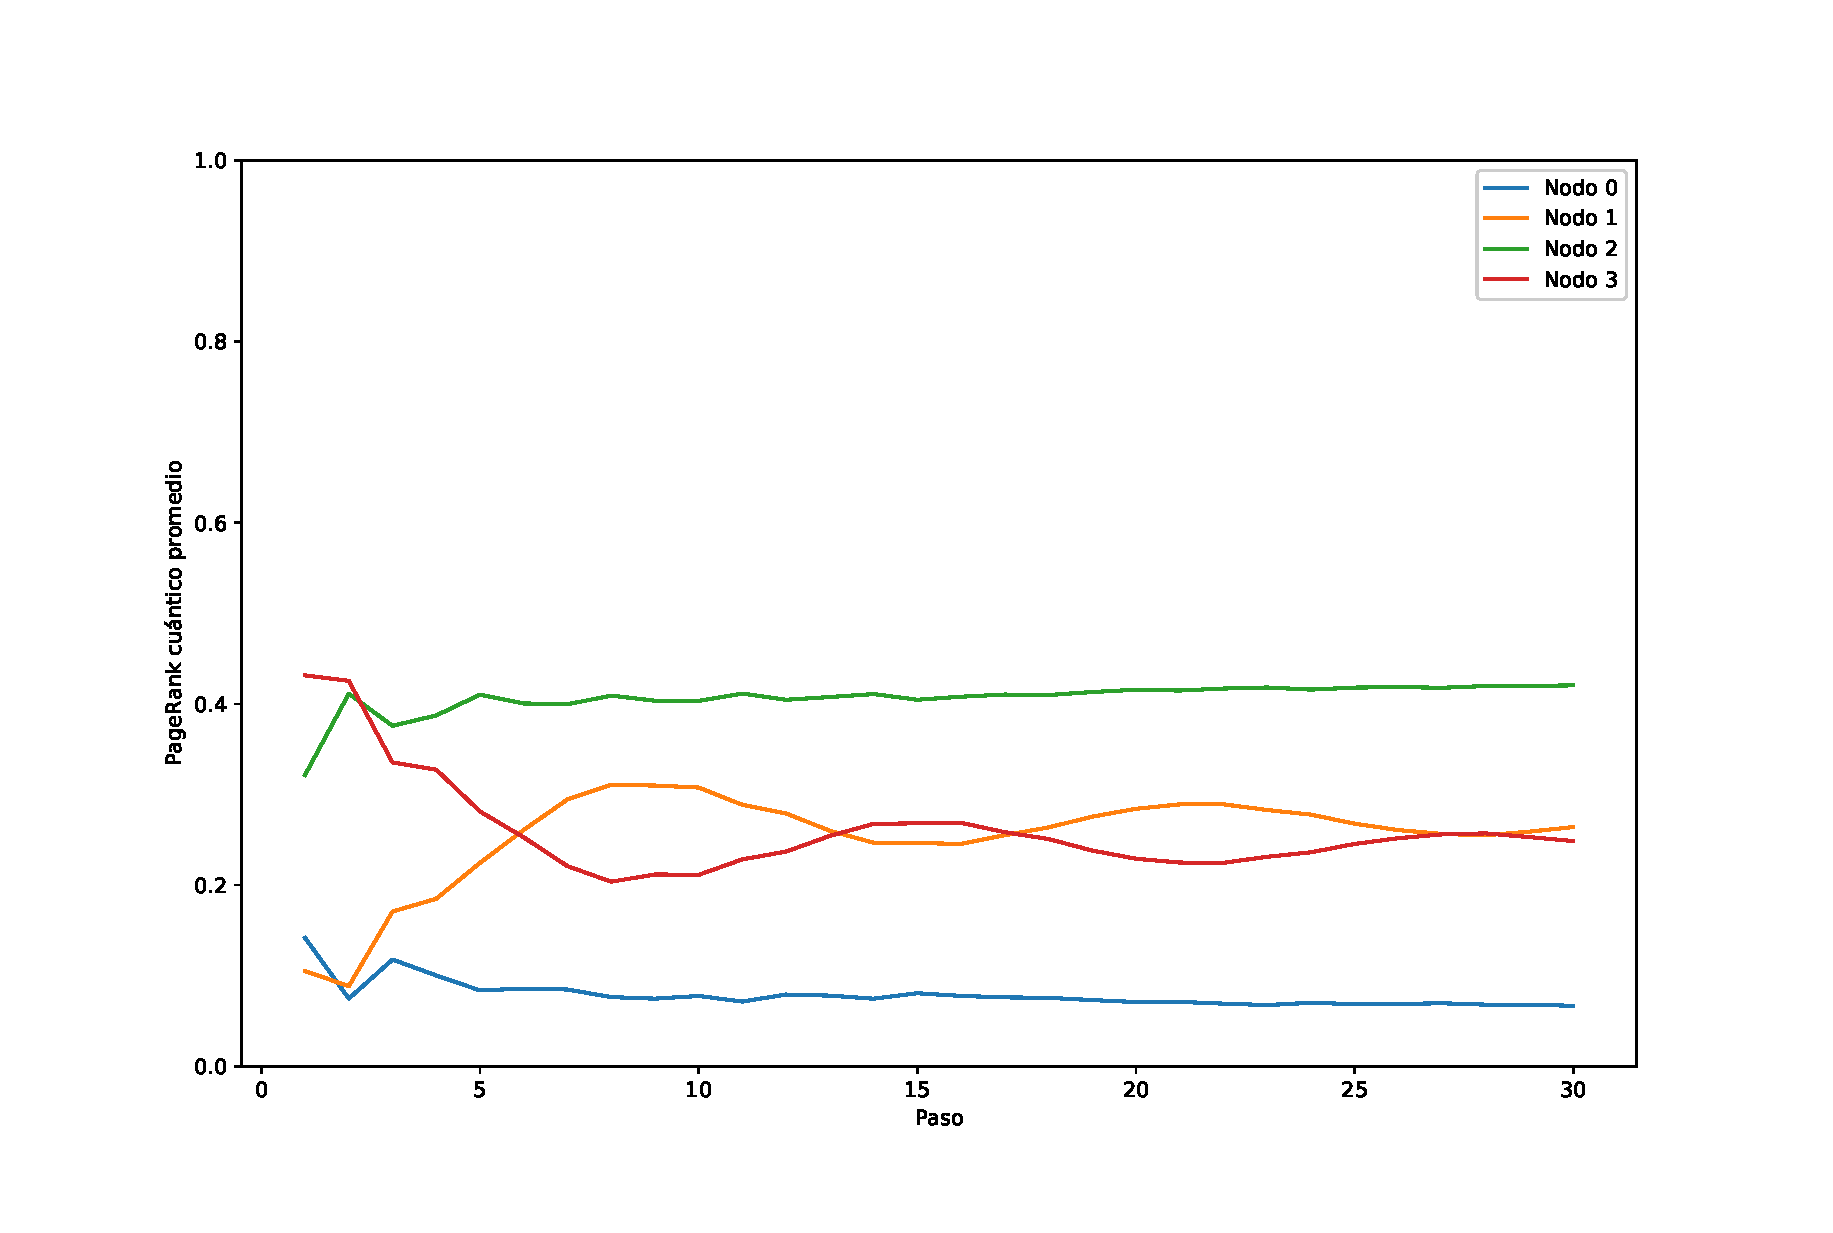
\includegraphics[width=0.9\linewidth]{img/any-mean-lossless.eps}
        \caption{Python}
    \end{subfigure}
    \caption[PageRank cuántico promedio del grafo aleatorio sin pérdidas]{PageRank cuántico promedio del grafo aleatorio sin pérdidas}
    \label{fig:meananylossless}
\end{figure}

\begin{figure}[H]
    \centering
    \begin{subfigure}[m]{0.45\textwidth}
        \centering
        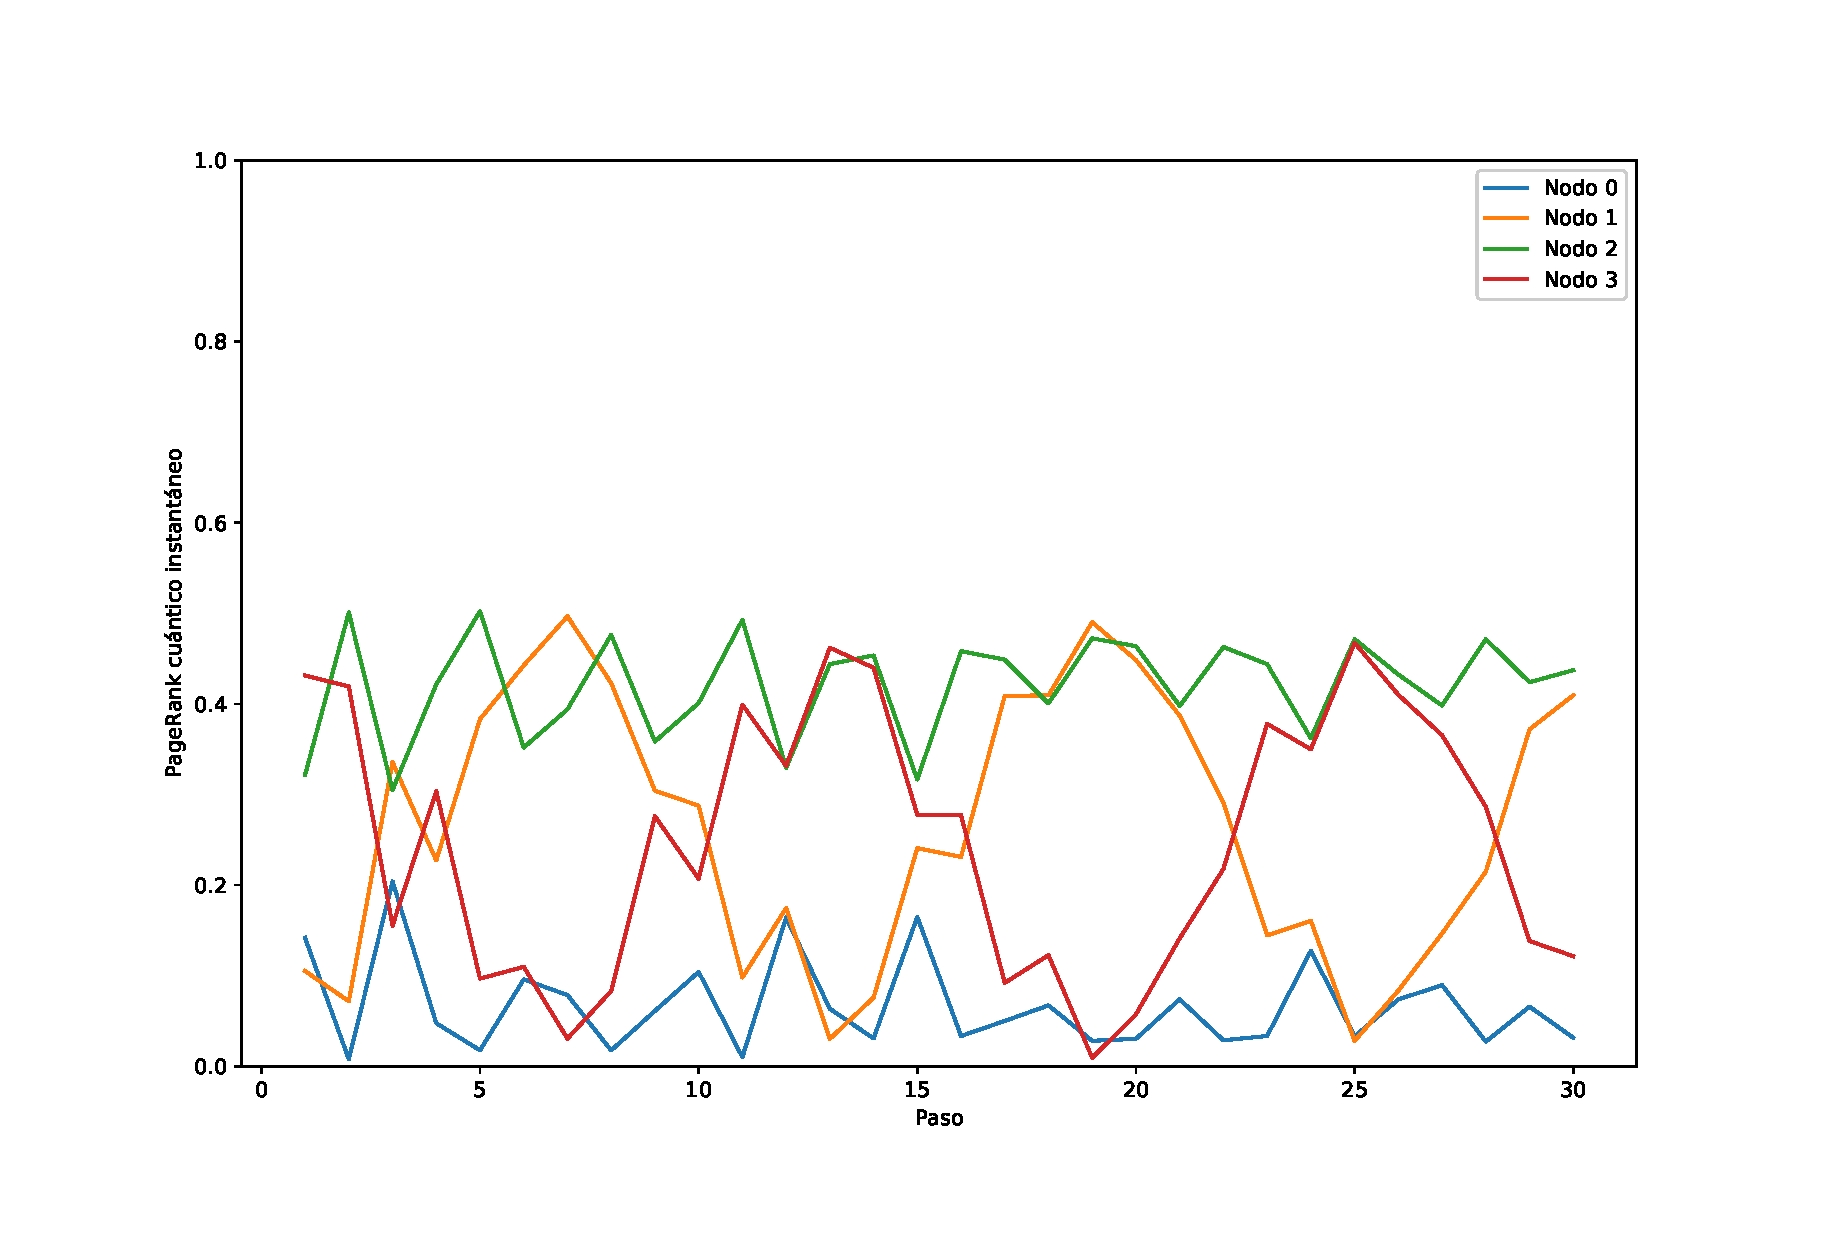
\includegraphics[width=0.9\linewidth]{img/any-inst-lossless.eps}
        \caption{Sin relajación}
    \end{subfigure}
    \begin{subfigure}[m]{0.45\textwidth}
        \centering
        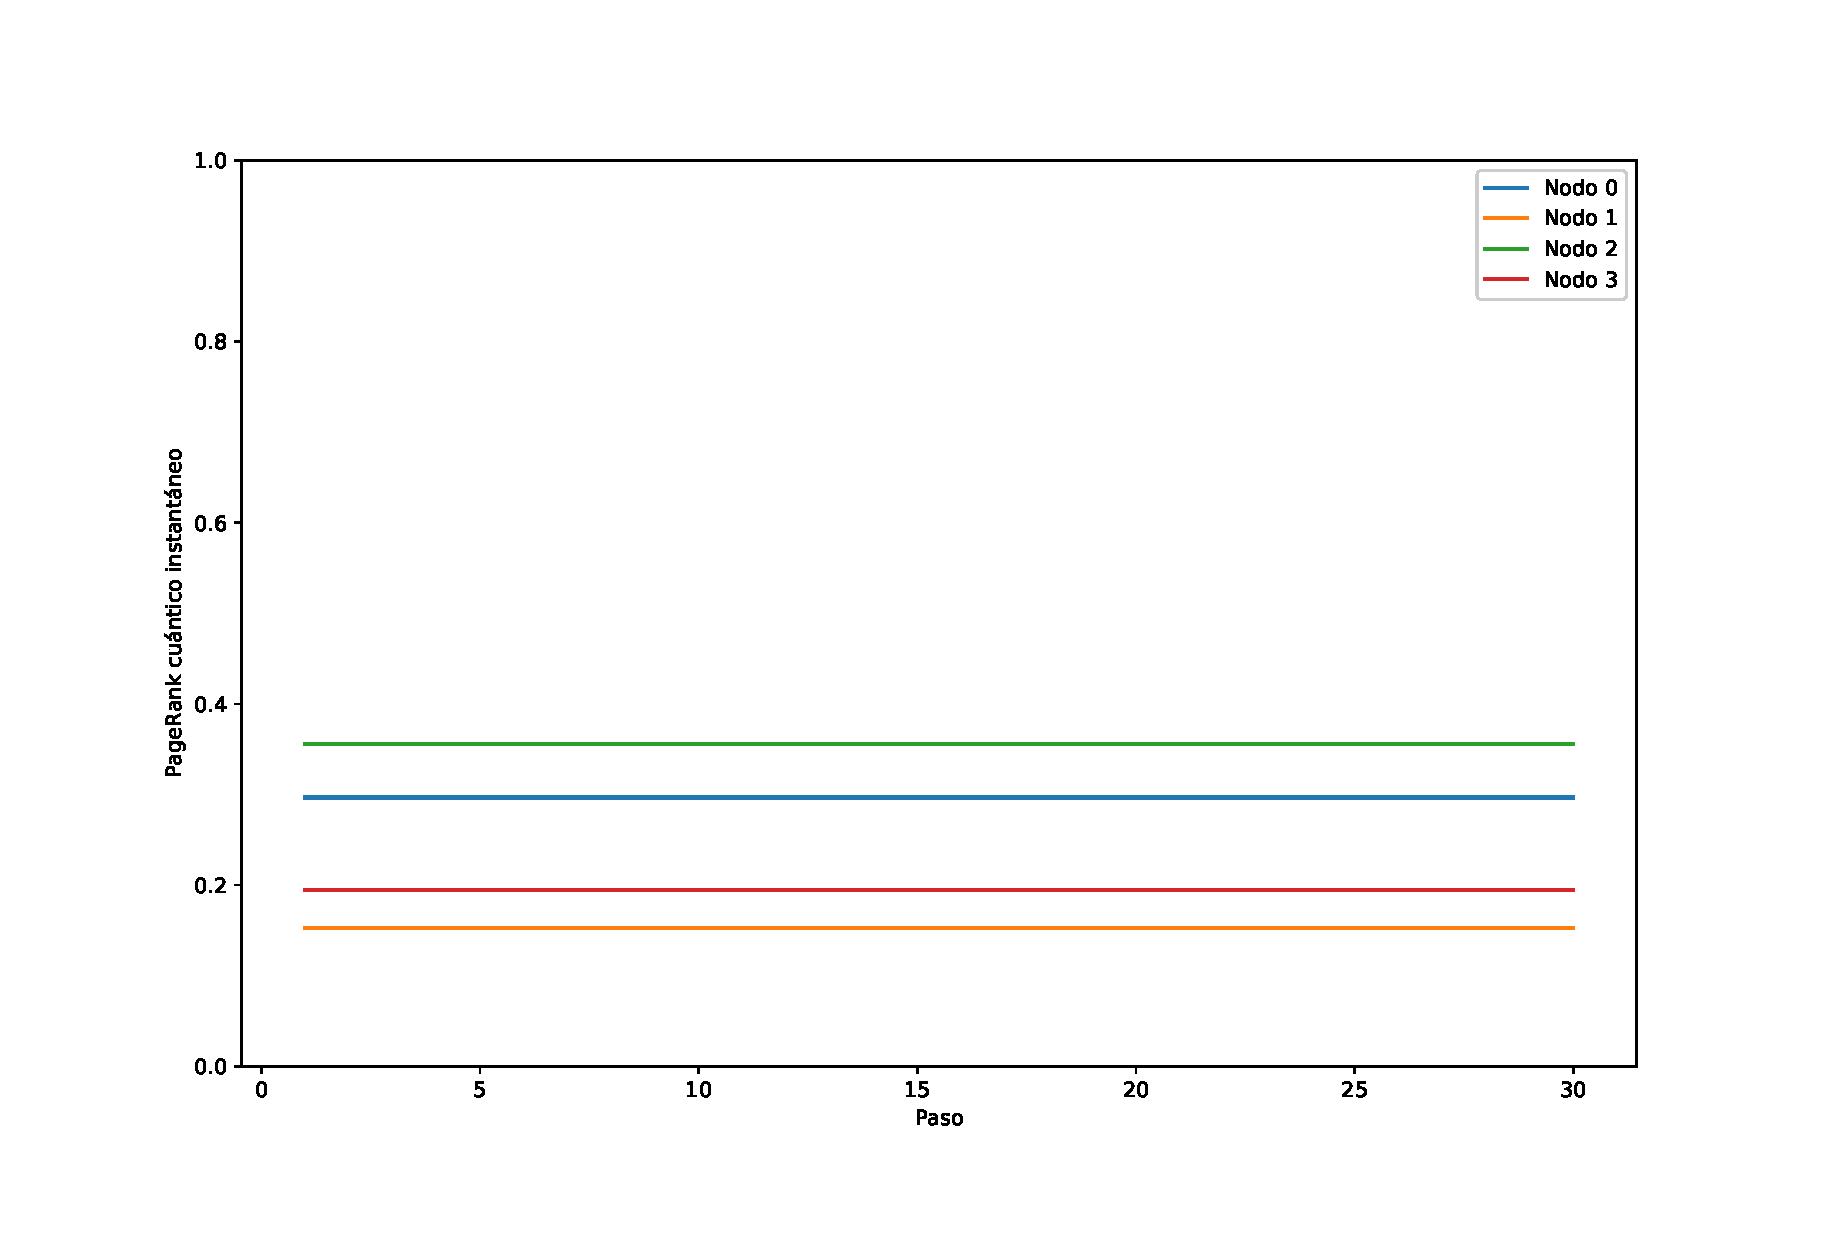
\includegraphics[width=0.9\linewidth]{img/any-inst-lossy.eps}
        \caption{Con relajación}
    \end{subfigure}
    \caption[PageRank cuántico instantaneo del grafo aleatorio con y sin pérdidas]{PageRank cuántico instantaneo del grafo aleatorio con y sin pérdidas}
    \label{fig:instanylossy}
\end{figure}

\begin{figure}[H]
    \centering
    \begin{subfigure}[m]{0.45\textwidth}
        \centering
        \includegraphics[width=0.9\linewidth]{img/any-mean-lossless.eps}
        \caption{Sin relajación}
    \end{subfigure}
    \begin{subfigure}[m]{0.45\textwidth}
        \centering
        \includegraphics[width=0.9\linewidth]{img/any-mean-lossy.eps}
        \caption{Con relajación}
    \end{subfigure}
    \caption[PageRank cuántico promedio del grafo aleatorio con y sin pérdidas]{PageRank cuántico promedio del grafo aleatorio con y sin pérdidas}
    \label{fig:meananylossy}
\end{figure}


\end{frame}

\section{Conclusiones}

\begin{frame}
    \frametitle{Conclusiones}

En el presente trabajo, se desarrollaron las siguientes herramientas y se obtuvieron los siguientes resultados novedosos:

\begin{enumerate}
    \item Una compuerta controlada de fase CP que permita eliminar las fases en las compuertas de negación con dos o más qubits de control, como la de Toffoli.
    \item Un conjunto de instrucciones cuánticas basadas en las compuertas nativas de los transmones y un simulador del sistema físico.
    \item Un operador de multiplicación por 3 módulo 8 sin qubits de ancilla.
    \item La forma explícita del operador de difusión de las caminatas cuánticas de Szegedy para grafos de cuatro nodos, en función de rotaciones en Y controladas.
    \item El efecto de la relajación en los algoritmos de Grover, Shor y PageRank.
\end{enumerate}

Los resultados de las simulaciones del algoritmo de Grover y PageRank nos indican que para sistemas con tiempos de relajación del orden de $O(10^4 ns)$, los protocolos de corrección de errores son una necesidad. Este es un resultado significante, pues el record actual de tiempo de vida de un qubit superconductor es inferior a 0.1ms, está en el mismo orden de magnitud que el del sistema simulado.

\end{frame}


\end{document}

